\documentclass[12pt, a4paper]{report}

% ==========================================
% PACKAGES
% ==========================================
\usepackage[utf8]{inputenc}
\usepackage[T1]{fontenc}
\usepackage{geometry}
\geometry{left=1.5in, right=1in, top=1in, bottom=1in}
\usepackage{setspace}
\doublespacing
\usepackage{graphicx}
\usepackage{float}
\usepackage{amsmath}
\usepackage{amssymb}
\usepackage{booktabs}
\usepackage{longtable}
\usepackage{array}
\usepackage{cite}
\usepackage{hyperref}
\usepackage{titlesec}
\usepackage{tocloft}
\usepackage{fancyhdr}
\usepackage{enumitem}
\usepackage{multirow}
\usepackage{makecell}

% ==========================================
% PAGE AND HEADER FORMATTING
% ==========================================
\pagestyle{fancy}
\fancyhf{}
\fancyhead[R]{\thepage}
\renewcommand{\headrulewidth}{0pt}

% ==========================================
% CHAPTER & SECTION FORMATTING (FIXED)
% ==========================================
\titleformat{\chapter}[display]
  {\normalfont\bfseries\centering}
  {\chaptertitlename\ \thechapter}
  {10pt}
  {\MakeUppercase}
\titlespacing*{\chapter}{0pt}{-20pt}{20pt}

\titleformat{\section}
  {\normalfont\bfseries}
  {\thesection}{1em}{}

\titleformat{\subsection}
  {\normalfont\bfseries}
  {\thesubsection}{1em}{}

% ==========================================
% DOCUMENT START
% ==========================================
\begin{document}

% --- I-set ang section numbering to 1.1, 1.2, etc. ---
\renewcommand{\thesection}{\thechapter.\arabic{section}}

% ==========================================
% PRELIMINARY PAGES
% ==========================================
\pagenumbering{roman}

% --- TITLE PAGE ---
\begin{titlepage}
    \begin{singlespace}
    \centering
    {\Large\bfseries GIS-INTEGRATED CHILD NUTRITION MONITORING SYSTEM WITH AI-BASED DECISION SUPPORT AND AUTOMATED ALERTS FOR CHILD MALNUTRITION MANAGEMENT IN CABADBARAN CITY \par}
    \vspace{1cm}
    {\normalsize A CAPSTONE PROJECT SUBMITTED TO THE FACULTY OF THE COLLEGE OF ENGINEERING AND INFORMATION TECHNOLOGY, CARAGA STATE UNIVERSITY CABADBARAN CAMPUS, CABADBARAN CITY, AGUSAN DEL NORTE \par}
    \vspace{0.5cm}
    {\normalsize IN PARTIAL FULFILLMENT OF THE REQUIREMENTS FOR THE DEGREE OF BACHELOR OF SCIENCE IN INFORMATION TECHNOLOGY \par}
    \vspace{3cm}
    {\normalsize BY: \par}
    \vspace{0.1cm}
    {\normalsize BALDOMAR, KENNETH A. \par}
    \vspace{0.1cm}
    {\normalsize LORENZO, EUNICE G. \par}
    \vspace{0.1cm}
    {\normalsize PALCO, NATHANIEL G. \par}
    \vspace{2.5cm}
    {\normalsize ADVISER: \par}
    \vspace{0.1cm}
    {\normalsize MR. MARIO B. CADAY, MSIT \par}
    \vspace{2cm}
    {\normalsize NOVEMBER 2026 \par}
    \end{singlespace}
\end{titlepage}

% --- APPROVAL SHEET ---
\clearpage
\thispagestyle{plain}
\begin{singlespace}
\begin{center}
    \Large \textbf{APPROVAL SHEET}
\end{center}
\vspace{0.2cm}

The Capstone manuscript attached hereto, entitled \textbf{``GIS-INTEGRATED CHILD NUTRITION MONITORING SYSTEM WITH AI-BASED DECISION SUPPORT AND AUTOMATED ALERTS FOR CHILD MALNUTRITION MANAGEMENT IN CABADBARAN CITY''} prepared and submitted by Baldomar, Kenneth A., Lorenzo, Eunice G., and Palco, Nathaniel G., in partial fulfillment of the requirements for the degree of Bachelor of Science in Information Technology, is hereby recommended for approval.

\vspace{0.4cm}

\begin{center}
    \rule{7cm}{0.5pt} \\
    \vspace{0.1cm} 
    \textbf{MARIO B. CADAY, MSIT} \\
    \vspace{0.2cm} 
    Adviser \\
    \vspace{0.1cm} 
    Date Signed
\end{center}

\vspace{0.2cm}
\noindent
\begin{flushleft}
    Examination Panel:
\end{flushleft}
\vspace{0.4cm}

\begin{center}
    \rule{7cm}{0.5pt} \\
    \vspace{0.1cm}
    \textbf{Lead Panel} \\
    \vspace{0.2cm}
    Date Signed
\end{center}

\vspace{0.4cm}
\noindent
\begin{center}
    \begin{tabular}{c c}
        \rule{6.5cm}{0.5pt} & \rule{6.5cm}{0.5pt} \\
        \vspace{0.1cm} & \vspace{0.1cm} \\
        \textbf{Panel} & \textbf{Panel} \\
        \vspace{0.2cm} & \vspace{0.2cm} \\
        Date Signed & Date Signed
    \end{tabular}
\end{center}

\vspace{0.4cm}

This capstone project is approved in partial fulfillment of the requirements for the degree of Bachelor of Science in Information Technology.

\vspace{0.6cm}

\begin{center}
    \begin{tabular}{c c}
        \rule{7cm}{0.5pt} & \rule{7cm}{0.5pt} \\
        \vspace{0.1cm} & \vspace{0.1cm} \\
        \textbf{MARY JUN M. PALIMA, MIT} & \textbf{ENGR. BLONDIE T. SANCHEZ, MoE} \\
        \vspace{0.1cm} & \vspace{0.1cm} \\
        IT Department Chairman & CEIT Dean
    \end{tabular}
\end{center}
\end{singlespace}
\clearpage

% --- DEDICATION ---
\chapter*{Dedication}
\addcontentsline{toc}{chapter}{Dedication}
\thispagestyle{plain}
\textit{[Ibutang dinhi ang imong dedication.]}
\clearpage

% --- ACKNOWLEDGEMENT ---
\chapter*{Acknowledgement}
\addcontentsline{toc}{chapter}{Acknowledgement}
\thispagestyle{plain}
\textit{[Ibutang dinhi ang imong acknowledgement.]}
\clearpage

% --- EXECUTIVE SUMMARY ---
\chapter*{Executive Summary}
\addcontentsline{toc}{chapter}{Executive Summary}
\thispagestyle{plain}
\textit{[Ibutang dinhi ang imong executive summary.]}
\clearpage

% --- TABLE OF CONTENTS ---
\renewcommand{\contentsname}{TABLE OF CONTENTS}
\tableofcontents
\clearpage

% --- LIST OF FIGURES ---
\renewcommand{\listfigurename}{LIST OF FIGURES}
\listoffigures
\clearpage

% --- LIST OF TABLES ---
\renewcommand{\listtablename}{LIST OF TABLES}
\listoftables
\clearpage

% ==========================================
% MAIN BODY
% ==========================================
\pagenumbering{arabic}

% ==========================================
% CHAPTER I - INTRODUCTION
% ==========================================
\chapter{INTRODUCTION}
\label{chap:intro}

\section{PROJECT CONTEXT}
\label{sec:project_context}
Childhood undernutrition remains a significant public health concern in the Philippines, particularly affecting children under five years old in low-income households and geographically isolated areas. According to the World Health Organization [1], childhood undernutrition is associated with impaired growth, increased vulnerability to illness, poor cognitive development, and reduced educational performance. In the Philippines, Casas and Ulep [2] reported that while child wasting declined sharply between 2013 and 2018, approximately 630,000 children under five years old remain affected, putting them at risk of increased morbidity and mortality. The same study identified total energy intake, household wealth, and maternal nutrition status as key determinants of wasting in Filipino children. These figures highlight the urgency of developing effective, localized interventions to combat malnutrition across different socio-economic and geographic contexts.

In the Philippines, the situation remains alarming despite ongoing government efforts. The 2023 National Nutrition Survey conducted by the Food and Nutrition Research Institute [3] reveals that 23.6\% of children under five years old are stunted, 5.6\% are wasted, and 15.1\% are underweight. Additionally, 31.4\% of Filipino households experience moderate to severe food insecurity. To address this gap, Geographic Information Systems (GIS) technology offers a promising solution. Studies by Mendoza et al. [4] and Golloso-Gubat et al. [5] demonstrated that GIS significantly enhances public health monitoring by enabling the identification of high-risk areas, visualization of disease clusters, and data-driven decision-making. Specifically, Mendoza et al. [4] demonstrated the effectiveness of GIS combined with machine learning in assessing nutritional status using geo-located survey data in the Philippine setting.

Manrique-de Hitta et al. [6] examined factors associated with stunting among infants and young children in the fourth district of Camarines Sur, Philippines. Their findings highlighted the importance of localized data collection and analysis for effective nutrition interventions, supporting the proposed system's focus on barangay-level data granularity for targeted intervention planning. Bustos et al. [7] analyzed sociodemographic factors associated with concurrent stunting and wasting among children experiencing extreme poverty in the Philippines. Their cross-sectional study identified that children in the poorest wealth quintile and those in geographically isolated areas had significantly higher odds of concurrent malnutrition. This study justifies the proposed system's focus on Cabadbaran City's geographically isolated barangays and the need for real-time child nutrition monitoring. According to Viajar, Buyco, and Maniego [8], children in geographically isolated and disadvantaged areas in the Philippines face higher risks of undernutrition due to factors such as vitamin A deficiency, food insecurity, and poor household wealth.

Recent advances in artificial intelligence have introduced machine learning and data-driven approaches that enhance traditional nutrition monitoring systems by providing intelligent insights, risk stratification, and evidence-based recommendations to healthcare workers [9][10]. By incorporating AI-based decision support, the proposed system can go beyond simple data visualization to offer actionable insights for identifying barangays with elevated malnutrition risk and prioritizing interventions. However, AI should not independently diagnose a child or prescribe treatment without human oversight. Current literature emphasizes the need for clinical validation, safety controls, and human oversight [9][10].

Locally, the City of Cabadbaran in Agusan del Norte has implemented community-based nutrition programs to monitor child nutrition. Through the Operation Timbang (OPT) Plus program, Barangay Nutrition Scholars (BNS) and Barangay Health Workers (BHWs) regularly collect data on children's weight, height, age, and nutritional status. The City Program Nutrition Office, which operates under the City Health Office, is primarily responsible for consolidating and analyzing nutrition data and provides overall health oversight. The Barangay Nutrition Committees support program implementation at the grassroots level. These offices continuously track records to implement supplementary feeding programs and other nutrition interventions.

Based on the 2025 OPT Plus results of Cabadbaran City, a total of 6,558 children aged 0 to 59 months were assessed across the city's barangays, achieving an OPT Plus coverage rate of 84.9\%. The data revealed that 419 children (6.39\%) were affected by undernutrition, while 148 children (2.26\%) were identified with overweight or obesity. Specifically, the city recorded a wasting prevalence of 0.86\% (56 children), stunting prevalence of 4.98\% (327 children), and underweight prevalence of 2.57\% (169 children). Among children aged 0 to 23 months, 119 children (4.82\%) were affected by undernutrition.

However, preliminary interviews with City Program Nutrition Office personnel, Barangay Nutrition Scholars, and direct observation of current record-management practices during the OPT Plus cycle revealed that the existing system operates manually, adhering to the national mandate for nutrition data collection and reporting. Nutritional records in Cabadbaran City are maintained through a manual process using paper-based forms, which are later encoded into the e-OPT Excel tool. This approach requires considerable time and effort for data consolidation and reporting, often taking several weeks to complete. Moreover, there is no centralized digital database for child nutrition records, and geographic patterns of malnutrition are not systematically visualized. Delayed records are also encountered, and there is no automated alert system for high-risk cases.

These observations highlight a clear opportunity to enhance the existing process through the development of an integrated digital system that can strengthen monitoring, analysis, and intervention planning at the grassroots level. This leads the researchers to propose the development of a GIS-Integrated Child Nutrition Monitoring System with AI-Based Decision Support and Automated Alerts for child malnutrition management in Cabadbaran City. The system is intended to assist authorized health and nutrition personnel by presenting risk indicators, alerts, and geographically organized monitoring data, serving as a decision-support tool rather than a replacement for trained healthcare and nutrition professionals. The system focuses specifically on children aged 0 to 59 months, consistent with the national OPT Plus program coverage. This age range is critical because nutritional indicators and classification standards vary according to age, and the OPT Plus program is designed specifically for this age group.

\section{Purpose and Description}
\label{sec:purpose}
The proposed GIS-Integrated Child Nutrition Monitoring System with AI-Based Decision Support and Automated Alerts for child malnutrition management integrates nutrition data management with Geographic Information System (GIS) technology to monitor, analyze, and provide intelligent recommendations for child malnutrition cases in Cabadbaran City. The system focuses specifically on children aged 0 to 59 months, consistent with the national OPT Plus program coverage. Nutritional records collected by Barangay Nutrition Scholars and Barangay Health Workers will be stored in a centralized database. These records include attributes such as age, height, weight, nutritional status, and barangay location. These attributes serve as key variables for data querying, filtering, spatial analysis, and report generation. The system will display data through statistical graphical models and generate automated reports based on selected attribute combinations.

For this project, the system adopts a feasible and safe structure combining rule-based classification using accepted nutritional indicators and Z-score thresholds, GIS visualization for identifying geographic patterns and priority areas, and rule-based alerts for severe cases, worsening measurements, and missed follow-ups.

Privacy, ethics, and human oversight considerations are integrated into the system design. The system processes sensitive information about minors, including health measurements and geographic locations. Therefore, the system incorporates informed consent and authorized data processing protocols, parental or guardian consent where applicable, role-based access control for different user types, aggregated GIS displays protecting exact household locations, secure data storage and transmission using HTTPS encryption, audit trails for all data access and modifications, data retention and disposal policies, and human confirmation of all recommendations and alerts before action. Exact child-level household coordinates are not openly displayed on public-facing maps to protect the privacy and safety of the children and their families.

Users can view nutritional records through an interactive digital map of Cabadbaran City, with the ability to zoom in on specific barangays and access detailed malnutrition case records. Using these attributes, users can perform the following functions: filter malnutrition cases by age group, search and sort records by weight or height thresholds, generate heatmaps based on nutritional status classification, identify barangays with high concentrations of severely malnourished children, track changes in weight and height over time for individual children, and identify barangays in need of specific nutrition programs based on prevalence thresholds. The system will include the following features:

\begin{enumerate}
    \item Malnutrition Heatmap Visualization -- Displays color-coded geographic areas based on the density of malnutrition cases, with the ability to filter by age, weight, or nutritional status.
    \item Child Growth Monitoring Charts -- Generates individual growth curves for children using age, height, and weight as key parameters, comparing them against WHO growth standards.
    \item Malnutrition Trend Analysis -- Analyzes patterns over time using candidate attributes to identify seasonal trends, high-risk age groups, and worsening barangays.
    \item Nutrition Program Monitoring -- Tracks the effectiveness of feeding programs by comparing weight and nutritional status before and after intervention.
    \item Early Warning Alerts -- Automatically generates 3-tier alerts (Warning, Critical, Emergency) when malnutrition prevalence exceeds configured thresholds based on WHO guidelines [1] and NNC OPT Plus standards [50].
    \item AI-Based Decision Support System -- Analyzes Z-scores, prevalence data, and growth trends to identify barangays with elevated malnutrition risk and recommend appropriate interventions [9][10].
    \item Data Entry Portal -- Allows Barangay Nutrition Scholars and Barangay Health Workers to input or update age, height, weight, and nutritional status of children directly into the system.
    \item Automated Report Generation -- Produces barangay-level and city-level reports that summarize malnutrition cases based on selected candidate attributes.
\end{enumerate}

\section{Objective of the Study}
\label{sec:objectives}

\subsection{General Objective}
The main goal of this study is to develop a GIS-Integrated Child Nutrition Monitoring System with AI-Based Decision Support and Automated Alerts for child malnutrition management for mapping, tracking, analyzing, and providing intelligent recommendations for malnutrition cases among children 0 to 59 months in Cabadbaran City.

\subsection{Specific Objectives}
Specifically, this study aims to:
\begin{enumerate}
    \item Design a centralized database for the storage and management of children's nutritional data and geographic information.
    \item Design a GIS-based module for mapping and visualizing malnutrition cases by barangay locations.
    \item Develop an interactive dashboard for displaying detailed case information, heatmap visualization, and child growth monitoring results.
    \item Develop a reporting module for generating statistical summaries, trend analysis, and automated reports on malnutrition cases.
    \item Develop a real-time monitoring system with 3-tier notification capabilities (Warning, Critical, Emergency).
    \item Develop an AI-Based Decision Support module that analyzes Z-scores, prevalence data, and growth trends to identify barangays with elevated malnutrition risk and recommend appropriate interventions.
\end{enumerate}

\section{Scope and Limitation of the Study}
\label{sec:scope}

\subsection{Scope}
This research focuses on developing a GIS-Integrated Child Nutrition Monitoring System with AI-Based Decision Support and Automated Alerts for mapping malnutrition cases among children 0 to 59 months in Cabadbaran City, Agusan del Norte. The system will benefit Barangay Nutrition Scholars, Barangay Health Workers, and City Program Nutrition Officers of the City Health Office in monitoring nutrition programs. The system will include an interactive map of Cabadbaran City displaying malnutrition cases, as well as a heatmap visualization for identifying high-risk areas. It will also provide child growth monitoring through height and weight charts, statistical graphs for malnutrition case analysis, and nutrition program monitoring for barangays. Additionally, the system will generate 3-tier early warning alerts (Warning, Critical, Emergency) for increased malnutrition cases, provide AI-based decision support for identifying barangays in need of interventions, and produce automated nutrition monitoring reports.

\subsection{Technical Scope}
The system will be developed as a web-based application using:
\begin{enumerate}
    \item Frontend: HTML5, CSS3, JavaScript, and Next.js framework for the user interface.
    \item Backend: Python with FastAPI for API endpoints and business logic.
    \item Database: PostgreSQL with PostGIS spatial extensions for storing child records and barangay boundaries.
    \item GIS Mapping: Leaflet.js with OpenStreetMap tiles for interactive heatmap visualization.
    \item AI Decision Support: Rule-based classification and prevalence analysis using NNC OPT Plus Guidelines.
    \item Deployment: Apache2 web server on a local machine within the City Health Office.
\end{enumerate}

\subsection{Limitations}
\begin{itemize}
    \item \textbf{Data Dependency.} The system's accuracy depends on the quality and completeness of nutrition data collected by Barangay Nutrition Scholars and Barangay Health Workers.
    \item \textbf{Geographic Coverage.} The system will only map and monitor malnutrition cases within Cabadbaran City.
    \item \textbf{Target Age Group.} The system focuses exclusively on children aged 0 to 59 months.
    \item \textbf{Scope of Analysis.} The system serves as a monitoring and decision support tool only and cannot diagnose malnutrition.
    \item \textbf{AI Recommendation Limitations.} AI-generated recommendations require human confirmation before action.
    \item \textbf{Connectivity Requirements.} The web-based nature of the system requires stable internet connectivity for optimal functionality.
\end{itemize}

\section{Significance of the Study}
\label{sec:significance}
The proposed GIS-Integrated Child Nutrition Monitoring System with AI-Based Decision Support and Automated Alerts for Child Malnutrition Management contributes directly to the United Nations Sustainable Development Goal 2 (Zero Hunger), specifically Target 2.2, which aims to end all forms of malnutrition by 2030, including stunting and wasting in children under five years of age. The study also supports SDG 3 (Good Health and Well-Being), particularly Target 3.8 on achieving universal health coverage, including access to quality essential health services. The integration of AI-based decision support further contributes to SDG 9 (Industry, Innovation, and Infrastructure) by leveraging emerging technologies to strengthen health systems in resource-limited settings.

The proposed system is expected to provide benefits to various stakeholders: City Program Nutrition Office under the City Health Office; Barangay Nutrition Scholars and Barangay Health Workers; Researchers and Students; and the Community and Children.

\section{DEFINITION OF TERMS}
\label{sec:definition}

For clarity and understanding, the following terms are defined as they are used in this study:

\vspace{0.3cm}
\begin{longtable}{p{4cm} p{10cm}}
    \caption{Definition of Terms} \label{tab:definition} \\
    \toprule
    \textbf{Term} & \textbf{Description} \\
    \midrule
    \endfirsthead
    \multicolumn{2}{c}{{\tablename\ \thetable{} -- Continued from previous page}} \\
    \toprule
    \textbf{Term} & \textbf{Description} \\
    \midrule
    \endhead
    \midrule
    \multicolumn{2}{r}{{Continued on next page}} \\
    \endfoot
    \bottomrule
    \endlastfoot
    Barangay & The smallest administrative division in the Philippines, equivalent to a village or district. \\
    \addlinespace
    Barangay Health Worker (BHW) & A frontline health worker responsible for basic health services at the barangay level. \\
    \addlinespace
    Barangay Nutrition Scholar (BNS) & A trained volunteer responsible for implementing nutrition programs and monitoring at the barangay level. \\
    \addlinespace
    Child Growth Monitoring & The process of tracking a child's physical development using indicators such as weight, height, and age to assess nutritional status. \\
    \addlinespace
    Geographic Information System (GIS) & A technology used to capture, store, analyze, and visualize geographic or spatial data. \\
    \addlinespace
    Heatmap & A graphical representation of data where values are depicted by color intensity, used to show areas with a high concentration of malnutrition cases. \\
    \addlinespace
    Malnutrition & A condition resulting from inadequate, excessive, or imbalanced intake of nutrients, including undernutrition such as stunting, wasting, and underweight. \\
    \addlinespace
    Nutritional Status & The condition of a child's health as influenced by the intake and utilization of nutrients, typically classified as normal, underweight, overweight, stunted, or wasted. \\
    \addlinespace
    Operation Timbang (OPT) Plus & An annual nutrition assessment program conducted by the National Nutrition Council involving the weight and height measurement of children under five years old. \\
    \addlinespace
    Stunting & A condition where a child is too short for their age due to chronic malnutrition. \\
    \addlinespace
    3-Tier Alert System & A graduated early warning system with three levels: Warning (Yellow), Critical (Orange), and Emergency (Red), based on malnutrition prevalence thresholds aligned with WHO and NNC guidelines. \\
    \addlinespace
    Wasting & A condition where a child is too thin for their height due to acute malnutrition. \\
\end{longtable}

% ==========================================
% CHAPTER II - REVIEW OF RELATED LITERATURE
% ==========================================
\chapter{Review of Related Literature}
\label{chap:rrl}

This chapter reviews relevant literature and existing systems related to GIS-based child nutrition monitoring with AI decision support. The review is organized into related literature and related systems that provide support and foundational knowledge for the entire research. A synthesis is provided to consolidate these findings and position the proposed study within the existing body of knowledge. Finally, the theoretical framework anchoring the study is presented.

\section{Related Literature}
\label{sec:related_lit}

\subsection{GIS Technology in Public Health Nutrition}
Golloso-Gubat et al. characterized the food and physical activity environments of selected public schools in Region IV-A, Philippines, using GIS mapping techniques. Their study demonstrated how spatial analysis can identify environmental factors influencing child health outcomes. This study provides a methodological model for using GIS in the Philippine setting, which the proposed system adapts for malnutrition case mapping at the barangay level in Cabadbaran City [5].
Mendoza et al. [4] demonstrated the effectiveness of GIS combined with machine learning in assessing nutritional status using geo-located survey data in the Philippines. Their spatial assessment approach enabled the identification of high-risk areas for malnutrition. This study directly informs the proposed system's approach to integrating spatial analysis with nutritional assessment algorithms.

\subsection{Child Malnutrition Determinants in the Philippines}
Viajar, Buyco, and Maniego identified predictors of underweight and stunting among 6-59 months old Filipino children in farm households. Their study found that household wealth, maternal nutrition status, and food insecurity were key determinants of child undernutrition. This study informs the proposed system's data model, identifying which attributes are critical for predicting and monitoring malnutrition cases.[6] 
Manrique-de Hitta et al. examined factors associated with stunting among infants and young children in the fourth district of Camarines Sur, Philippines. Their findings highlighted the importance of localized data collection and analysis for effective nutrition interventions. This study supports the proposed system's focus on barangay-level data granularity for targeted intervention planning.[7] 
Bustos et al. analyzed sociodemographic factors associated with concurrent stunting and wasting among children experiencing extreme poverty in the Philippines. Their cross-sectional study identified that children in the poorest wealth quintile and those in geographically isolated areas had significantly higher odds of concurrent malnutrition. This study justifies the proposed system's focus on Cabadbaran City's geographically isolated barangays and the need for real-time child nutrition monitoring.[8] 

\subsection{Machine Learning Approaches for Malnutrition Detection}
Recent advances in machine learning have introduced data-driven approaches that enhance traditional nutrition monitoring systems by providing intelligent insights, risk stratification, and evidence-based recommendations to healthcare workers. This subsection reviews algorithmic approaches published between 2024 and 2026 that provide foundational models for the proposed system's AI-based decision support and alert generation capabilities.
Nguyen et al. developed effective malnutrition level detection models using machine learning techniques on real patient datasets collected from two hospitals in Ho Chi Minh City, Vietnam. The study proposed weighted models based on Random Forests and cost-sensitive learning to automate malnutrition risk assessment. The proposed weighted models achieved over 80\% accuracy, outperforming other classifiers including AdaBoost, k-Nearest Neighbors, Naive Bayes, Convolutional Neural Networks, Long Short-Term Memory, and Recurrent Neural Networks. This study directly informs the proposed system's classification module, demonstrating that ensemble-based approaches can effectively automate malnutrition level detection without requiring extensive computational resources. The findings support the integration of Random Forest-based classifiers into the proposed system's alert generation mechanism, enabling barangay health workers to receive automated risk assessments based on anthropometric data.[9] 
Pareek et al. conducted a performance analysis of deep learning models for detecting malnutrition in children using image-based classification. The study compared three deep learning architectures—EfficientNet e7, ShuffleNet, and a custom CNN—for classifying children into four nutritional states: healthy, stunted, overnutrition, and wasted. Using a dataset of 2,548 images, EfficientNet e7 achieved the highest accuracy of 87\%, with a precision of 0.97 and recall of 0.96. The confusion matrix analysis indicated zero false negatives for all categories, demonstrating the model's robustness in identifying malnourished children. While the proposed system focuses on anthropometric rather than image-based data, the methodological approach to multi-class malnutrition classification and the evaluation metrics established in this study inform the system's nutritional status classification module.[10] 

\subsection{AI Decision Support in Public Health Nutrition}
AI Decision Support Systems (DSS) have emerged as transformative tools in public health, enabling healthcare workers to make evidence-based decisions at the point of care. In resource-limited settings like the Philippines, AI-powered DSS can bridge the gap between data collection and actionable interventions.
Machine learning-based decision support systems analyze data patterns to identify high-risk individuals and recommend appropriate interventions. Studies have demonstrated that these systems can significantly improve the accuracy and efficiency of malnutrition screening and monitoring [9][10]. By incorporating AI-based decision support, the proposed system can analyze Z-scores, prevalence data, and growth trends to identify barangays with elevated malnutrition risk and recommend appropriate interventions.
In the Philippine context, studies on health information systems [14][16] have highlighted the need for decision support features that assist barangay health workers in identifying high-risk children and prioritizing interventions. The proposed system addresses this gap by providing intelligent recommendations based on Z-scores, growth trends, and barangay-level risk classifications.

\subsection{Health Information Systems in the Philippines}
The Smarter and Integrated Local Health Information System (SMILHIS) was presented in Frontiers in Digital Health [14] as a Local Health Information Exchange (LHIE) platform developed to address fragmentation in Philippine health information systems. The platform integrated patient, provider, and facility registries and facilitated secure data exchange across multiple systems. This provides a technical model for the proposed system's approach to health data management, specifically for interoperability with existing national frameworks.
The eHATID LGU project, supported by DOST-PCHRD [15], provides a health information system that enables storage of patient data, assists LGUs in making informed decisions, and integrates patient data into PhilHealth eClaims. The application features offline data entry capability, allowing health workers to input patient records without an internet connection and sync later to a government cloud facility. This offline-first approach directly informs the proposed system's Data Entry Portal, ensuring functionality in Cabadbaran City's geographically isolated areas.
The Philippine Multisectoral Nutrition Project Information System (PMNP-IS) is a DHIS2-based national platform designed to strengthen the delivery and monitoring of nutrition services [16]. The system enables real-time tracking of child nutrition and service delivery across 235 local government units nationwide. The proposed system complements PMNP-IS by providing specialized GIS visualization features and AI-based decision support at the barangay level, addressing gaps in the current national implementation.

\section{Related Systems}
\label{sec:related_sys}

\subsection{District Health Information System 2 (DHIS2)}
Lemma et al. [17] conducted a mixed-methods study to assess the feasibility of using DHIS2 to measure effective coverage of child health services in Ethiopia. The study mapped data elements for child nutrition care, including nutritional screening, diagnosis, and treatment of severe acute malnutrition. The proposed system draws inspiration from DHIS2's data integration capabilities while focusing specifically on GIS-based mapping with AI-based decision support for barangay-level analysis, which DHIS2 does not emphasize.

\subsection{Open Source GIS for Health Care Quality Indicators}
Duarte et al. [18] developed an open-source GIS application for the spatial assessment of health care quality indicators. Their work demonstrated how open-source GIS tools can visualize and analyze health data spatially. The proposed system adopts this open-source approach using Leaflet.js for GIS mapping, extending it specifically to child malnutrition data with growth monitoring charts, AI-based decision support, and 3-tier early warning alerts.

\subsection{GIS-Based Health Data System in Colorado}
The Adams County Health Department in Colorado built GIS technology as the backbone of its Integrated Data System (IDS) [19]. The IDS links datasets across all divisions through a centrally governed geospatial framework, enabling staff to identify at-risk populations in real time. This provides a model for transforming manual, fragmented child nutrition records into an integrated, GIS-enabled platform with AI-based decision support for the Cabadbaran City Health Office.

\subsection{Geospatial Analysis of Stunting Using GIS}
Harikedua, Pascoal, and Sambuaga [20] developed a GIS for mapping stunting distribution at the Nuangan Community Health Center in Indonesia. Their system provided visualization of stunting prevalence across sub-districts and villages, helping health workers identify high-priority areas. This study provides a direct implementation model for the proposed system, adapted to the Philippine barangay health system context with additional AI-based decision support capabilities.

\subsection{GIS-Driven Web Reporting for Nutrition Programs}
The University of Nairobi [21] developed a GIS-driven web reporting system for nutrition and HIV programs, demonstrating how spatial technology can overcome reporting challenges. The system provided near real-time reporting capabilities and facility-level nutrition commodity reporting. The proposed system adopts this integration approach, designed to complement existing PMNP-IS and BNS reporting workflows while adding AI-generated insights and 3-tier alert generation.

\section{Synthesis}
\label{sec:synthesis}
The review of related literature and systems reveals several key findings that inform the development of the proposed GIS-Integrated Child Nutrition Monitoring System with AI-Based Decision Support and Automated Alerts for Cabadbaran City.
First, the literature consistently demonstrates that GIS technology has been proven effective in public health nutrition applications. Studies by Golloso-Gubat et al. [5], Mendoza et al. [4], and Harikedua et al. [20] have demonstrated that spatial analysis can identify high-risk areas, reveal geographic disparities, and support evidence-based resource allocation. The proposed study builds on these established methodologies by applying GIS specifically to child malnutrition case mapping at the barangay level in Cabadbaran City.
Second, recent algorithmic studies [9][10] demonstrate that machine learning techniques can significantly enhance malnutrition detection and reporting. Nguyen et al. [9] and Pareek et al. [10] provide validated models for automated nutritional status classification, demonstrating that ensemble-based approaches can effectively automate malnutrition level detection. These studies directly inform the proposed system's AI-based decision support module, which uses rule-based classification with WHO Z-score calculations and prevalence analysis to identify high-risk areas and recommend appropriate interventions.
Third, the related systems literature provides proven models for GIS integration. The Adams County Health Department's IDS [19] demonstrates how GIS serves as an integration platform linking disparate data sources, while DHIS2 [17] provides a framework for health information systems that can be adapted for nutrition surveillance.
Fourth, the local literature confirms that the Philippines has made significant strides in digital health information systems. Projects such as SMILHIS [14] and eHATID LGU [15] demonstrate the viability of interoperable, standards-based health information systems. The BNS Program [22] and PMNP-IS [16] provide the operational context for nutrition monitoring in the Philippines.
Fifth, existing local systems operate at national and regional levels and may not provide the granular, barangay-level geospatial visualization and AI-based decision support needed by local health workers. The proposed system fills this gap by providing an interactive map-based platform with AI-generated recommendations that complements these existing initiatives.
Finally, the proposed study distinguishes itself from existing systems by integrating multiple features: heatmap visualization for high-risk area identification, child growth monitoring through anthropometric tracking, trend analysis over time, 3-tier early warning alerts (Warning, Critical, Emergency), AI-based decision support using rule-based classification and prevalence analysis, risk prioritization, and automated reporting capabilities.

\section{Theoretical Framework}
\label{sec:theoretical}

\subsection{Technology Acceptance Model (TAM)}
\label{sec:tam}

\noindent \textbf{\textit{Theoretical Foundation}}
The Technology Acceptance Model (TAM), originally introduced by Davis [38], is one of the most widely adopted theoretical frameworks for understanding and predicting user acceptance of information technology. TAM posits that an individual's behavioral intention to use a technology is primarily determined by two key perceptions: Perceived Usefulness (PU) and Perceived Ease of Use (PEOU).
Perceived Usefulness is defined as ``the degree to which a person believes that using a particular system would enhance their job performance'' [38]. In the context of this study, PU reflects the extent to which barangay health workers (BHWs) and city health officers believe that the GIS-Integrated Health Monitoring System with AI Decision Support will improve their ability to track, monitor, and report child malnutrition cases in Cabadbaran City.
Perceived Ease of Use refers to ``the degree to which a person believes that using a particular system would be free of effort'' [38]. For this study, PEOU captures BHWs' perceptions of how simple and intuitive the system is to learn and operate, particularly given their varying levels of technical literacy and limited prior exposure to GIS-based health information systems and AI-powered tools.

\noindent \textbf{\textit{TAM Validation in Health Informatics}}
The Technology Acceptance Model has been extensively validated in health informatics research. Rahimi et al. [23] conducted a systematic review of TAM applications in health informatics and found it to be a robust model for predicting healthcare professionals' acceptance of electronic health records, clinical decision support systems, and other health information technologies. The review identified three main ICT application areas for TAM in health services: telemedicine, electronic health records, and mobile applications. The review concluded that TAM effectively explains behavioral intention across diverse healthcare settings, including developing countries where resource constraints and varying technical literacy present unique challenges.
More recent studies have reaffirmed these findings. A systematic review by Tetik et al. [39] examined 29 studies published between 2018 and 2023 and confirmed that TAM remains a key theoretical framework for understanding the acceptance and use of Health Information Systems (HIS). The review highlighted that training significantly improves perceived usefulness and ease of use, and identified nurses as key users of HIS.
Similarly, a systematic review on the adoption of health information technologies found that TAM is the most important model used to identify factors influencing the adoption of information technologies in the health system. Another systematic scoping review on health information communication technology evaluation frameworks confirmed that TAM, describing use behavior, behavioral intention, perceived usefulness, and perceived ease of use, was the most widely utilized framework.

\noindent \textbf{\textit{Application in Developing Countries and Low-Resource Settings}}
Recent studies have demonstrated the applicability of TAM in low- and middle-income countries (LMICs), which share similar contextual challenges with the Philippines. A cross-sectional study from Palestine [42] utilizing a TAM-based questionnaire concluded that both technological and human factors significantly influence the acceptance of Health Information Systems among healthcare providers in LMICs. The study employed a validated questionnaire with a Cronbach's alpha of 0.86, demonstrating the reliability of TAM-based instruments in such settings.
In Tanzania, a 2024 study investigating barriers to electronic health record (EHR) implementation in primary healthcare facilities used the Technology Acceptance Model alongside Diffusion of Innovations theory and Sociotechnical Systems theory to understand adoption challenges [43].

\noindent \textbf{\textit{TAM in the Philippine Context}}
The applicability of TAM in the Philippine healthcare setting has been empirically validated. A 2024 study examining user acceptance of electronic health records (EHR) in urban, rural, and remote settings in the Philippines found that over 94\% of users across all sites reported their intent-to-use the EHR. The study, which surveyed 128 EHR users including physicians, nurses, midwives, and barangay health workers, identified self-efficacy as a significant predictor of behavioral intent-to-use, with intent increasing by 31\% for each unit increase in self-efficacy score. The findings demonstrated high acceptability of user-oriented health information system designs in resource-limited Philippine settings.
Furthermore, a 2025 study conducted at a tertiary-level government hospital in the Philippines identified determinants of perceived EMR usability among Filipino healthcare workers using an integrated framework of the extended Technology Acceptance Model (TAM) and the System Usability Scale (SUS) [45]. This study employed Partial Least Squares--Structural Equation Modeling (PLS-SEM) for analyzing TAM pathways.

\noindent \textbf{\textit{TAM in GIS Adoption}}
The integration of TAM with Geographic Information Systems (GIS) adoption has been established in recent literature. A 2024 study developed a model for the successful adoption of GIS using the Technology Acceptance Model (TAM) and the DeLone and McLean Information Success Model. The study, conducted among 272 respondents from public sector organizations, revealed that system quality, service quality, perceived ease of use, perceived usefulness, and security factors significantly and positively affected GIS adoption. The proposed model demonstrated that GIS adoption substantially affected organizational performance. This finding is particularly relevant to the proposed system, as it integrates GIS visualization with malnutrition case monitoring and AI decision support in Cabadbaran City.

\noindent \textbf{\textit{Application of TAM in Child Health and Nutrition Surveillance}}
Recent research has applied TAM specifically to child health and nutrition surveillance systems. A 2025 study analyzed the acceptance of a prototype child health and nutrition surveillance application using the Technology Acceptance Model (TAM), assessing perceived usefulness, perceived ease of use, attitude toward use, and intention to use the app. The study, which tested the app with 54 preschool students' guardians, demonstrates the applicability of TAM in evaluating nutrition-focused digital health interventions.

\noindent \textbf{\textit{Extended TAM Framework for This Study}}
Given the specific context of Barangay Health Workers in Cabadbaran City, this study adopts an extended TAM framework that incorporates additional variables relevant to the Philippine public health setting:

\begin{enumerate}
    \item \textbf{Facilitating Conditions.} Following Venkatesh et al.'s Unified Theory of Acceptance and Use of Technology (UTAUT) [48], facilitating conditions refer to the availability of organizational and technical infrastructure to support system use. For BHWs, this includes access to computers, stable internet connectivity, electricity, and technical support. Studies from the Philippines confirm that infrastructural factors significantly influence healthcare workers' acceptance of health information systems.
    \item \textbf{Self-Efficacy.} Self-efficacy---the belief in one's ability to successfully navigate technology and perform designated tasks---has been identified as a significant predictor of intent-to-use health information systems in the Philippines. A 2024 study found that intent-to-use EHR increased by 31\% for each unit increase in self-efficacy score among Filipino health workers.
    \item \textbf{System Quality.} System quality encompasses attributes such as reliability, response time, data accuracy, and user interface design. Research on GIS adoption has demonstrated that system quality significantly and positively affects GIS adoption and perceived usefulness.
    \item \textbf{Compatibility.} Compatibility refers to the degree to which the system aligns with users' existing work practices, values, and needs. For BHWs, compatibility means the system should integrate seamlessly with existing Operation Timbang (OPT) Plus protocols and BNS reporting workflows.
    \item \textbf{Perceived Reliability of AI Recommendations.} The degree to which users trust and rely on AI-generated suggestions. This is critical for the proposed system as it integrates an AI-Based Decision Support module that provides evidence-based recommendations using rule-based classification and prevalence analysis based on NNC OPT Plus Guidelines. Studies have shown that trust in AI recommendations significantly influences the perceived usefulness and adoption of AI-powered health systems [9][10].
\end{enumerate}

\noindent \textbf{\textit{Proposed Research Model}}
Based on the extended TAM framework, the following constructs are defined for this study:

\vspace{0.3cm}
\begin{longtable}{p{3.5cm} p{5cm} p{5.5cm}}
    \caption{Proposed Research Model Constructs} \label{tab:research_model} \\
    \toprule
    \textbf{Construct} & \textbf{Definition} & \textbf{Application in This Study} \\
    \midrule
    \endfirsthead
    \multicolumn{3}{c}{{\tablename\ \thetable{} -- Continued from previous page}} \\
    \toprule
    \textbf{Construct} & \textbf{Definition} & \textbf{Application in This Study} \\
    \midrule
    \endhead
    \midrule
    \multicolumn{3}{r}{{Continued on next page}} \\
    \endfoot
    \bottomrule
    \endlastfoot
    Perceived Usefulness (PU) & Degree to which user believes system enhances job performance [38] & BHWs' belief that the GIS system improves malnutrition monitoring and reporting efficiency \\
    \addlinespace
    Perceived Ease of Use (PEOU) & Degree to which user believes system is free of effort [38] & BHWs' perception of how intuitive the heatmap, data entry, and report generation features are \\
    \addlinespace
    Facilitating Conditions & Availability of organizational and technical infrastructure to support system use [48] & Access to computers, internet, electricity, and technical support at barangay health centers \\
    \addlinespace
    Self-Efficacy & User's confidence in ability to use the technology [44] & BHWs' belief in their capacity to navigate the GIS-based system effectively \\
    \addlinespace
    System Quality & Reliability, accuracy, and responsiveness of the system [46] & System's ability to generate accurate heatmaps, Z-scores, and alerts without errors \\
    \addlinespace
    Perceived Reliability of AI Recommendations & Degree to which user trusts and relies on AI-generated suggestions [9][10]. & BHWs' confidence in the accuracy and usefulness of AI-generated nutritional recommendations \\
    \addlinespace
    Behavioral Intention (BI) & User's intention to adopt and continue using the system & BHWs' and health officers' willingness to use the system for routine malnutrition monitoring \\
    \addlinespace
    Actual System Use (AU) & Actual frequency and extent of system usage & System log data tracking login frequency, data entry volume, and report generation \\
\end{longtable}

\noindent \textbf{\textit{Justification for TAM Adoption}}
The adoption of TAM in this study is justified by several factors:
\begin{enumerate}
    \item \textbf{Empirical Validation:} TAM has been extensively validated across diverse healthcare contexts and user populations, including systematic reviews confirming its effectiveness in health informatics [23], [39]--[41].
    \item \textbf{Contextual Relevance:} TAM has been successfully applied in Philippine health informatics research, including studies on electronic health records and electronic medical records [44], [45].
    \item \textbf{GIS Integration:} Recent research has validated the application of TAM in GIS adoption, demonstrating that perceived usefulness and perceived ease of use significantly affect GIS adoption in public sector organizations [46].
    \item \textbf{Child Health Focus:} TAM has been applied specifically to child health and nutrition surveillance applications, providing a validated framework for evaluating nutrition-focused digital health interventions [47].
    \item \textbf{AI Integration:} Recent studies have extended TAM to include AI-specific constructs such as trust and perceived reliability of AI recommendations, which are critical for user acceptance of AI-powered health systems [9][10].
    \item \textbf{Practical Utility:} TAM's constructs directly translate to actionable design recommendations. By measuring PU and PEOU, researchers can identify specific areas for system improvement before full deployment.
\end{enumerate}

\subsection{Geographic Information Systems for Public Health}
Modern GIS applications in public health, as documented by Nduwayezu et al. [19], emphasize real-time disease surveillance, spatial decision support systems, and web-based GIS for resource allocation in low-resource settings. This framework provides the academic justification for using heatmaps, barangay-level mapping, and hotspot detection in the proposed system.
The proposed system operationalizes these GIS principles by visualizing malnutrition cases at the barangay level, enabling health officials to identify spatial clusters of malnutrition and allocate resources to the areas of greatest need.

\subsection{Public Health Surveillance Framework}
The World Health Organization's framework for effective public health surveillance systems [20] identifies five core functions: data collection, data analysis, data interpretation, data dissemination, and response to findings. The proposed system operationalizes this framework through specific features: data collection via the Health Worker Data Input Portal, data analysis through Z-score calculation, data interpretation via trend analysis graphs, data dissemination through automated reports and heatmap visualization, and response facilitation via 3-tier early warning alerts (Warning, Critical, Emergency) and AI-generated recommendations.

\subsection{Integration of Theories}
These three theories work together to provide a comprehensive foundation. TAM ensures user adoption by mapping how external entities interact with the system. The GIS for Public Health justifies the spatial data management and visualization processes. Meanwhile, the WHO Surveillance Framework governs the entire data workflow—from data collection by health workers, through analysis and interpretation via the internal processes, to the dissemination of reports and response through early warning alerts. These theoretical foundations are operationalized in the highest-level architecture of the system, which is detailed in the Context Diagram presented in Section 4.4.1.

\clearpage

% ==========================================
% CHAPTER III - TECHNICAL BACKGROUND
% ==========================================
\chapter{Technical Background}
\label{chap:technical}

This chapter presents the technical foundation of the proposed GIS-Integrated Child Nutrition Monitoring System with AI-Based Decision Support and Automated Alerts. It describes the technicality of the project, the Input--Process--Output (IPO) model, the specific technologies selected for development, and the operational workflow of the system from data entry to report generation.

\section{Technicality of the Project}
\label{sec:technicality}
The proposed system is a web-based, GIS-integrated health information system designed to operate on a client--server architecture within the local network of the Cabadbaran City Health Office. It combines four technical domains: (1) relational and spatial database management, (2) geospatial visualization, (3) rule-based classification using anthropometric standards, and (4) automated alerting and report generation.
Technically, the system is characterized by the following:
\begin{enumerate}
    \item \textbf{Web-Based Architecture.} The system follows a three-tier architecture composed of a presentation tier (Next.js frontend running in the browser), an application tier (Python/FastAPI backend handling business logic and API endpoints), and a data tier (PostgreSQL with PostGIS for relational and spatial data). Communication between tiers uses RESTful HTTP requests over HTTPS, with JSON as the data interchange format.
    \item \textbf{Spatial Data Management.} Barangay and purok boundaries are stored as POLYGON geometries using PostGIS, enabling spatial queries through functions such as ST\_Contains() and ST\_Intersects(). Spatial indexing via GiST (Generalized Search Tree) allows efficient retrieval of child records aggregated by geographic unit, which is the technical foundation for the heatmap and risk-level features.
    \item \textbf{Rule-Based Anthropometric Classification.} Nutritional status is computed deterministically using the World Health Organization (WHO) Box--Cox Cole and Green (LMS) method, applying gender-specific and age-specific L, M, and S parameters. This is not a machine-learning classifier but a rule-based engine governed by NNC OPT Plus thresholds, ensuring that every classification is traceable and auditable.
    \item \textbf{Automated Alerting.} The system implements a three-tier alert engine (Warning, Critical, Emergency) that continuously evaluates barangay-level prevalence against configurable thresholds. Alerts are triggered by backend event handlers and pushed to the dashboard, supporting near real-time monitoring.
    \item \textbf{Decision Support Through Rule-Based Analysis.} The AI-Based Decision Support module is technically a knowledge-driven rule engine, not a self-learning neural network. It analyzes Z-scores, prevalence data, and growth trends against a curated knowledge base of WHO guidelines and Philippine nutrition protocols to generate evidence-based recommendations, which require human confirmation before action.
    \item \textbf{Security and Privacy.} The system enforces role-based access control across four user roles, hashed password storage (bcrypt/PBKDF2), HTTPS transmission, and aggregated-only geographic displays to protect child-level household locations.
\end{enumerate}

\section{Input--Process--Output (IPO) Model}
\label{sec:ipo}
The system is conceptualized using the Input--Process--Output model, which illustrates how raw nutrition data is transformed into actionable information for health workers and city nutrition officers.

\begin{figure}[H]
    \centering
    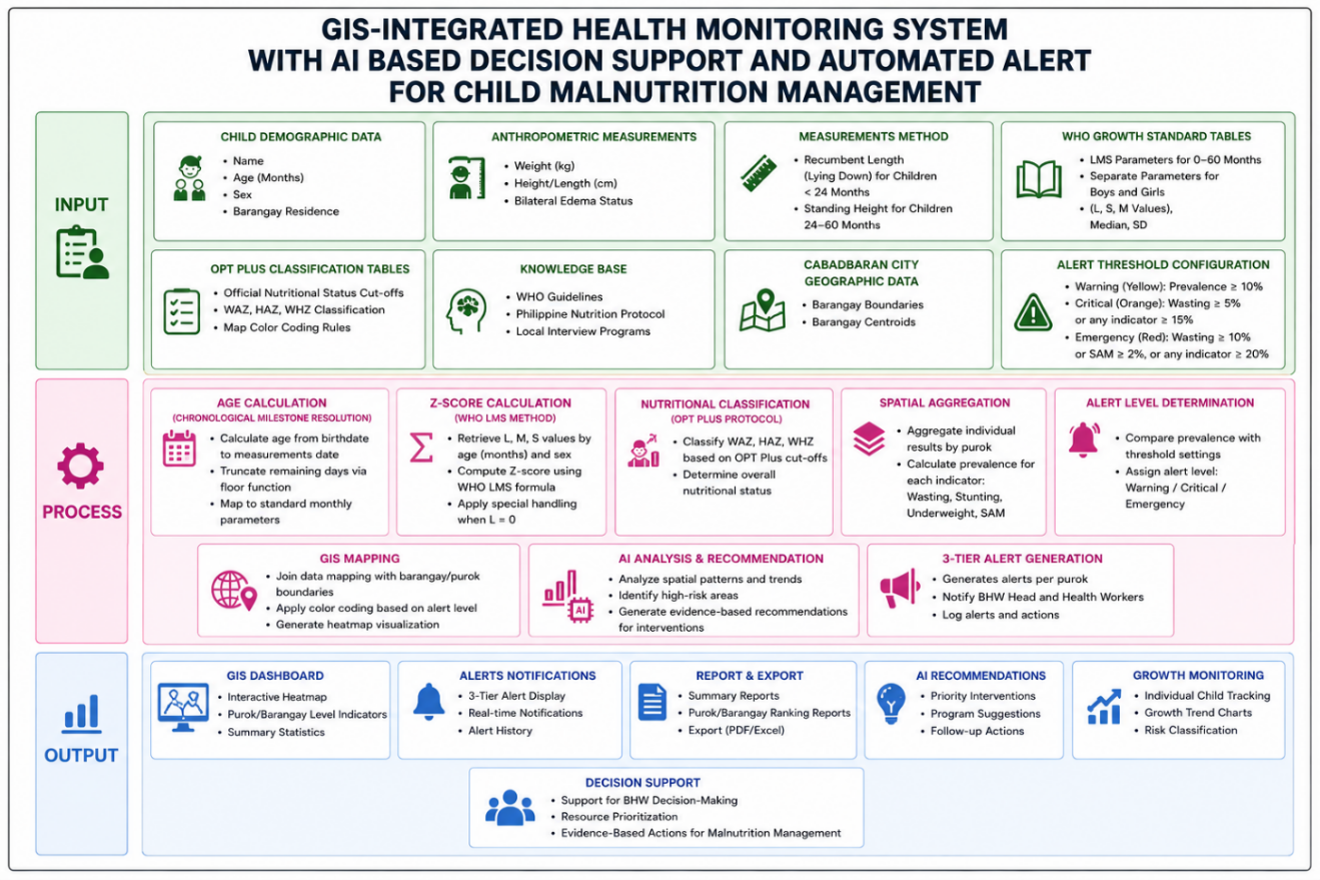
\includegraphics[width=0.95\textwidth]{ipo_model.png} 
    \caption{Input-Process-Output (IPO) Conceptual Framework of the GIS-Integrated Health Monitoring System with AI-Based Decision Support and Automated Alert for Child Malnutrition Management}
    \label{fig:ipo_model}
\end{figure}

\subsection{Input}
\label{subsec:input}
The input components of the system consist of eight categories of data:
\begin{enumerate}
    \item \textbf{Child Demographic Data} -- Name, age in months or years, sex, and barangay of residence.
    \item \textbf{Anthropometric Measurements} -- Weight in kilograms (kg), height/length in centimeters (cm), and bilateral edema status.
    \item \textbf{Measurement Method} -- Recumbent Length (lying down) for children under 24 months OR Standing Height for children 24--71 months.
    \item \textbf{WHO Growth Standard Reference Tables} -- LMS parameters for children aged 0--71 months, with separate parameters for male and female children.
    \item \textbf{OPT Plus Classification Reference Tables} -- Official nutritional status cut-offs from the National Nutrition Council Operation Timbang (OPT) Plus methodology [50].
    \item \textbf{Knowledge Base (AI Decision Support)} -- WHO guidelines, Philippine nutrition protocols, and local intervention programs (OPT Plus, supplementary feeding) for evidence-based recommendation generation [9][10].
    \item \textbf{Cabadbaran City Geographic Data} -- Boundary polygons for each barangay stored as POLYGON geometries.
    \item \textbf{Alert Threshold Configuration} -- Configurable thresholds for 3-tier alert system:
    \begin{itemize}
        \item Warning (Yellow): Prevalence \(\geq 10\%\)
        \item Critical (Orange): Wasting \(\geq 5\%\) OR Any Indicator \(\geq 15\%\)
        \item Emergency (Red): Wasting \(\geq 10\%\) OR SAM \(\geq 2\%\) OR Any Indicator \(\geq 20\%\)
    \end{itemize}
\end{enumerate}

\subsection{Process}
\label{subsec:process}
The system processes the input data through twelve sequential mechanisms:
\begin{enumerate}
    \item \textbf{Age Calculation (Chronological Milestone Resolution)} -- Calculates chronological age by finding the exact interval between date of birth and measurement date. Per NNC guidelines, any remaining days are truncated via a floor function, forcing the lookup system to utilize standard monthly parameters [50].
    \item \textbf{Height/Length Positional Adjustment} -- Applies conditional adjustments based on age and measurement method:
    \begin{itemize}
        \item Children under 24 months measured standing up: Add \(+0.7\) cm
        \item Children under 24 months measured lying down: No adjustment
        \item Children 24--71 months measured lying down: Subtract \(-0.7\) cm
        \item Children 24--71 months measured standing up: No adjustment
    \end{itemize}
    \item \textbf{Z-Score Calculation} -- Using WHO LMS parameters, calculates Weight-for-Age (WAZ), Height-for-Age (HAZ), and Weight-for-Height (WHZ) Z-scores using the Box-Cox Cole and Green method.
    \item \textbf{Clinical Priority Interception (Edema Override)} -- If bilateral edema is present, bypasses standard Z-score calculations and instantly flags the entry as an emergency case of Severe Acute Malnutrition (SAM) [50].
    \item \textbf{Nutritional Status Classification} -- Classifies each child's nutritional status based on Z-scores and OPT Plus cut-offs, enforcing overlapping edge logic (exactly \(-2.00\) is Normal) [50].
    \item \textbf{Spatial Aggregation by Barangay} -- Associates child records with specific barangays using PostGIS spatial queries (ST\_Contains, ST\_Intersects).
    \item \textbf{Heatmap and Risk Level Generation} -- Generates color-coded map with risk classifications using Leaflet.js.
    \item \textbf{Trend Analysis} -- Calculates percent change in malnutrition prevalence between time periods.
    \item \textbf{3-Tier Alert Generation} -- Monitors prevalence values and generates alerts based on configured thresholds:
    \begin{itemize}
        \item Warning (Yellow) -- Prevalence of any malnutrition type \(\geq 10\%\)
        \item Critical (Orange) -- Wasting prevalence \(\geq 5\%\) OR any indicator \(\geq 15\%\) OR \(\geq 25\%\) increase over 3 months
        \item Emergency (Red) -- Wasting prevalence \(\geq 10\%\) OR SAM \(\geq 2\%\) OR any indicator \(\geq 20\%\)
    \end{itemize}
    \item \textbf{AI-Based Decision Support} -- Analyzes Z-scores, prevalence data, and growth trends to identify barangays with elevated malnutrition risk and recommend appropriate interventions using rule-based classification and prevalence analysis [9][10][50].
    \item \textbf{Child Growth Monitoring} -- Tracks individual child growth curves against WHO standards.
    \item \textbf{Automated Report Generation} -- Produces PDF and Excel reports with AI-generated insights.
\end{enumerate}

\subsubsection{Positional Modification Factors}
\label{subsubsec:positional}
Human growth standards differentiate between recumbent length (lying down) and standing height. The system evaluates the entry using a conditional switch to reconcile errors introduced by incorrect physical field positioning during community sweeps:

\vspace{0.3cm}
\begin{longtable}{p{3.5cm} p{5cm} p{5cm}}
    \caption{Positional Modification Factors} \label{tab:positional} \\
    \toprule
    \textbf{Age Group} & \textbf{Measurement Method} & \textbf{Operational Adjustment} \\
    \midrule
    \endfirsthead
    \multicolumn{3}{c}{{\tablename\ \thetable{} -- Continued from previous page}} \\
    \toprule
    \textbf{Age Group} & \textbf{Measurement Method} & \textbf{Operational Adjustment} \\
    \midrule
    \endhead
    \midrule
    \multicolumn{3}{r}{{Continued on next page}} \\
    \endfoot
    \bottomrule
    \endlastfoot
    Under 24 months & Standing (Incorrect position) & Add +0.7 cm to value \\
    \addlinespace
    Under 24 months & Lying down (Correct position) & No adjustment (Baseline length) \\
    \addlinespace
    24 to 71 months & Lying down (Incorrect position) & Subtract -0.7 cm from value \\
    \addlinespace
    24 to 71 months & Standing (Correct position) & No adjustment (Baseline height) \\
\end{longtable}
\vspace{0.3cm}

\noindent \textbf{Algorithmic Conditional Logic:}
\begin{equation}
    \text{Adjusted Linear Measurement} = 
    \begin{cases} 
      \text{Height} + 0.7 & \text{if Age} < 24 \text{ AND Method} = \text{Standing} \\
      \text{Height} - 0.7 & \text{if Age} \geq 24 \text{ AND Method} = \text{Lying Down} \\
      \text{Height} & \text{Otherwise}
    \end{cases}
\end{equation}

\textit{Narrative Interpretation:} This adjustment standardizes all physical measurements to a common baseline, ensuring that Z-score calculations are not affected by measurement technique variations.

\subsubsection{Asymmetric Growth Mapping (LMS Pipeline)}
\label{subsubsec:lms}
The mathematical classification block implements the complete WHO Box-Cox Cole and Green calculation formula to determine precise Z-scores. This prevents skew errors by sorting records using separate parameter lookup pathways for male and female growth vectors.

\noindent \textbf{The LMS Parameters Defined:}

\vspace{0.3cm}
\begin{longtable}{p{3.5cm} p{10.5cm}}
    \caption{LMS Parameters} \label{tab:lms_params} \\
    \toprule
    \textbf{Parameter} & \textbf{Description} \\
    \midrule
    \endfirsthead
    \multicolumn{2}{c}{{\tablename\ \thetable{} -- Continued from previous page}} \\
    \toprule
    \textbf{Parameter} & \textbf{Description} \\
    \midrule
    \endhead
    \midrule
    \multicolumn{2}{r}{{Continued on next page}} \\
    \endfoot
    \bottomrule
    \endlastfoot
    L (Lambda) & Skewness coefficient (Box-Cox power transformation to normalize asymmetrical growth curves) \\
    \addlinespace
    M (Mu) & Median reference value optimized for the specific age and biological sex parameter \\
    \addlinespace
    S (Sigma) & Coefficient of variation (scaling factor mapping standard dispersion) \\
\end{longtable}
\vspace{0.3cm}

\noindent \textbf{Z-Score Formulation Matrix:}
\begin{align}
    \text{For } L \neq 0: \quad Z &= \frac{\left(\frac{X}{M}\right)^L - 1}{L \times S} \\
    \text{For } L = 0: \quad Z &= \frac{\ln\left(\frac{X}{M}\right)}{S}
\end{align}

(Where \(X\) represents the child's actual adjusted physical weight or height input)

\noindent \textbf{Gender-Specific Weight-for-Age (WAZ) Exponent Baselines:}

\vspace{0.3cm}
\begin{longtable}{p{3cm} p{2cm} p{2.5cm} p{2.5cm} p{2.5cm}}
    \caption{Gender-Specific WAZ Baselines} \label{tab:waz} \\
    \toprule
    \textbf{Milestone} & \textbf{Sex Target} & \textbf{L (Skewness)} & \textbf{M (Median Weight)} & \textbf{S (Variation)} \\
    \midrule
    \endfirsthead
    \multicolumn{5}{c}{{\tablename\ \thetable{} -- Continued from previous page}} \\
    \toprule
    \textbf{Milestone} & \textbf{Sex Target} & \textbf{L (Skewness)} & \textbf{M (Median Weight)} & \textbf{S (Variation)} \\
    \midrule
    \endhead
    \midrule
    \multicolumn{5}{r}{{Continued on next page}} \\
    \endfoot
    \bottomrule
    \endlastfoot
    Month 12 (1 Year) & Boys & -0.3521 & 9.6 kg & 0.1213 \\
    \addlinespace
    Month 12 (1 Year) & Girls & -0.3809 & 8.9 kg & 0.1281 \\
    \addlinespace
    Month 24 (2 Years) & Boys & -0.3521 & 12.2 kg & 0.1173 \\
    \addlinespace
    Month 24 (2 Years) & Girls & -0.3809 & 11.5 kg & 0.1245 \\
\end{longtable}
\vspace{0.3cm}

\noindent \textbf{Symmetrical Height-for-Age (HAZ) Linear Baselines (L = 1.0):}

\vspace{0.3cm}
\begin{longtable}{p{3cm} p{2cm} p{2.5cm} p{2.5cm} p{2.5cm}}
    \caption{Symmetrical HAZ Linear Baselines} \label{tab:haz} \\
    \toprule
    \textbf{Milestone} & \textbf{Sex Target} & \textbf{L (Skewness)} & \textbf{M (Median Height)} & \textbf{S (Variation)} \\
    \midrule
    \endfirsthead
    \multicolumn{5}{c}{{\tablename\ \thetable{} -- Continued from previous page}} \\
    \toprule
    \textbf{Milestone} & \textbf{Sex Target} & \textbf{L (Skewness)} & \textbf{M (Median Height)} & \textbf{S (Variation)} \\
    \midrule
    \endhead
    \midrule
    \multicolumn{5}{r}{{Continued on next page}} \\
    \endfoot
    \bottomrule
    \endlastfoot
    Month 12 (1 Year) & Boys & 1.0000 & 75.7 cm & 0.0354 \\
    \addlinespace
    Month 12 (1 Year) & Girls & 1.0000 & 74.0 cm & 0.0371 \\
    \addlinespace
    Month 24 (2 Years) & Boys & 1.0000 & 87.8 cm & 0.0364 \\
    \addlinespace
    Month 24 (2 Years) & Girls & 1.0000 & 86.4 cm & 0.0382 \\
\end{longtable}
\vspace{0.3cm}

\textit{Narrative Interpretation:} The LMS pipeline ensures that Z-score calculations are biologically accurate by accounting for natural growth asymmetries between sexes and age groups. The separate male/female parameter pathways prevent systematic skew errors in classification.

\subsubsection{Clinical Priority Interception (The Edema Override)}
\label{subsubsec:edema}
The system integrates an automated triage override branch. If a data enumerator flags the presence of bilateral edema during data entry, mathematical calculation loops are bypassed.

\noindent \textbf{Rationale:} Fluid accumulation artificially inflates a child's raw weight record, making statistical WAZ and WHZ computations medically invalid. The system intercepts the transaction, masks the skewed metrics, and routes the record as an emergency case of Severe Acute Malnutrition (SAM) to trigger immediate healthcare intervention protocols.

\noindent \textbf{Algorithmic Conditional Pipeline:}
\begin{verbatim}
IF Bilateral_Edema == True THEN:
    BYPASS_MATHEMATICAL_LOOPS(WAZ, HAZ, WHZ)
    SET output_nutritional_status = "Severe Acute Malnutrition (SAM)"
    EXECUTE system_alert_state(COLOR_CODE_RED, LEVEL_EMERGENCY)
    SET local_health_priority = "Immediate Emergency"
\end{verbatim}

\textit{Narrative Interpretation:} The edema override is a critical safety mechanism that prevents the system from generating false normal classifications. By skipping Z-score calculations, the system ensures that children with clinical edema are immediately routed for emergency intervention.

\subsubsection{Core Data Integrity Rules}
\label{subsubsec:integrity}
To guarantee public health surveillance accuracy across automated regional reporting boards, the platform enforces four explicit data validation parameters:

\vspace{0.3cm}
\begin{longtable}{p{3.5cm} p{10.5cm}}
    \caption{Core Data Integrity Rules} \label{tab:integrity} \\
    \toprule
    \textbf{Rule} & \textbf{Technical Description} \\
    \midrule
    \endfirsthead
    \multicolumn{2}{c}{{\tablename\ \thetable{} -- Continued from previous page}} \\
    \toprule
    \textbf{Rule} & \textbf{Technical Description} \\
    \midrule
    \endhead
    \midrule
    \multicolumn{2}{r}{{Continued on next page}} \\
    \endfoot
    \bottomrule
    \endlastfoot
    Overlapping Edge Logic & Boundary scores resting at exactly -2.00 are classified as Normal. Malnutrition alert metrics only trigger when a score falls completely past the line (e.g., -2.01 to -3.00). \\
    \addlinespace
    Drop-Day Age Factor & Micro-date calculations must drop day remainders. A record indicating 6 months and 28 days is mapped strictly onto Month 6 database parameters. \\
    \addlinespace
    Physical Adjustment Constants & Enforces a \(\pm0.7\) cm mathematical adjustment when measurement methods do not match standard recumbent length or standing height configurations for the age group. \\
    \addlinespace
    Clinical Override Clause & Intercepts calculation pipelines when bilateral edema is present, forcing an automatic SAM emergency designation. \\
\end{longtable}
\vspace{0.3cm}

\textit{Narrative Interpretation:} These four rules serve as the system's quality control framework, ensuring that all data processed by the backend maintains national surveillance standards and clinical validity.

\subsubsection{OPT Plus Classification Reference Tables}
\label{subsubsec:opt_tables}
The system handles backend database categorization mappings using these specific standard boundary parameters:

\noindent \textbf{1. Weight-for-Age (WAZ) Boundary Metrics}

\vspace{0.3cm}
\begin{longtable}{p{2.5cm} p{2.5cm} p{2.5cm} p{3.5cm}}
    \caption{WAZ Boundary Metrics} \label{tab:waz_metrics} \\
    \toprule
    \textbf{Calculated Z-Score Range} & \textbf{System Status Output} & \textbf{Dashboard Map Color} & \textbf{Public Health Priority Level} \\
    \midrule
    \endfirsthead
    \multicolumn{4}{c}{{\tablename\ \thetable{} -- Continued from previous page}} \\
    \toprule
    \textbf{Calculated Z-Score Range} & \textbf{System Status Output} & \textbf{Dashboard Map Color} & \textbf{Public Health Priority Level} \\
    \midrule
    \endhead
    \midrule
    \multicolumn{4}{r}{{Continued on next page}} \\
    \endfoot
    \bottomrule
    \endlastfoot
    Z > +2.00 & Overweight & Purple / Blue & Low Priority \\
    \addlinespace
    -2.00 \(\leq\) Z \(\leq\) +2.00 & Normal & Solid Green & Baseline \\
    \addlinespace
    -3.00 \(\leq\) Z < -2.00 & Underweight & Deep Orange & Moderate Priority \\
    \addlinespace
    Z < -3.00 & Severely Underweight & Crimson Red & High Priority \\
\end{longtable}
\vspace{0.3cm}

\noindent \textbf{2. Height-for-Age (HAZ) Boundary Metrics}

\vspace{0.3cm}
\begin{longtable}{p{2.5cm} p{2.5cm} p{2.5cm} p{3.5cm}}
    \caption{HAZ Boundary Metrics} \label{tab:haz_metrics} \\
    \toprule
    \textbf{Calculated Z-Score Range} & \textbf{System Status Output} & \textbf{Dashboard Map Color} & \textbf{Public Health Priority Level} \\
    \midrule
    \endfirsthead
    \multicolumn{4}{c}{{\tablename\ \thetable{} -- Continued from previous page}} \\
    \toprule
    \textbf{Calculated Z-Score Range} & \textbf{System Status Output} & \textbf{Dashboard Map Color} & \textbf{Public Health Priority Level} \\
    \midrule
    \endhead
    \midrule
    \multicolumn{4}{r}{{Continued on next page}} \\
    \endfoot
    \bottomrule
    \endlastfoot
    Z > +2.00 & Tall & Purple / Blue & Low Priority \\
    \addlinespace
    -2.00 \(\leq\) Z \(\leq\) +2.00 & Normal & Solid Green & Baseline \\
    \addlinespace
    -3.00 \(\leq\) Z < -2.00 & Stunted & Deep Orange & Moderate Priority \\
    \addlinespace
    Z < -3.00 & Severely Stunted & Crimson Red & Critical Chronic Threat \\
\end{longtable}
\vspace{0.3cm}

\noindent \textbf{3. Weight-for-Height/Length (WHZ) Boundary Metrics}

\vspace{0.3cm}
\begin{longtable}{p{2.5cm} p{2.5cm} p{2.5cm} p{3.5cm}}
    \caption{WHZ Boundary Metrics} \label{tab:whz_metrics} \\
    \toprule
    \textbf{Calculated Z-Score Range} & \textbf{System Status Output} & \textbf{Dashboard Map Color} & \textbf{Public Health Priority Level} \\
    \midrule
    \endfirsthead
    \multicolumn{4}{c}{{\tablename\ \thetable{} -- Continued from previous page}} \\
    \toprule
    \textbf{Calculated Z-Score Range} & \textbf{System Status Output} & \textbf{Dashboard Map Color} & \textbf{Public Health Priority Level} \\
    \midrule
    \endhead
    \midrule
    \multicolumn{4}{r}{{Continued on next page}} \\
    \endfoot
    \bottomrule
    \endlastfoot
    Z > +3.00 & Obese & Dark Purple & High Overnutrition \\
    \addlinespace
    +2.00 < Z \(\leq\) +3.00 & Overweight & Sky Blue & Moderate Overnutrition \\
    \addlinespace
    -2.00 \(\leq\) Z \(\leq\) +2.00 & Normal & Solid Green & Baseline \\
    \addlinespace
    -3.00 \(\leq\) Z < -2.00 & Wasted (Thin) & Deep Orange & High Acute Threat \\
    \addlinespace
    Z < -3.00 & Severely Wasted & Crimson Red & Emergency Immediate \\
\end{longtable}
\vspace{0.3cm}

\noindent \textbf{4. Clinical Visual Triage Indicator (Bilateral Edema)}

\vspace{0.3cm}
\begin{longtable}{p{3.5cm} p{3.5cm} p{3cm} p{3cm}}
    \caption{Clinical Visual Triage Indicator} \label{tab:triage} \\
    \toprule
    \textbf{Visual Field Observation} & \textbf{System Classification Output} & \textbf{Dashboard Map Color} & \textbf{Public Health Priority Level} \\
    \midrule
    \endfirsthead
    \multicolumn{4}{c}{{\tablename\ \thetable{} -- Continued from previous page}} \\
    \toprule
    \textbf{Visual Field Observation} & \textbf{System Classification Output} & \textbf{Dashboard Map Color} & \textbf{Public Health Priority Level} \\
    \midrule
    \endhead
    \midrule
    \multicolumn{4}{r}{{Continued on next page}} \\
    \endfoot
    \bottomrule
    \endlastfoot
    Bilateral Edema Flag = True & Severe Acute Malnutrition (SAM) & Flashing Solid Red & Immediate Emergency \\
\end{longtable}
\vspace{0.3cm}

\noindent \textbf{Summary of Framework Components}

\vspace{0.3cm}
\begin{longtable}{p{3.5cm} p{5cm} p{5cm}}
    \caption{Summary of Framework Components} \label{tab:summary_framework} \\
    \toprule
    \textbf{Component} & \textbf{Purpose} & \textbf{Key Outputs} \\
    \midrule
    \endfirsthead
    \multicolumn{3}{c}{{\tablename\ \thetable{} -- Continued from previous page}} \\
    \toprule
    \textbf{Component} & \textbf{Purpose} & \textbf{Key Outputs} \\
    \midrule
    \endhead
    \midrule
    \multicolumn{3}{r}{{Continued on next page}} \\
    \endfoot
    \bottomrule
    \endlastfoot
    Age Calculation & Standardize chronological age & Truncated months (floor function) \\
    \addlinespace
    Positional Adjustment & Correct measurement method errors & \(\pm0.7\) cm adjustment \\
    \addlinespace
    LMS Pipeline & Compute accurate Z-scores & WAZ, HAZ, WHZ values \\
    \addlinespace
    Edema Override & Bypass calculations for edematous children & SAM emergency classification \\
    \addlinespace
    Data Integrity Rules & Enforce NNC/WHO standards & Validated classification \\
    \addlinespace
    OPT Plus Tables & Map Z-scores to statuses & Nutritional status, map colors, priority levels \\
\end{longtable}
\vspace{0.3cm}

\subsection{Output}
\label{subsec:output}
The system produces seven categories of outputs:
\begin{enumerate}
    \item \textbf{Interactive Heatmap Visualization} -- Color-coded map showing malnutrition risk levels by barangay.
    \item \textbf{Child Growth Monitoring Charts} -- Individual growth curves plotted against WHO standards.
    \item \textbf{Malnutrition Trend Graphs} -- Bar charts and line charts showing cases over time.
    \item \textbf{3-Tier Early Warning Alerts} -- Dashboard notifications for barangays exceeding thresholds.
    \item \textbf{AI Recommendations} -- Evidence-based nutritional intervention suggestions grounded in WHO guidelines and NNC OPT Plus standards [9][10][50].
    \item \textbf{Risk Prioritization} -- Ranked list of high-risk children and barangays for targeted intervention.
    \item \textbf{Automated Reports} -- PDF and Excel reports summarizing malnutrition cases, incorporating AI-generated insights.
\end{enumerate}

\section{Details of the Technologies to Be Used}
\label{sec:technologies}
The system is built on the following technology stack:

\vspace{0.3cm}
\begin{longtable}{p{3cm} p{5.5cm} p{5.5cm}}
    \caption{Technology Stack} \label{tab:tech_stack} \\
    \toprule
    \textbf{Layer} & \textbf{Technology} & \textbf{Purpose} \\
    \midrule
    \endfirsthead
    \multicolumn{3}{c}{{\tablename\ \thetable{} -- Continued from previous page}} \\
    \toprule
    \textbf{Layer} & \textbf{Technology} & \textbf{Purpose} \\
    \midrule
    \endhead
    \midrule
    \multicolumn{3}{r}{{Continued on next page}} \\
    \endfoot
    \bottomrule
    \endlastfoot
    Frontend & HTML5, CSS3, JavaScript, Next.js & User interface, dashboard, data entry forms, reports and charts \\
    \addlinespace
    Backend & Python 3.9+, FastAPI & API endpoints, business logic, Z-score calculation, alert engine \\
    \addlinespace
    Database & PostgreSQL with PostGIS & Relational storage of child records and spatial storage of barangay boundaries \\
    \addlinespace
    GIS Mapping & Leaflet.js with OpenStreetMap tiles, Leaflet.heat & Interactive maps and heatmap visualization \\
    \addlinespace
    Z-Score Engine & WHO Anthro Python library & LMS-based Z-score computation \\
    \addlinespace
    AI Decision Support & Rule-based classification and prevalence analysis & Recommendation generation and risk prioritization \\
    \addlinespace
    Reporting & ReportLab (Python), jsPDF & PDF and Excel report generation \\
    \addlinespace
    Server & Apache2 on a local machine & Web server and application hosting \\
    \addlinespace
    Security & HTTPS (TLS), bcrypt/PBKDF2 & Secure transmission and password hashing \\
\end{longtable}
\vspace{0.3cm}

\noindent \textbf{Frontend.} Next.js is a React-based framework supporting server-side rendering (SSR) and static site generation (SSG), which improves initial page load times for users on slow connections. The frontend comprises the Dashboard, Map Viewer, Data Entry Forms, and Reports \& Charts modules.

\noindent \textbf{Backend.} FastAPI is a modern Python web framework chosen for its high performance, automatic API documentation, and asynchronous request handling. It is organized into seven modules: Authentication, Child Management, Health Record Processing, Nutrition Status Analyzer, Alert System, AI Decision Support, and Report Generator.

\noindent \textbf{Database.} PostgreSQL with PostGIS provides both relational data management and advanced geospatial capabilities. Spatial data types (POINT, POLYGON, MULTIPOLYGON) and functions (ST\_Contains(), ST\_Intersects(), ST\_DWithin()) support barangay boundary storage and child record geolocation. GiST indexes optimize spatial queries for real-time heatmap rendering.

\noindent \textbf{GIS Engine.} Leaflet.js is a lightweight, mobile-friendly JavaScript mapping library (approximately 42 KB minified). The Leaflet.heat plugin implements kernel density estimation using Gaussian kernels to render smooth heatmap surfaces.

\noindent \textbf{Z-Score Engine.} The WHO Anthro Python library implements the Box--Cox Cole and Green method, using gender-specific LMS parameters for children aged 0--71 months.

\section{Conceptual Framework Narrative}
\label{sec:conceptual}

\noindent \textbf{\textit{Operationalization of the National Nutrition Surveillance Logic}}

To align with the data rules established by the National Nutrition Council (NNC) and the World Health Organization (WHO), the core backend engine processes anthropometric variables through an algorithmic matrix. This pipeline applies four strict domain constraints before generating outputs to ensure data integrity and clinical accuracy in malnutrition surveillance.

\subsection{Chronological Milestone Resolution}
\label{subsec:chronological}
The system calculates a child's age by finding the exact interval between the date of birth and the measurement date. Per NNC guidelines, any remaining days are truncated using the floor function, forcing the lookup system to utilize standard monthly parameters.
For example, an infant aged 6 months and 28 days is mapped directly onto the Month 6 reference parameters, as the 28-day remainder is dropped to maintain consistency with national surveillance protocols.

\noindent \textbf{Mathematical Formula:}
\begin{equation}
    \text{Age (in months)} = \text{FLOOR}\left(\frac{\text{Measurement Date} - \text{Birth Date}}{30.4375}\right)
\end{equation}

\textit{Narrative Interpretation:} This rule ensures that all children are evaluated against the correct WHO LMS reference tables by eliminating fractional month discrepancies that could skew Z-score calculations.

\subsection{Python Backend with FastAPI}
\label{subsec:python}
Python is an interpreted, high-level, general-purpose programming language known for its simplicity and readability [26]. For this project, Python is chosen as the backend programming language due to its extensive library support for data analysis, its robust web frameworks (Flask and FastAPI), and its seamless integration with the WHO Anthro library for Z-score calculations.
FastAPI is a modern, fast web framework for building APIs with Python 3.6+ based on standard Python type hints [28]. FastAPI is chosen for its high performance, automatic API documentation, and asynchronous request handling. The backend will handle user authentication, business logic, data processing, and API endpoints that serve data to the Next.js frontend.

\subsection{Leaflet.js GIS Library}
\label{subsec:leaflet}
Leaflet.js is an open-source JavaScript library specifically designed for mobile-friendly interactive maps [29]. The library is approximately 42 KB when minified and compressed, making it fast to download even on slow internet connections. Leaflet operates on a tile-based architecture where the base map is divided into 256\(\times\)256 pixel tiles at multiple zoom levels (typically 0 to 18). For heatmap visualization, the system will use the Leaflet.heat plugin, which implements a kernel density estimation algorithm. For each malnutrition case point, the plugin applies a Gaussian kernel, and the intensity values are summed across overlapping kernels, resulting in a smooth, color-coded surface where red indicates a high density of cases.

\subsection{PostgreSQL with PostGIS Spatial Extensions}
\label{subsec:postgresql}
PostgreSQL, when extended with PostGIS, provides comprehensive geospatial capabilities through its official spatial extension module [30]. The spatial data types used in this system align with the Open Geospatial Consortium (OGC) standards and include POINT for storing barangay centroids, POLYGON for storing barangay administrative boundaries, and MULTIPOLYGON for handling non-contiguous territories. PostGIS implements spatial indexing using GiST (Generalized Search Tree) data structures. GiST indexes are highly optimized for multidimensional range queries and support advanced spatial operations such as nearest-neighbor searches (KNN), which significantly improve query performance on large geospatial datasets. The key spatial functions utilized are ST\_Contains() and ST\_Intersects(), which perform true geometric containment and intersection tests rather than relying on bounding-box approximations. Furthermore, PostGIS introduces the geography data type, which enables accurate distance calculations in meters over the Earth's spheroid using functions like ST\_DWithin() and ST\_Distance().

\subsection{WHO Anthro Z-Score Calculation}
\label{subsec:anthro}
The WHO Child Growth Standards provide the international standard for assessing child growth from birth to 5 years of age [31]. The LMS method summarizes the distribution of growth measurements at each age using three parameters: L (Lambda) for Box-Cox transformation power, M (Mu) for the median value, and S (Sigma) for the coefficient of variation. For a given child's measurement X, age, and sex, the Z-score is calculated using the Box-Cox Cole and Green method. The proposed system will use the WHO Anthro software and the Python anthro package for accurate Z-score calculation [32].

\subsection{Next.js Framework}
\label{subsec:nextjs}
Next.js is a React-based web development framework created by Vercel [33]. Unlike traditional React applications that render entirely on the client side, Next.js supports server-side rendering (SSR) and static site generation (SSG). For the proposed system, Next.js provides faster initial page load times, which is particularly beneficial for users with slow internet connections, and built-in API routes allowing the backend Python API to be served from the same domain.

\subsection{AI-Based Decision Support}
\label{subsec:aidss}
The system integrates AI-based decision support that automatically analyzes input data and generates intelligent recommendations for child nutrition interventions [9][10]. The decision support system uses rule-based classification and prevalence analysis to identify barangays and puroks with elevated malnutrition risk and recommend appropriate actions.

\noindent \textbf{How It Works:}
\begin{enumerate}
    \item \textbf{Data Analysis} -- The system automatically analyzes child records, Z-scores, and nutritional status from entered data.
    \item \textbf{Prevalence Calculation} -- Computes malnutrition prevalence for each barangay and purok based on OPT Plus standards [50].
    \item \textbf{Risk Identification} -- Identifies barangays and puroks with high cases of wasting, stunting, underweight, or SAM.
    \item \textbf{Automatic Decision Support} -- Generates automatic recommendations based on prevalence thresholds:
    \begin{itemize}
        \item Warning (Yellow): Prevalence \(\geq 10\%\) \(\rightarrow\) Schedule follow-up assessment
        \item Critical (Orange): Wasting \(\geq 5\%\) OR Any Indicator \(\geq 15\%\) \(\rightarrow\) Conduct supplementary feeding
        \item Emergency (Red): Wasting \(\geq 10\%\) OR SAM \(\geq 2\%\) \(\rightarrow\) Immediate intervention required
    \end{itemize}
    \item \textbf{Recommendation Output} -- Displays automatic recommendations on the dashboard:
    \begin{itemize}
        \item ``Barangay X is in need of supplementary feeding program''
        \item ``Purok Y has high wasting cases -- prioritize intervention''
        \item ``Schedule immediate nutrition assessment for Barangay Z''
    \end{itemize}
\end{enumerate}

\subsection{Integration Architecture}
\label{subsec:integration}
The technologies integrate through a RESTful API architecture. The browser (Next.js frontend) makes HTTP requests to the Python backend (FastAPI). The backend queries the PostgreSQL database (including spatial queries using PostGIS extensions), calls the WHO Anthro Python library for Z-score calculations, and applies rule-based classification and prevalence analysis for AI-based decision support based on NNC OPT Plus Guidelines. The backend returns JSON responses to the frontend, which renders data using Leaflet.js for maps and Chart.js for graphs.

\section{How the Project Will Work}
\label{sec:how_project_works}
The operational workflow of the system follows a twelve-step sequence from data entry to report generation:
\begin{enumerate}
    \item A health worker logs in through the Next.js frontend; credentials are sent via HTTPS POST to the Python backend.
    \item The backend queries the PostgreSQL User table and returns a JWT token to the frontend.
    \item The health worker enters the child's weight, height, and age; the frontend sends the data to the /api/child/add endpoint.
    \item The backend calculates Z-scores using the WHO Anthro Python library and stores the results in the Health\_Record and Nutrition\_Status tables.
    \item The backend triggers recomputation of barangay prevalence and checks alert thresholds.
    \item If an alert condition is met, an Alert record is created and a badge is displayed on the dashboard.
    \item The backend forwards Z-scores and nutritional status to the AI Decision Support Module.
    \item The AI Module retrieves relevant knowledge (WHO guidelines, local protocols) and generates recommendations.
    \item The AI Module prioritizes high-risk cases and stores recommendations in the database.
    \item The frontend requests heatmap data from /api/gis/heatmap; the backend executes a PostGIS spatial query on the Barangay table.
    \item The backend returns GeoJSON data, which Leaflet.js renders as a heatmap overlay.
    \item The frontend requests AI recommendations and displays them on the dashboard and in generated reports.
\end{enumerate}
This workflow ensures that every child record entered by a Barangay Nutrition Scholar or Barangay Health Worker is immediately processed, classified, spatially aggregated, and evaluated for alerting and decision support, transforming manual paper-based OPT Plus records into a near real-time digital monitoring system.

\clearpage

% ==========================================
% CHAPTER IV - METHODOLOGY
% ==========================================
\chapter{Methodology}
\label{chap:methodology}

This chapter presents the systematic approach used to develop the GIS-Based Health Monitoring System for mapping malnutrition cases among children in Cabadbaran City. It describes the research design, requirements analysis, system design, development methodology, testing procedures, deployment strategy, and evaluation plan.

\section{Planning}
\label{sec:planning}
This study employs a descriptive-developmental research design combined with the Agile software development methodology. The descriptive component involves gathering and analyzing the current malnutrition data collection and monitoring practices of barangay health workers in Cabadbaran City through document reviews and informal interviews. The developmental component focuses on designing, building, and evaluating a GIS-based web application with AI Decision Support that addresses the identified gaps in the existing process.
The choice of Agile methodology is justified by the following factors. First, iterative delivery allows the research team to produce functional system increments after each sprint, enabling continuous feedback from stakeholders. Second, flexibility accommodates evolving requirements as users interact with early versions of the system. Third, risk reduction is achieved by prioritizing core features like the malnutrition heatmap and data entry in early sprints. Finally, user-centered design is facilitated through frequent demonstrations and feedback sessions with intended users.

\subsection{Technology Acceptance Model (TAM) Research Framework}
\label{subsec:tam_research}
To ensure the system is not only technically functional but also practically adopted by its intended users, this study is anchored on the Technology Acceptance Model (TAM) as its primary theoretical framework. TAM, originally developed by Davis [38], posits that an individual's behavioral intention to use a technology is primarily determined by two key perceptions: Perceived Usefulness (PU) and Perceived Ease of Use (PEOU).
Perceived Usefulness refers to ``the degree to which a person believes that using a particular system would enhance their job performance'' [38]. In this study, PU reflects the extent to which barangay health workers (BHWs), Barangay Admins (BHW Heads), and Super Admins (CHO) believe that the GIS-Integrated Health Monitoring System with AI Decision Support will improve their ability to track, monitor, and report child malnutrition cases in Cabadbaran City.
Perceived Ease of Use refers to ``the degree to which a person believes that using a particular system would be free of effort'' [38]. For this study, PEOU captures BHWs' perceptions of how simple and intuitive the system is to learn and operate, particularly given their varying levels of technical literacy and limited prior exposure to GIS-based health information systems and AI-powered tools.

\noindent \textbf{\textit{Extended TAM Constructs for This Study}}

Given the specific context of Barangay Health Workers in Cabadbaran City, this study adopts an extended TAM framework that incorporates additional variables relevant to the Philippine public health setting:

\vspace{0.3cm}
\begin{longtable}{p{3.5cm} p{5.5cm} p{5cm}}
    \caption{Extended TAM Constructs} \label{tab:tam_constructs} \\
    \toprule
    \textbf{Construct} & \textbf{Definition} & \textbf{Application in This Study} \\
    \midrule
    \endfirsthead
    \multicolumn{3}{c}{{\tablename\ \thetable{} -- Continued from previous page}} \\
    \toprule
    \textbf{Construct} & \textbf{Definition} & \textbf{Application in This Study} \\
    \midrule
    \endhead
    \midrule
    \multicolumn{3}{r}{{Continued on next page}} \\
    \endfoot
    \bottomrule
    \endlastfoot
    Perceived Usefulness (PU) & Degree to which user believes system enhances job performance [38]. & BHWs' belief that the GIS system improves malnutrition monitoring and reporting efficiency. \\
    \addlinespace
    Perceived Ease of Use (PEOU) & Degree to which user believes system is free of effort [38]. & BHWs' perception of how intuitive the heatmap, data entry, and report generation features are. \\
    \addlinespace
    Facilitating Conditions & Availability of organizational and technical infrastructure to support system use [48]. & Access to computers, internet, electricity, and technical support at barangay health centers. \\
    \addlinespace
    Self-Efficacy & User's confidence in ability to use the technology [44]. & BHWs' belief in their capacity to navigate the GIS-based system effectively. \\
    \addlinespace
    System Quality & Reliability, accuracy, and responsiveness of the system [46]. & System's ability to generate accurate heatmaps, Z-scores, and alerts without errors. \\
    \addlinespace
    Perceived Reliability of AI Recommendations & Degree to which user trusts and relies on AI-generated suggestions [9][10]. & BHWs' confidence in the accuracy and usefulness of AI-generated nutritional recommendations. \\
    \addlinespace
    Behavioral Intention (BI) & User's intention to adopt and continue using the system. & BHWs' and health officers' willingness to use the system for routine malnutrition monitoring. \\
    \addlinespace
    Actual System Use (AU) & Actual frequency and extent of system usage. & System log data tracking login frequency, data entry volume, and report generation. \\
\end{longtable}
\vspace{0.3cm}

\noindent \textbf{\textit{Research Hypotheses}}

Based on the extended TAM framework, the following hypotheses are proposed for this study:

\vspace{0.3cm}
\begin{longtable}{p{2cm} p{12cm}}
    \caption{Research Hypotheses} \label{tab:hypotheses} \\
    \toprule
    \textbf{Hypothesis} & \textbf{Statement} \\
    \midrule
    \endfirsthead
    \multicolumn{2}{c}{{\tablename\ \thetable{} -- Continued from previous page}} \\
    \toprule
    \textbf{Hypothesis} & \textbf{Statement} \\
    \midrule
    \endhead
    \midrule
    \multicolumn{2}{r}{{Continued on next page}} \\
    \endfoot
    \bottomrule
    \endlastfoot
    H1 & Perceived Ease of Use has a positive effect on Perceived Usefulness of the GIS-Based Health Monitoring System \\
    \addlinespace
    H2 & Perceived Usefulness has a positive effect on Behavioral Intention to use the system \\
    \addlinespace
    H3 & Perceived Ease of Use has a positive effect on Behavioral Intention to use the system \\
    \addlinespace
    H4 & Facilitating Conditions have a positive effect on Perceived Ease of Use \\
    \addlinespace
    H5 & Self-Efficacy has a positive effect on Perceived Ease of Use \\
    \addlinespace
    H6 & System Quality has a positive effect on Perceived Usefulness \\
    \addlinespace
    H7 & Behavioral Intention has a positive effect on Actual System Use \\
    \addlinespace
    H8 & Perceived Reliability of AI Recommendations has a positive effect on Perceived Usefulness of the system \\
\end{longtable}
\vspace{0.3cm}

\noindent \textbf{\textit{Research Model}}

\begin{figure}[H]
    \centering
    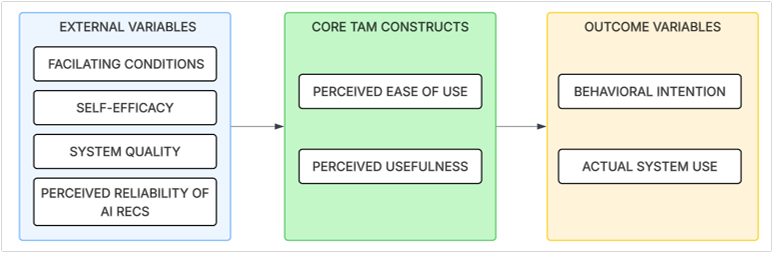
\includegraphics[width=0.85\textwidth]{tam_model.png} 
    \caption{Extended Technology Acceptance Model for the GIS-Integrated Child Nutrition Monitoring System With AI-Based Decision Support And Automated Alerts For Malnutrition Management}
    \label{fig:tam_model}
\end{figure}

\noindent \textbf{\textit{Justification for TAM Adoption}}

The adoption of TAM in this study is justified by several factors:
\begin{enumerate}
    \item \textbf{Empirical Validation:} TAM has been extensively validated across diverse healthcare contexts and user populations, including systematic reviews confirming its effectiveness in health informatics [23][39][40][41].
    \item \textbf{Contextual Relevance:} TAM has been successfully applied in Philippine health informatics research, including studies on electronic health records and electronic medical records [44][45].
    \item \textbf{GIS Integration:} Recent research has validated the application of TAM in GIS adoption, demonstrating that perceived usefulness and perceived ease of use significantly affect GIS adoption in public sector organizations [46].
    \item \textbf{Child Health Focus:} TAM has been applied specifically to child health and nutrition surveillance applications, providing a validated framework for evaluating nutrition-focused digital health interventions [47].
    \item \textbf{AI Integration:} Recent studies have extended TAM to include AI-specific constructs such as trust and perceived reliability of AI recommendations, which are critical for user acceptance of AI-powered health systems [9][10].
    \item \textbf{Practical Utility:} TAM's constructs directly translate to actionable design recommendations. By measuring PU and PEOU, researchers can identify specific areas for system improvement before full deployment.
\end{enumerate}

\subsection{Development Methodology (Agile Sprints)}
\label{subsec:agile}
The development is divided into five sprints, each lasting two weeks (total 10 weeks, plus 2 weeks for testing and deployment).

\begin{figure}[H]
    \centering
    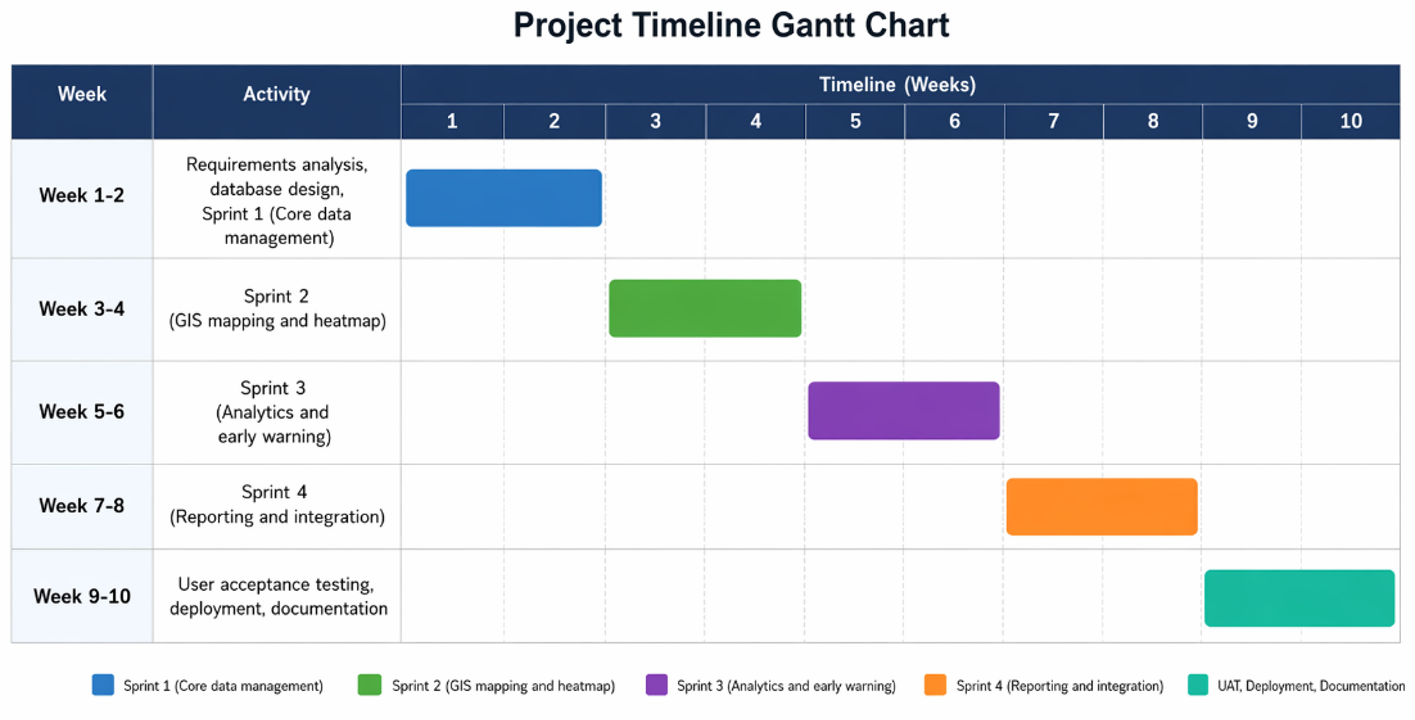
\includegraphics[width=0.9\textwidth]{gantt_chart.png}
    \caption{Project Timeline Gantt Chart}
    \label{fig:gantt_chart}
\end{figure}

\vspace{0.3cm}
\begin{longtable}{p{3cm} p{11cm}}
    \caption{Agile Sprints Timeline} \label{tab:agile_timeline} \\
    \toprule
    \textbf{Week} & \textbf{Activity} \\
    \midrule
    \endfirsthead
    \multicolumn{2}{c}{{\tablename\ \thetable{} -- Continued from previous page}} \\
    \toprule
    \textbf{Week} & \textbf{Activity} \\
    \midrule
    \endhead
    \midrule
    \multicolumn{2}{r}{{Continued on next page}} \\
    \endfoot
    \bottomrule
    \endlastfoot
    Week 1-2 & Requirements analysis, database design, Sprint 1 (Core data management) \\
    \addlinespace
    Week 3-4 & Sprint 2 (GIS mapping and heatmap) \\
    \addlinespace
    Week 5-6 & Sprint 3 (Analytics and early warning) \\
    \addlinespace
    Week 7-8 & Sprint 4 (AI Decision Support module development) \\
    \addlinespace
    Week 9-10 & Sprint 5 (Reporting and integration) \\
    \addlinespace
    Week 11-12 & User acceptance testing, deployment, documentation \\
\end{longtable}
\vspace{0.3cm}

\textbf{Sprint 1: Core Data Management (Weeks 1-2)} -- Establish PostgreSQL database with PostGIS extensions, Python backend with FastAPI and API endpoints, Next.js frontend with basic CRUD forms, and user authentication (JWT-based).

\textbf{Sprint 2: GIS Mapping and Heatmap (Weeks 3-4)} -- Leaflet.js map with Cabadbaran City barangay boundaries, geocoding of child records to barangay centroids using PostGIS spatial queries, heatmap layer showing malnutrition density, and click-for-details functionality.

\textbf{Sprint 3: Analytics and Early Warning (Weeks 5-6)} -- Dashboard with line chart showing malnutrition trends over months, bar chart comparing cases per barangay, early warning alert logic (Python backend) with 3-tier system (Warning, Critical, Emergency), and alert list viewable by City Program Nutrition Officer.

\textbf{Sprint 4: AI Decision Support (Weeks 7-8)} -- Development of AI Decision Support Module including Recommendation Engine, Risk Prioritization, and Rule-Based Classification Engine based on NNC OPT Plus Guidelines [50].

\textbf{Sprint 5: Reporting and Final Integration (Weeks 9-10)} -- Automated PDF (ReportLab) and Excel report generator, incorporation of AI recommendations into reports, user manual with in-system tooltips, full integration of all modules into single web application, and deployment on local Apache2 server.

\subsection{Development Platform and Technology Stack}
\label{subsec:dev_stack}
The system will be developed using:
\begin{itemize}
    \item \textbf{Frontend:} HTML5, CSS3, JavaScript, Next.js [33]
    \item \textbf{GIS Mapping:} Leaflet.js with OpenStreetMap tiles [29]
    \item \textbf{Backend:} Python with FastAPI [28]
    \item \textbf{Database:} PostgreSQL with PostGIS spatial extensions [30]
    \item \textbf{Z-Score Calculation:} WHO Anthro Python library [32]
    \item \textbf{AI Decision Support:} Rule-based classification and prevalence analysis using NNC OPT Plus Guidelines [50]
    \item \textbf{Reporting:} ReportLab (Python) or jsPDF [34][35]
    \item \textbf{Server:} Apache2 on local server [36]
    \item \textbf{Security:} HTTPS, bcrypt/PBKDF2 for password hashing [37][38]
\end{itemize}

\section{Requirements Specification}
\label{sec:requirements}
Requirements were gathered through three primary methods: a review of existing documents including Operation Timbang forms, nutrition reports, and barangay health records; informal interviews with three barangay health workers and the City Program Nutrition Officer, who is under the City Health Office of Cabadbaran City; and direct observation of current data recording and reporting practices at the Barangay Health Center.

\subsection{Respondents of the Study}
\label{subsec:respondents}
The respondents of this study consist of the following participants:

\vspace{0.3cm}
\begin{longtable}{p{3.5cm} p{7cm} p{3cm}}
    \caption{Respondents of the Study} \label{tab:respondents} \\
    \toprule
    \textbf{User Role} & \textbf{Description} & \textbf{Estimated Number} \\
    \midrule
    \endfirsthead
    \multicolumn{3}{c}{{\tablename\ \thetable{} -- Continued from previous page}} \\
    \toprule
    \textbf{User Role} & \textbf{Description} & \textbf{Estimated Number} \\
    \midrule
    \endhead
    \midrule
    \multicolumn{3}{r}{{Continued on next page}} \\
    \endfoot
    \bottomrule
    \endlastfoot
    Barangay Health Workers (BHWs) & Frontline health workers responsible for data collection during Operation Timbang (OPT) & 15-20 BHWs \\
    \addlinespace
    Barangay Admin / BHW Head & Health officers assigned to specific barangays who manage BHWs and puroks & 5-10 Barangay Admins \\
    \addlinespace
    Super Admin (CHO / City Program Nutrition Office) & City Program Nutrition Officer responsible for nutrition programs under the City Health Office, with city-wide oversight & 1-2 CHO/Nutrition Staff \\
    \addlinespace
    System Administrator & IT personnel responsible for technical system maintenance & 1-2 IT staff \\
\end{longtable}
\vspace{0.3cm}

\textit{Sampling Technique:} The study will employ purposive sampling to select respondents directly involved in monitoring and data collection on child malnutrition in Cabadbaran City. This sampling technique is appropriate as it targets individuals with specific knowledge and experience relevant to the system being developed.

\subsection{Functional Requirements}
\label{subsec:functional}
The following functional requirements were identified:
\begin{enumerate}
    \item The system shall allow barangay health workers to add, edit, delete, and view child records including name, age, weight, height/length, barangay, bilateral edema status, and measurement method.
    \item The system shall display malnutrition cases on an interactive map of Cabadbaran City with zoom and click-for-details functionality.
    \item The system shall generate a color-coded heatmap showing areas with high concentration of malnutrition cases.
    \item The system shall plot individual child's weight-for-age and height-for-age against WHO growth standards.
    \item The system shall show statistical graphs such as bar charts and line charts comparing malnutrition cases across months and barangays.
    \item The system shall automatically flag barangays where malnutrition cases exceed configurable 3-tier thresholds (Warning, Critical, Emergency).
    \item The system shall generate PDF or Excel reports for a selected barangay or for the entire city.
    \item The system shall provide secure user authentication for health workers and administrators.
    \item The system shall provide AI-generated recommendations for nutritional interventions based on child's Z-scores, nutritional status, and growth trends using rule-based classification and prevalence analysis based on NNC OPT Plus Guidelines.
    \item The system shall prioritize high-risk children and barangays based on malnutrition severity and prevalence.
    \item The system shall enforce OPT Plus data integrity rules including overlapping edge logic, drop-day age factor, and physical adjustment constants as specified in the NNC OPT Plus Guidelines [50].
    \item The system shall implement an edema override that bypasses Z-score calculations when bilateral edema is flagged and automatically classifies as Severe Acute Malnutrition (SAM).
\end{enumerate}

\subsection{Non-Functional Requirements}
\label{subsec:nonfunctional}
The non-functional requirements are as follows:
\begin{itemize}
    \item \textbf{Usability.} The system shall be usable by barangay health workers with basic computer literacy.
    \item \textbf{Performance.} The map and heatmap shall load within five seconds on a standard DSL connection.
    \item \textbf{Availability.} The web application shall be accessible during health center hours with ninety-nine percent uptime.
    \item \textbf{Security.} All data transmissions shall be over HTTPS and user passwords shall be hashed.
    \item \textbf{Scalability.} The database shall support at least ten thousand child records.
    \item \textbf{Data Integrity.} The system shall enforce OPT Plus data rules including overlapping edge logic (\(\pm2.00\) is Normal), drop-day age factor (truncate days), and physical adjustment constants (+0.7 cm / -0.7 cm) as specified in the NNC OPT Plus Guidelines [49].
    \item \textbf{Gender-Specific Parameters.} The system shall use separate LMS parameter lookup pathways for male and female growth vectors.
\end{itemize}

\subsection{Hardware Requirements}
\label{subsec:hardware}
The following hardware specifications are required to ensure the optimal performance, reliability, and security of the GIS-Integrated Child Nutrition Monitoring System within the City Health Office network.

\vspace{0.3cm}
\begin{longtable}{p{3cm} p{4cm} p{4cm} p{3cm}}
    \caption{Hardware Requirements} \label{tab:hardware} \\
    \toprule
    \textbf{Hardware Component} & \textbf{Minimum Specification} & \textbf{Recommended Specification} & \textbf{Purpose} \\
    \midrule
    \endfirsthead
    \multicolumn{4}{c}{{\tablename\ \thetable{} -- Continued from previous page}} \\
    \toprule
    \textbf{Hardware Component} & \textbf{Minimum Specification} & \textbf{Recommended Specification} & \textbf{Purpose} \\
    \midrule
    \endhead
    \midrule
    \multicolumn{4}{r}{{Continued on next page}} \\
    \endfoot
    \bottomrule
    \endlastfoot
    Server (Local Machine) & Intel Core i5 (8th Gen or higher), 8 GB RAM, 500 GB HDD & Intel Core i7, 16 GB RAM, 1 TB SSD & Hosts the Apache2 web server, Python FastAPI backend, and PostgreSQL/PostGIS database. \\
    \addlinespace
    Client Workstations & Intel Core i3, 4 GB RAM, 500 MB free storage & Intel Core i5, 8 GB RAM, 1 GB free storage & Used by Barangay Health Workers and Admins to access the web system, input data, and view maps. \\
    \addlinespace
    Network Infrastructure & Standard DSL connection (5 Mbps) & Fiber internet connection (10 Mbps or higher) & Ensures stable connectivity for data syncing, map rendering (Leaflet.js), and report generation. \\
    \addlinespace
    Display Monitor & 1366 x 768 resolution & 1920 x 1080 resolution (Full HD) & Essential for viewing detailed GIS heatmaps, data entry forms, and statistical charts clearly. \\
    \addlinespace
    Backup Storage & 1 TB External Hard Drive & 2 TB Network Attached Storage (NAS) & Used for regular database backups (PostgreSQL) and system logs. \\
\end{longtable}
\vspace{0.3cm}

The server is designed to operate locally within the City Health Office to ensure data privacy and security, while client workstations require only a web browser and stable internet connection.

\subsection{Software Requirements}
\label{subsec:software}
The system is built using a modern technology stack that ensures high performance, spatial data management, and responsive user interfaces. The following software requirements are necessary for the development and deployment of the system.

\vspace{0.3cm}
\begin{longtable}{p{3cm} p{5cm} p{6cm}}
    \caption{Software Requirements} \label{tab:software} \\
    \toprule
    \textbf{Layer} & \textbf{Software / Technology} & \textbf{Version / Purpose} \\
    \midrule
    \endfirsthead
    \multicolumn{3}{c}{{\tablename\ \thetable{} -- Continued from previous page}} \\
    \toprule
    \textbf{Layer} & \textbf{Software / Technology} & \textbf{Version / Purpose} \\
    \midrule
    \endhead
    \midrule
    \multicolumn{3}{r}{{Continued on next page}} \\
    \endfoot
    \bottomrule
    \endlastfoot
    Operating System (Server) & Ubuntu Server or Windows Server & 20.04 LTS or higher. Hosts the backend application, database, and web server. \\
    \addlinespace
    Operating System (Client) & Windows 10 / 11, macOS, or Linux & Latest stable version. Used by BHWs and Admins to access the system via web browsers. \\
    \addlinespace
    Web Browser & Google Chrome, Mozilla Firefox, Microsoft Edge & Latest stable version. Required to access the frontend interface, Leaflet.js maps, and dashboards. \\
    \addlinespace
    Frontend Framework & Next.js (React-based) & v14 or higher. Provides server-side rendering and a responsive user interface. \\
    \addlinespace
    Backend Framework & Python with FastAPI & Python 3.9+, FastAPI 0.100+. Handles API endpoints, business logic, and Z-score calculations. \\
    \addlinespace
    Database & PostgreSQL with PostGIS extension & PostgreSQL 14+, PostGIS 3.0+. Stores relational data and spatial data (barangay boundaries). \\
    \addlinespace
    Web Server & Apache2 & v2.4 or higher. Serves the frontend and manages reverse proxy for the backend API. \\
    \addlinespace
    GIS Library & Leaflet.js with Leaflet.heat plugin & v1.9.4 or higher. Renders interactive maps and heatmap visualizations. \\
    \addlinespace
    Z-Score Library & WHO Anthro (Python package) & Latest version. Computes WAZ, HAZ, and WHZ based on WHO LMS parameters. \\
    \addlinespace
    Reporting Library & ReportLab (Python) / jsPDF & Latest version. Generates automated PDF and Excel reports. \\
    \addlinespace
    Development Tools & Visual Studio Code, Git, pgAdmin & Latest version. Used for coding, version control, and database management. \\
    \addlinespace
    Security & OpenSSL (HTTPS/TLS), bcrypt & Latest version. Ensures secure data transmission and hashed password storage. \\
\end{longtable}
\vspace{0.3cm}

All software used in the system are open-source and widely supported, which minimizes licensing costs for the LGU. PostgreSQL with PostGIS is specifically chosen to handle the complex spatial queries required for the barangay-level heatmap and risk analysis.

\section{Analysis}
\label{sec:analysis}
This section presents the statistical analysis and evaluation methods used to process the data gathered from the respondents and to evaluate the performance of the developed system. The analysis is divided into two main parts: (1) the statistical treatment of survey data to validate the extended Technology Acceptance Model (TAM), and (2) the accuracy and performance metrics used to evaluate the GIS and alert system features.
To test the hypotheses proposed in Section 4.1.1, Pearson correlation analysis will be conducted to determine the relationships between TAM constructs. Additionally, multiple regression analysis will be performed to identify which factors significantly predict Behavioral Intention (BI) and Actual System Use (AU).
The regression models for the TAM constructs are as follows:
\begin{align}
    \text{BI} &= \beta_0 + \beta_1(\text{PU}) + \beta_2(\text{PEOU}) + \epsilon \\
    \text{AU} &= \beta_0 + \beta_1(\text{BI}) + \epsilon \\
    \text{PU} &= \beta_0 + \beta_1(\text{PEOU}) + \beta_2(\text{SQ}) + \beta_3(\text{PRAI}) + \epsilon \\
    \text{PEOU} &= \beta_0 + \beta_1(\text{FC}) + \beta_2(\text{SE}) + \epsilon
\end{align}

Where:
\begin{itemize}
    \item BI = Behavioral Intention
    \item AU = Actual System Use
    \item PU = Perceived Usefulness
    \item PEOU = Perceived Ease of Use
    \item FC = Facilitating Conditions
    \item SE = Self-Efficacy
    \item SQ = System Quality
    \item PRAI = Perceived Reliability of AI Recommendations
    \item \(\beta\) = Regression coefficients
    \item \(\epsilon\) = Error term
\end{itemize}

\subsection{Likert Scale and Interpretation}
\label{subsec:likert}
\vspace{0.3cm}
\begin{longtable}{p{2cm} p{4cm} p{5cm}}
    \caption{Likert Scale and Interpretation} \label{tab:likert} \\
    \toprule
    \textbf{Scale} & \textbf{Rating} & \textbf{Interpretation} \\
    \midrule
    \endfirsthead
    \multicolumn{3}{c}{{\tablename\ \thetable{} -- Continued from previous page}} \\
    \toprule
    \textbf{Scale} & \textbf{Rating} & \textbf{Interpretation} \\
    \midrule
    \endhead
    \midrule
    \multicolumn{3}{r}{{Continued on next page}} \\
    \endfoot
    \bottomrule
    \endlastfoot
    5 & Strongly Agree & Excellent \\
    \addlinespace
    4 & Agree & Good \\
    \addlinespace
    3 & Neutral & Fair \\
    \addlinespace
    2 & Disagree & Poor \\
    \addlinespace
    1 & Strongly Disagree & Very Poor \\
\end{longtable}
\vspace{0.3cm}

\begin{equation}
    \bar{x} = \frac{\Sigma (f_i \times w_i)}{N}
\end{equation}

Where:
\begin{itemize}
    \item \(\bar{x}\) = weighted mean
    \item \(f_i\) = frequency of responses for each scale value
    \item \(w_i\) = weight value (1 to 5)
    \item \(N\) = total number of respondents
\end{itemize}

Example: If 5 respondents rate a feature as 5, 3 rate it as 4, and 2 rate it as 3, the weighted mean is \((5\times5 + 3\times4 + 2\times3) \div 10 = (25 + 12 + 6) \div 10 = 43 \div 10 = 4.3\) (Agree/Good).

\subsection{Acceptance Criterion}
\label{subsec:acceptance}
The system is acceptable if:
\begin{enumerate}
    \item The overall weighted mean across all ISO 25010 characteristics is 4.0 (Agree) or higher.
    \item The weighted mean for Perceived Usefulness (PU) is 4.0 (Agree) or higher.
    \item The weighted mean for Perceived Ease of Use (PEOU) is 4.0 (Agree) or higher.
    \item The weighted mean for Behavioral Intention (BI) is 4.0 (Agree) or higher.
    \item The weighted mean for Perceived Reliability of AI Recommendations (PRAI) is 4.0 (Agree) or higher.
\end{enumerate}

\subsection{Percentage Accuracy for GIS Features}
\label{subsec:accuracy}
\begin{equation}
    \text{Accuracy} = \left(1 - \frac{|\text{Expected} - \text{Actual}|}{\text{Expected}}\right) \times 100\%
\end{equation}
Where Expected is the number of children manually verified in a barangay, and Actual is the count displayed by the system. An accuracy of 95\% or higher is required for the heatmap feature to be considered reliable.

\section{System Design}
\label{sec:system_design}
This section presents the architectural and structural design of the GIS-Integrated Child Nutrition Monitoring System with AI-Based Decision Support. The system design illustrates how the system's components interact with external entities, how data flows through the internal processes, how the database is structured, and how the system is deployed within the City Health Office network.
The design is organized into six sub-sections: the Context Diagram (Level 0 DFD) which provides the highest-level overview of the system; the Data Flow Diagram (DFD) which illustrates the functional processes; the UML Use Case Diagram which defines the interactions between user roles and system features; the Entity Relationship Diagram (ERD) which models the database structure; the System Architecture which describes the layered technical infrastructure; and the Algorithm Design which details the computational logic for Z-score calculation, classification, and alert generation.

\subsection{Context Diagram}
\label{subsec:context}
The Context Diagram (also known as Level 0 DFD) provides a high-level overview of the GIS-Integrated Health Monitoring System for child malnutrition cases in Cabadbaran City. It represents the entire system as a single process and shows its interactions with external entities.

\begin{figure}[H]
    \centering
    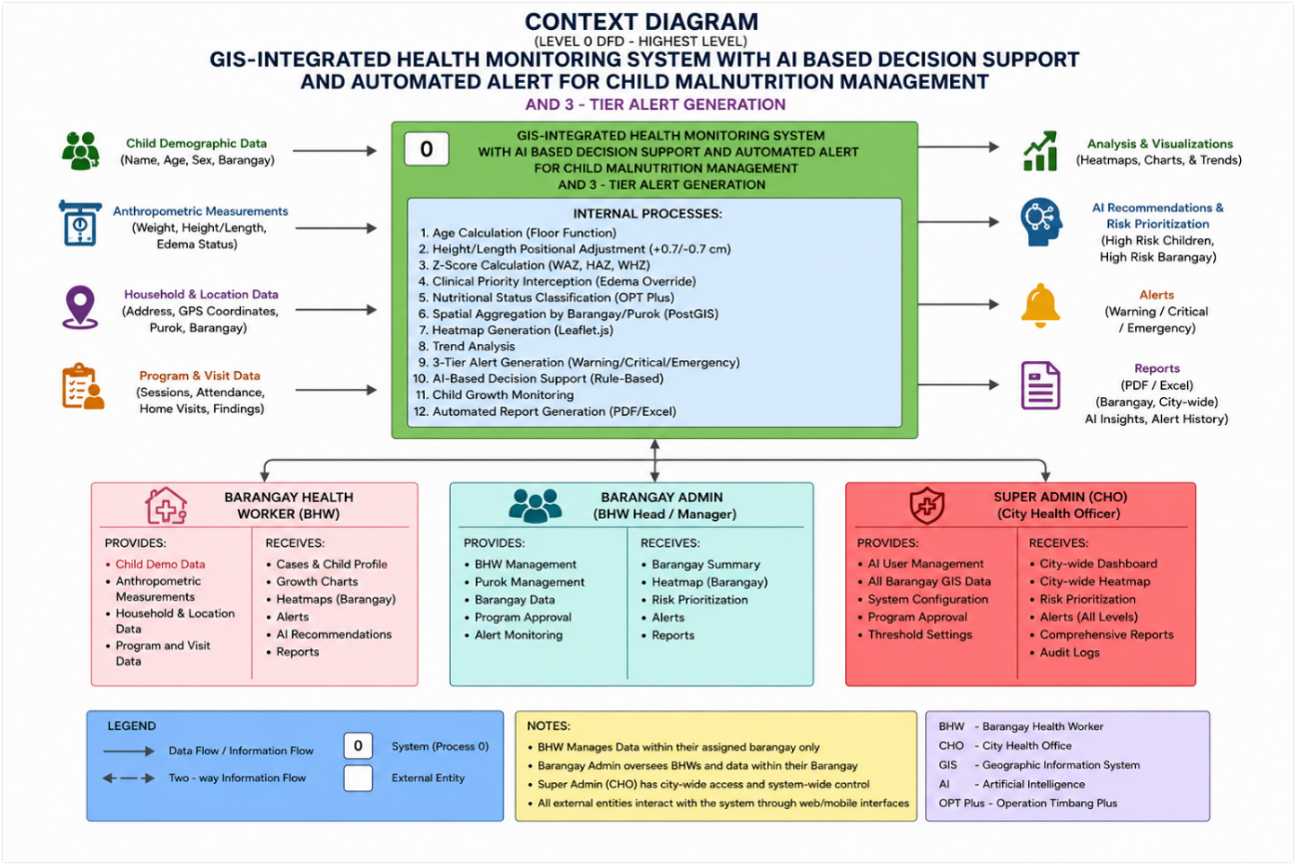
\includegraphics[width=0.95\textwidth]{context_diagram.png}
    \caption{Context Diagram of the GIS-Integrated Health Monitoring System with AI Based Decision Support and Automated Alert for Child Malnutrition Management}
    \label{fig:context_diagram}
\end{figure}

\noindent \textbf{\textit{External Entities}}

\vspace{0.3cm}
\begin{longtable}{p{3cm} p{5.5cm} p{5.5cm}}
    \caption{External Entities} \label{tab:ext_entities} \\
    \toprule
    \textbf{External Entity} & \textbf{Description} & \textbf{Interaction} \\
    \midrule
    \endfirsthead
    \multicolumn{3}{c}{{\tablename\ \thetable{} -- Continued from previous page}} \\
    \toprule
    \textbf{External Entity} & \textbf{Description} & \textbf{Interaction} \\
    \midrule
    \endhead
    \midrule
    \multicolumn{3}{r}{{Continued on next page}} \\
    \endfoot
    \bottomrule
    \endlastfoot
    Barangay Health Worker (BHW) & Frontline health worker responsible for data collection and data entry during Operation Timbang (OPT) & Provides child demographic data (name, age, sex, barangay) and anthropometric measurements (weight, height) \\
    \addlinespace
    Barangay Admin & Health officer assigned to a specific barangay who manages and oversees BHWs & Manages BHW accounts, generates barangay reports, views heatmap and AI recommendations for their barangay \\
    \addlinespace
    Super Admin (CHO / City Program Nutrition Office) & City Program Nutrition Officer responsible for nutrition programs under the City Health Office, with city-wide oversight & Manages all user accounts, all barangay GIS data, views city-wide heatmap, generates city-wide reports, configures system settings, receives alerts, and receives nutrition reports \\
    \addlinespace
    System Administrator & IT personnel responsible for technical system maintenance (Backend - No Frontend Login) & Performs system maintenance, database backup, server management, and views system logs \\
\end{longtable}
\vspace{0.3cm}

\noindent \textbf{\textit{System Process (Single Bubble)}}

The system accepts Child Data (weight, height, age, sex, barangay, and program data) as input. Internally, it performs twelve sequential processes:
\begin{enumerate}
    \item Age Calculation (Floor Function)
    \item Height/Length Positional Adjustment (+0.7/-0.7 cm)
    \item Z-Score Calculation (WAZ, HAZ, WHZ)
    \item Clinical Priority Interception (Edema Override)
    \item Nutritional Status Classification (OPT Plus)
    \item Spatial Aggregation by Barangay/Purok (PostGIS)
    \item Heatmap Generation (Leaflet.js)
    \item Trend Analysis
    \item 3-Tier Alert Generation (Warning/Critical/Emergency)
    \item AI-Based Decision Support (Rule-Based)
    \item Child Growth Monitoring
    \item Automated Report Generation (PDF/Excel)
\end{enumerate}

\noindent \textbf{\textit{Outputs}}

The system produces the following outputs, which are grouped into four main categories in the Context Diagram (Analysis \& Visualizations, AI Recommendations \& Risk Prioritization, Alerts, and Reports). Specifically, these include:
\begin{enumerate}
    \item Interactive heatmap
    \item Growth monitoring chart
    \item Trend graphs
    \item 3-Tier early warning alerts (Warning, Critical, Emergency)
    \item AI Recommendations (evidence-based)
    \item Risk Prioritization (ranked high-risk cases)
    \item Automated reports (PDF/Excel) with AI insights
\end{enumerate}

\subsection{Data Flow Diagram}
\label{subsec:dfd}
\begin{figure}[H]
    \centering
    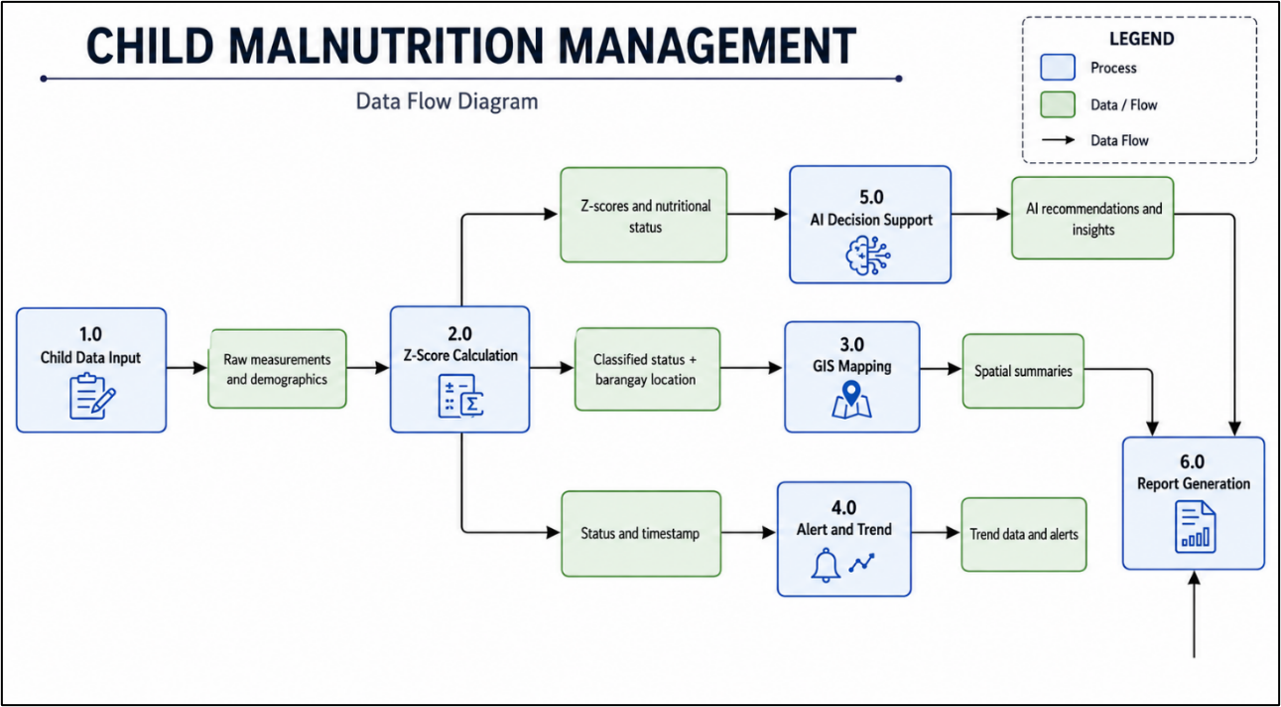
\includegraphics[width=0.95\textwidth]{dfd.png}
    \caption{Data Flow Diagram}
    \label{fig:dfd}
\end{figure}

\noindent \textbf{\textit{External Entities Interaction}}

\vspace{0.3cm}
\begin{longtable}{p{3.5cm} p{10.5cm}}
    \caption{External Entities Interaction in DFD} \label{tab:dfd_interaction} \\
    \toprule
    \textbf{External Entity} & \textbf{Interaction with System} \\
    \midrule
    \endfirsthead
    \multicolumn{2}{c}{{\tablename\ \thetable{} -- Continued from previous page}} \\
    \toprule
    \textbf{External Entity} & \textbf{Interaction with System} \\
    \midrule
    \endhead
    \midrule
    \multicolumn{2}{r}{{Continued on next page}} \\
    \endfoot
    \bottomrule
    \endlastfoot
    Barangay Health Worker (BHW) & Provides child demographic data and anthropometric measurements \(\rightarrow\) Process 1.0 \\
    \addlinespace
    Barangay Admin & Manages BHW accounts, generates barangay reports, views heatmap and AI recommendations for their barangay \(\leftarrow\) Process 3.0, 5.0, 6.0 \\
    \addlinespace
    Super Admin (CHO) & Manages all user accounts, all barangay GIS data, views city-wide heatmap, generates city-wide reports, configures system settings, receives alerts \(\leftarrow\) Process 3.0, 4.0, 5.0, 6.0 \\
    \addlinespace
    System Administrator & Performs system maintenance, database backup, and views system logs (Backend - No Frontend Access) \\
\end{longtable}
\vspace{0.3cm}

\noindent \textbf{\textit{Data Flow Description}}

The data flow through the system follows this sequence:
\begin{enumerate}
    \item Barangay Health Worker provides child demographic data and anthropometric measurements \(\rightarrow\) Process 1.0 (Child Data Input)
    \item Process 1.0 sends raw measurements and demographics \(\rightarrow\) Process 2.0 (Z-Score and Status Calculation)
    \item Process 2.0 calculates Z-scores and classifies nutritional status
    \item Process 2.0 sends classified status + barangay location \(\rightarrow\) Process 3.0 (GIS Mapping)
    \item Process 2.0 sends status and timestamp \(\rightarrow\) Process 4.0 (Alert and Trend)
    \item Process 2.0 sends Z-scores and nutritional status \(\rightarrow\) Process 5.0 (AI Decision Support)
    \item Process 5.0 generates evidence-based recommendations and prioritizes high-risk cases
    \item Process 5.0 sends AI recommendations and insights \(\rightarrow\) Process 6.0 (Report Generation)
    \item Process 3.0 sends spatial summaries \(\rightarrow\) Process 6.0 (Report Generation)
    \item Process 4.0 sends trend data and alerts \(\rightarrow\) Process 6.0 (Report Generation)
    \item Process 6.0 produces automated reports (PDF and Excel formats) for barangay or city-level summaries
\end{enumerate}

\noindent \textbf{\textit{System Outputs}}

The system produces the following outputs:
\vspace{0.3cm}
\begin{longtable}{p{3cm} p{8cm} p{3cm}}
    \caption{System Outputs} \label{tab:system_outputs} \\
    \toprule
    \textbf{Output Type} & \textbf{Description} & \textbf{Source Process} \\
    \midrule
    \endfirsthead
    \multicolumn{3}{c}{{\tablename\ \thetable{} -- Continued from previous page}} \\
    \toprule
    \textbf{Output Type} & \textbf{Description} & \textbf{Source Process} \\
    \midrule
    \endhead
    \midrule
    \multicolumn{3}{r}{{Continued on next page}} \\
    \endfoot
    \bottomrule
    \endlastfoot
    Interactive Heatmap & Color-coded map showing malnutrition cases by barangay & Process 3.0 GIS Mapping \\
    \addlinespace
    Child Growth Charts & Individual growth curves plotted against WHO standards & Process 2.0 Z-Score Calculation \\
    \addlinespace
    Malnutrition Trend Graphs & Bar charts and line charts showing cases over time & Process 4.0 Alert and Trend \\
    \addlinespace
    Early Warning Alerts & Dashboard notifications for barangays exceeding thresholds & Process 4.0 Alert and Trend \\
    \addlinespace
    AI Recommendations & Evidence-based nutritional intervention suggestions & Process 5.0 AI Decision Support \\
    \addlinespace
    Risk Prioritization & Ranked list of high-risk children and barangays & Process 5.0 AI Decision Support \\
    \addlinespace
    Automated Reports & PDF and Excel reports summarizing malnutrition cases & Process 6.0 Report Generation \\
\end{longtable}
\vspace{0.3cm}

\subsection{UML Use Case Diagram}
\label{subsec:usecase}
The Use Case Diagram illustrates the functional requirements of the Health Monitoring System with GIS and AI Decision Support from the perspective of four user roles: Barangay Health Worker (BHW), Barangay Admin, Super Admin (City Health Office), and System Administrator.

\begin{figure}[H]
    \centering
    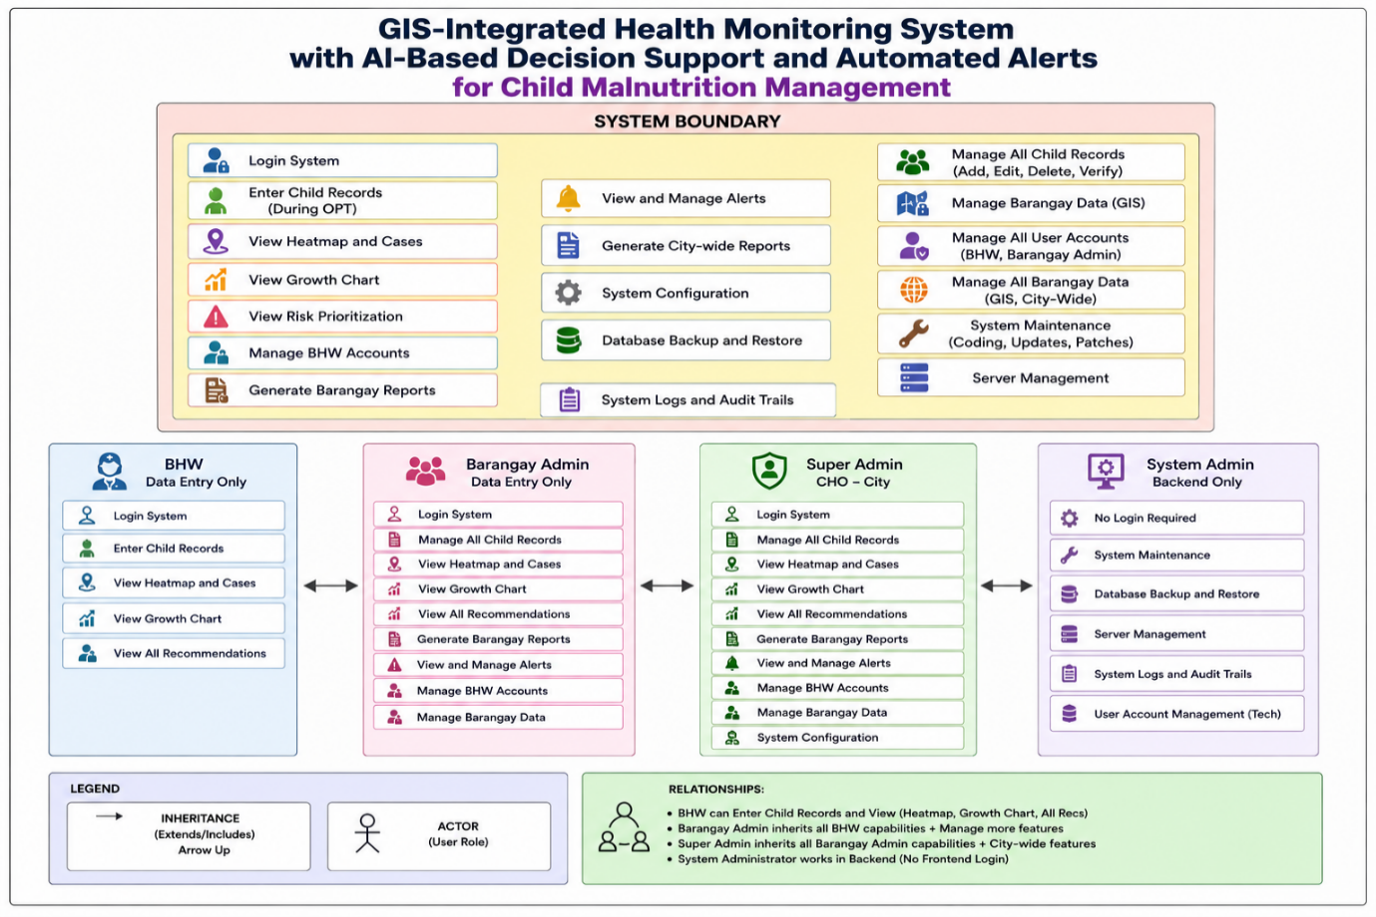
\includegraphics[width=0.95\textwidth]{use_case.png}
    \caption{Use Case Diagram of the GIS-Integrated Health Monitoring System with AI Based Decision Support and Automated Alert for Child Malnutrition Management}
    \label{fig:use_case}
\end{figure}

\noindent \textbf{\textit{Actors and Their Use Cases}}

\vspace{0.3cm}
\begin{longtable}{p{3.5cm} p{5.5cm} p{5.5cm}}
    \caption{Actors and Their Use Cases} \label{tab:actors} \\
    \toprule
    \textbf{Actor} & \textbf{Description} & \textbf{Use Cases} \\
    \midrule
    \endfirsthead
    \multicolumn{3}{c}{{\tablename\ \thetable{} -- Continued from previous page}} \\
    \toprule
    \textbf{Actor} & \textbf{Description} & \textbf{Use Cases} \\
    \midrule
    \endhead
    \midrule
    \multicolumn{3}{r}{{Continued on next page}} \\
    \endfoot
    \bottomrule
    \endlastfoot
    Barangay Health Worker (BHW) & Frontline health worker responsible for data collection and data entry during Operation Timbang (OPT) at the barangay level & • Login System • Enter Child Records (add child data from OPT) • View Growth Chart • View Heatmap and Cases • View AI Recommendations \\
    \addlinespace
    Barangay Admin & Health officer assigned to a specific barangay who manages and oversees BHWs and all barangay-level health data & • Login System • Manage BHW Accounts (create, edit, delete BHWs) • Manage All Child Records (add, edit, delete, verify) • View Growth Chart • View Heatmap and Cases • View AI Recommendations • View Risk Prioritization • Generate Barangay Reports (PDF/XLS) • View and Manage Alerts • Manage Barangay Data (GIS) \\
    \addlinespace
    Super Admin (CHO) & City Health Officer or designated staff at the City Health Office with city-wide oversight & • Login System • Manage All User Accounts (BHW, Barangay Admin) • Manage All Barangay Data (GIS) • View City-wide Heatmap and Cases • View Growth Chart (for analysis) • View AI Recommendations • View Risk Prioritization • Generate City-wide Reports (PDF/XLS) • Receive and Manage Alerts • System Configuration \\
    \addlinespace
    System Administrator & IT personnel responsible for technical system maintenance, server management, and database administration (Backend - No Frontend Login Required) & • System Maintenance (coding, updates, patches) • Database Backup and Restore • Server Management • System Logs and Audit Trails (backend) • User Account Management (technical support) \\
\end{longtable}
\vspace{0.3cm}

\noindent \textbf{\textit{Use Case Descriptions}}

\vspace{0.3cm}
\begin{longtable}{p{3.5cm} p{7cm} p{4cm}}
    \caption{Use Case Descriptions} \label{tab:usecase_desc} \\
    \toprule
    \textbf{Use Case} & \textbf{Description} & \textbf{Users} \\
    \midrule
    \endfirsthead
    \multicolumn{3}{c}{{\tablename\ \thetable{} -- Continued from previous page}} \\
    \toprule
    \textbf{Use Case} & \textbf{Description} & \textbf{Users} \\
    \midrule
    \endhead
    \midrule
    \multicolumn{3}{r}{{Continued on next page}} \\
    \endfoot
    \bottomrule
    \endlastfoot
    Login System & User authentication and access control for frontend users & BHW, Barangay Admin, Super Admin \\
    \addlinespace
    Enter Child Records & Add child data collected during Operation Timbang (OPT) & BHW \\
    \addlinespace
    Manage All Child Records & Add, edit, delete, and verify child nutritional data & Barangay Admin \\
    \addlinespace
    View Heatmap and Cases & Interactive GIS heatmap visualization of malnutrition cases & BHW, Barangay Admin, Super Admin \\
    \addlinespace
    View Growth Chart & Individual child growth monitoring against WHO standards & BHW, Barangay Admin, Super Admin \\
    \addlinespace
    View AI Recommendations & AI-generated nutritional intervention recommendations & BHW, Barangay Admin, Super Admin \\
    \addlinespace
    View Risk Prioritization & Ranked list of high-risk children and barangays & Barangay Admin, Super Admin \\
    \addlinespace
    Generate Barangay Reports & PDF/XLS report generation for a specific barangay & Barangay Admin \\
    \addlinespace
    Generate City-wide Reports & PDF/XLS report generation for the entire city & Super Admin \\
    \addlinespace
    View and Manage Alerts & View, acknowledge, and resolve early warning alerts & Barangay Admin, Super Admin \\
    \addlinespace
    Manage BHW Accounts & Create, edit, and manage BHW accounts for their barangay & Barangay Admin \\
    \addlinespace
    Manage All User Accounts & Create, edit, and manage all user accounts (BHW, Barangay Admin) & Super Admin \\
    \addlinespace
    Manage Barangay Data (GIS) & Manage barangay boundaries and GIS data for their barangay & Barangay Admin \\
    \addlinespace
    Manage All Barangay Data (GIS) & Manage all barangay boundaries and GIS data city-wide & Super Admin \\
    \addlinespace
    System Configuration & Configure system settings, thresholds, and alert parameters & Super Admin \\
    \addlinespace
    System Maintenance & Coding, updates, patches, and technical maintenance & System Administrator (Backend) \\
    \addlinespace
    Database Backup and Restore & Database backup and restore operations & System Administrator (Backend) \\
    \addlinespace
    Server Management & Server configuration and management & System Administrator (Backend) \\
    \addlinespace
    System Logs and Audit Trails & View and monitor system logs and audit trails & System Administrator (Backend) \\
    \addlinespace
    User Account Management (Technical) & Technical support for user accounts & System Administrator (Backend) \\
\end{longtable}
\vspace{0.3cm}

This diagram illustrates the hierarchical relationship among the four user roles of the system.

\begin{figure}[H]
    \centering
    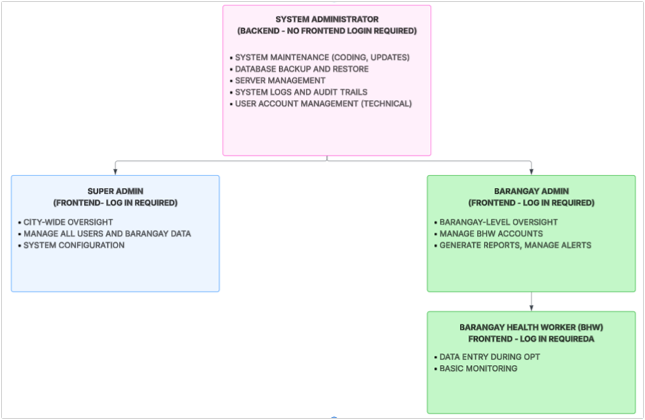
\includegraphics[width=0.95\textwidth]{actor_hierarchy.png}
    \caption{Actor Hierarchy Diagram of the GIS-Integrated Health Monitoring System with AI-Based Decision Support and Automated Alert for Child Malnutrition Management}
    \label{fig:actor_hierarchy}
\end{figure}

\noindent \textbf{\textit{Relationships}}

\vspace{0.3cm}
\begin{longtable}{p{3.5cm} p{10.5cm}}
    \caption{Relationships} \label{tab:relationships} \\
    \toprule
    \textbf{Relationship} & \textbf{Description} \\
    \midrule
    \endfirsthead
    \multicolumn{2}{c}{{\tablename\ \thetable{} -- Continued from previous page}} \\
    \toprule
    \textbf{Relationship} & \textbf{Description} \\
    \midrule
    \endhead
    \midrule
    \multicolumn{2}{r}{{Continued on next page}} \\
    \endfoot
    \bottomrule
    \endlastfoot
    Shared Use Cases & View Heatmap and Cases, View AI Recommendations, and View Growth Chart are shared by BHW, Barangay Admin, and Super Admin \\
    \addlinespace
    BHW Exclusive & Enter Child Records (data entry during Operation Timbang) \\
    \addlinespace
    Barangay Admin Exclusive & Manage BHW Accounts, Manage All Child Records, Generate Barangay Reports, View Risk Prioritization, View and Manage Alerts, Manage Barangay Data (GIS) \\
    \addlinespace
    Super Admin Exclusive & Manage All User Accounts, Manage All Barangay Data, Generate City-wide Reports, System Configuration \\
    \addlinespace
    System Administrator Exclusive (Backend) & System Maintenance, Database Backup, Server Management, System Logs, User Account Management (Technical) \\
    \addlinespace
    Inheritance & Barangay Admin inherits all BHW use cases (can also enter data); Super Admin inherits all Barangay Admin use cases \\
\end{longtable}
\vspace{0.3cm}

\subsection{Entity Relationship Diagram}
\label{subsec:erd}
The database is designed using PostgreSQL with PostGIS spatial extensions.

\noindent \textbf{\textit{Entities and Attributes}}

\begin{itemize}
    \item \textbf{Child entity} has attributes: child\_id as primary key, full\_name, birthdate, sex, address, guardian\_name, contact\_number, barangay\_id as foreign key, purok\_id as foreign key, edema\_status, measurement\_method, and indigenous\_child.
    \item \textbf{Health\_Record entity} has attributes: record\_id as primary key, child\_id as foreign key, weight\_kg, height\_cm, date\_measured, measurement\_method, and user\_id as foreign key.
    \item \textbf{Nutrition\_Status entity} has attributes: status\_id as primary key, record\_id as foreign key, weight\_for\_age\_z, height\_for\_age\_z, weight\_for\_height\_z, classification, map\_color, priority\_level, and remarks.
    \item \textbf{Barangay entity} has attributes: barangay\_id as primary key, barangay\_name, population, boundary stored as a PostGIS POLYGON spatial data type, risk\_level, total\_cases, malnutrition\_threshold, and last\_updated.
    \item \textbf{Purok entity} has attributes: purok\_id as primary key, purok\_name, barangay\_id as foreign key, boundary stored as a PostGIS POLYGON spatial data type, population, and risk\_level.
    \item \textbf{User entity} has attributes: user\_id as primary key, full\_name, role (bhw, barangay\_admin, super\_admin, or system\_admin), username, password\_hash, barangay\_id as foreign key for BHW and Barangay Admin users, and last\_login.
    \item \textbf{Alert entity} has attributes: alert\_id as primary key, barangay\_id as foreign key, purok\_id as foreign key, alert\_level (Warning, Critical, or Emergency), prevalence\_value, threshold\_value, date\_triggered, and status (Active, Acknowledged, or Resolved).
    \item \textbf{Report entity} has attributes: report\_id as primary key, report\_type (Barangay, Purok, or City), barangay\_id as foreign key (NULL if city-wide), purok\_id as foreign key (NULL if barangay/city-wide), date\_from, date\_to, date\_generated, file\_path, and generated\_by as foreign key referencing user\_id.
\end{itemize}

\noindent \textbf{\textit{Relationships}}

The relationships among the entities are as follows:

\begin{itemize}
    \item \textbf{Barangay to Purok.} One Barangay can have many Puroks. This relationship enables the system to organize child nutrition data at the purok level within each barangay, allowing for more granular monitoring and targeted interventions.
    \item \textbf{Barangay to Child.} One Barangay can have many Child records. This relationship links each child to their barangay of residence, enabling barangay-level aggregation and analysis of malnutrition cases.
    \item \textbf{Purok to Child.} One Purok can have many Child records. This relationship links each child to their specific purok or sitio within the barangay, allowing for purok-level visualization and prioritization.
    \item \textbf{Child to Health\_Record.} One Child can have many Health\_Record entries. This one-to-many relationship supports longitudinal growth monitoring, allowing health workers to track changes in a child's weight, height, and nutritional status over time.
    \item \textbf{Health\_Record to Nutrition\_Status.} One Health\_Record has one corresponding Nutrition\_Status record. This one-to-one relationship stores the calculated Z-scores and nutritional status classification derived from each health record.
    \item \textbf{User to Health\_Record.} One User can record many Health\_Record entries. This relationship tracks which health worker or nutrition officer recorded each child's measurements, ensuring accountability and auditability.
    \item \textbf{User to Report.} One User can generate many Reports. This relationship tracks who generated each report, enabling audit trails for reporting activities.
    \item \textbf{Barangay to Alert.} One Barangay can generate many Alert records. This relationship enables the system to track multiple alerts for a barangay over time, including historical alert data for trend analysis.
    \item \textbf{Purok to Alert.} One Purok can generate many Alert records. This relationship enables the system to generate and track alerts at the purok level, allowing for more targeted notifications and interventions.
    \item \textbf{Barangay to Report.} One Barangay can have many Report records. This relationship enables the generation of barangay-specific reports for nutrition monitoring and program evaluation.
    \item \textbf{Purok to Report.} One Purok can have many Report records. This relationship enables the generation of purok-specific reports for localized nutrition monitoring.
\end{itemize}

The PostGIS spatial implementation requires that the Barangay and Purok boundary columns store polygon shapes using PostGIS's POINT and POLYGON data types. This enables spatial queries such as finding all children within a given barangay or purok boundary using functions like ST\_Contains() and ST\_Intersects(). These spatial functions are critical for the system's heatmap visualization and risk level analysis features.

\begin{figure}[H]
    \centering
    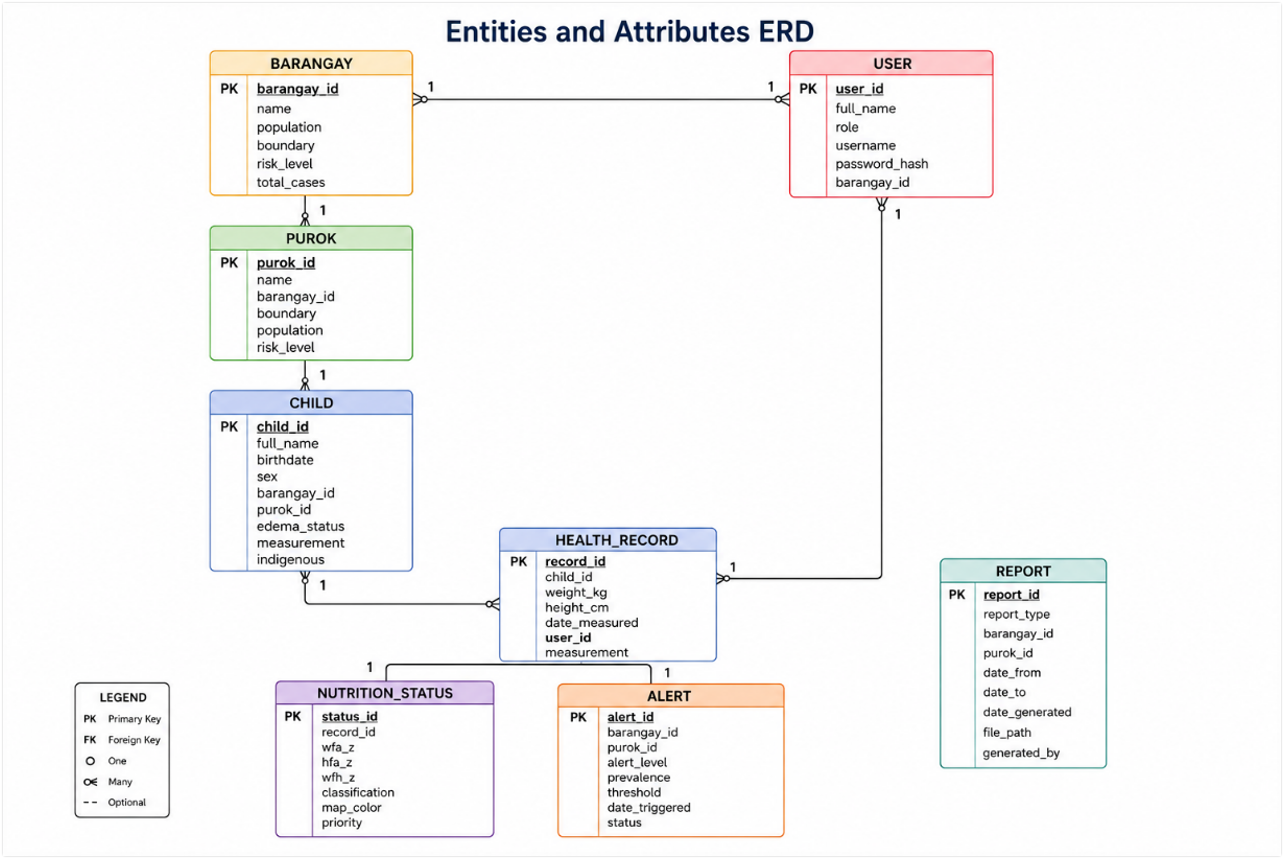
\includegraphics[width=0.95\textwidth]{erd.png}
    \caption{Entity Relationship Diagram (ERD) of the GIS-Integrated Health Monitoring System with AI Based Decision Support and Automated Alert for Child Malnutrition Management}
    \label{fig:erd}
\end{figure}

\subsection{System Architecture}
\label{subsec:architecture}
The proposed system follows a layered architecture: presentation tier (frontend), application tier (backend server), data tier (database), and GIS engine.

\noindent \textbf{\textit{Users}}

The system accommodates four types of users:

\vspace{0.3cm}
\begin{longtable}{p{3cm} p{6cm} p{5cm}}
    \caption{System Users} \label{tab:users} \\
    \toprule
    \textbf{User Type} & \textbf{Description} & \textbf{Access Level} \\
    \midrule
    \endfirsthead
    \multicolumn{3}{c}{{\tablename\ \thetable{} -- Continued from previous page}} \\
    \toprule
    \textbf{User Type} & \textbf{Description} & \textbf{Access Level} \\
    \midrule
    \endhead
    \midrule
    \multicolumn{3}{r}{{Continued on next page}} \\
    \endfoot
    \bottomrule
    \endlastfoot
    Barangay Health Worker (BHW) & Frontline health worker responsible for data entry and basic monitoring at the barangay level & Barangay-level data only \\
    \addlinespace
    Barangay Admin & Health officer assigned to a specific barangay who oversees BHWs and manages barangay-level data & Barangay-level data + BHW management \\
    \addlinespace
    Super Admin (CHO) & City Health Officer or designated staff at the City Health Office with city-wide oversight & City-wide data + user management + system configuration \\
    \addlinespace
    System Administrator & IT personnel responsible for technical system maintenance & System-level access (maintenance, backup, logs) \\
\end{longtable}
\vspace{0.3cm}

\noindent \textbf{\textit{Presentation Tier (Frontend)}}

The frontend is built using the Next.js framework with HTML5, CSS3, and JavaScript. It consists of four main components: Dashboard for displaying key metrics, Map Viewer (GIS) for interactive mapping powered by Leaflet.js, Data Entry Forms for recording child anthropometric measurements, and Reports \& Charts for visualizing malnutrition trends.

\noindent \textbf{\textit{Application Tier (Backend Server)}}

The backend is developed in Python using the FastAPI framework. FastAPI is chosen for its high performance, automatic API documentation, and asynchronous request handling. The backend is organized into seven modules:

\begin{enumerate}
    \item Authentication Module -- Handles user login, session management, and password hashing
    \item Child Management Module -- Manages CRUD operations for child records
    \item Health Record Processing -- Processes weight, height, and age data
    \item Nutrition Status Analyzer -- Implements OPT Plus algorithm pipeline with Z-score calculation, edema override, and classification based on the NNC OPT Plus Guidelines [50]
    \item Alert System -- Monitors malnutrition trends and generates 3-tier alerts (Warning, Critical, Emergency)
    \item AI Decision Support Module -- Automatically analyzes Z-scores, prevalence data, and growth trends to identify barangays with elevated malnutrition risk and recommend appropriate interventions using rule-based classification and prevalence analysis based on NNC OPT Plus Guidelines
    \item Report Generator -- Produces PDF and Excel reports with AI insights
\end{enumerate}

\noindent \textbf{\textit{AI Decision Support Module Details}}

\vspace{0.3cm}
\begin{longtable}{p{3.5cm} p{10.5cm}}
    \caption{AI Decision Support Module Details} \label{tab:ai_modules} \\
    \toprule
    \textbf{Sub-Module} & \textbf{Description} \\
    \midrule
    \endfirsthead
    \multicolumn{2}{c}{{\tablename\ \thetable{} -- Continued from previous page}} \\
    \toprule
    \textbf{Sub-Module} & \textbf{Description} \\
    \midrule
    \endhead
    \midrule
    \multicolumn{2}{r}{{Continued on next page}} \\
    \endfoot
    \bottomrule
    \endlastfoot
    Recommendation Engine & Generates automatic nutritional intervention suggestions based on barangay/purok prevalence data and OPT Plus standards [50]. \\
    \addlinespace
    Rule-Based Classification Engine & Applies OPT Plus classification standards to analyze Z-scores and prevalence data [50]. \\
    \addlinespace
    Risk Prioritization & Ranks children, puroks, and barangays by severity of malnutrition, enabling health workers to focus on the most critical cases first. \\
    \addlinespace
    Intelligent Insights & Identifies patterns and trends in malnutrition data, suggesting potential intervention strategies. \\
\end{longtable}
\vspace{0.3cm}

\noindent \textbf{\textit{Data Tier (Database)}}

The database is implemented using PostgreSQL with the PostGIS extension to support both relational data management and advanced geospatial queries. PostGIS provides comprehensive spatial data types (POINT, POLYGON, MULTIPOLYGON) and robust functions such as ST\_Contains() and ST\_Distance() for efficient barangay boundary storage and child record geolocation. To achieve real-time monitoring and alert generation, the system employs a polling-based mechanism combined with PostgreSQL triggers and backend event handling. Specifically:

\begin{itemize}
    \item A lightweight AJAX polling mechanism (every 5 seconds) from the Next.js frontend to the Python backend checks for new alerts, recently updated child records, and threshold breaches.
    \item PostgreSQL AFTER INSERT and AFTER UPDATE triggers log changes to a realtime\_events table, which the backend queries to push near-real-time updates to the dashboard.
    \item For critical alerts (e.g., severe wasting prevalence \(\geq 5\%\)), the backend immediately updates the dashboard via WebSocket connections (using FastAPI's WebSocket support or Socket.IO) to notify city health officers without requiring a page refresh.
\end{itemize}

The database stores data across five main tables: child, user, health\_record, barangay, and alert. PostgreSQL spatial indexes using GiST (Generalized Search Tree) structures ensure fast geospatial queries, enabling real-time heatmap rendering and risk level analysis as soon as new anthropometric data is entered. Additionally, the geography data type available in PostGIS allows for precise meter-based proximity searches between child locations and barangay boundaries---a critical feature for accurate public health monitoring within the City Health Office.

\noindent \textbf{\textit{GIS Engine and Map Service}}

The GIS component is implemented using Leaflet.js for frontend mapping, integrated with PostGIS (within Supabase/PostgreSQL) for backend spatial queries and data storage. The GIS Engine handles three key functions:

\begin{itemize}
    \item \textbf{Heatmap Visualization} -- Displays malnutrition density across Cabadbaran City using color-coded overlays. The backend executes PostGIS spatial queries (e.g., ST\_Contains(), ST\_Intersects()) to aggregate child records by barangay polygons, then returns GeoJSON data to Leaflet.js for rendering.
    \item \textbf{Barangay Mapping} -- Displays barangay boundaries stored as POLYGON or MULTIPOLYGON geometries in PostgreSQL using PostGIS. Click-for-details functionality is implemented by sending the clicked barangay ID to the backend, which runs a spatial query to retrieve malnutrition statistics (e.g., count of severe cases, prevalence rate) from the child and health\_record tables joined with the barangay table.
    \item \textbf{Risk Level Analysis} -- Classifies each barangay as Low Risk, Moderate Risk, or Severe Risk based on malnutrition prevalence thresholds. The classification logic is implemented either as a PostgreSQL stored function (PL/pgSQL) or computed in the Python backend after retrieving aggregated data via spatial queries.
\end{itemize}

\noindent \textbf{\textit{Technology Stack for GIS:}}

\begin{itemize}
    \item Frontend mapping: Leaflet.js with OpenStreetMap tiles
    \item Spatial data storage: PostGIS geometry and geography data types (POINT, POLYGON, MULTIPOLYGON)
    \item Spatial indexing: PostgreSQL GiST (Generalized Search Tree) indexes for fast spatial queries and nearest-neighbor searches
    \item Spatial functions: ST\_Contains(), ST\_Within(), ST\_Intersects(), ST\_Distance() (with geography casting for precise meter-based calculations)
\end{itemize}

\noindent \textbf{\textit{Output System.}} The system produces three types of outputs:

\begin{itemize}
    \item \textbf{Reports} -- PDF and Excel reports generated by the Report Generator module, downloadable by users
    \item \textbf{Alerts} -- Automatically triggered notifications (Warning - Yellow, Critical - Orange, Emergency - Red) displayed on the dashboard when malnutrition thresholds are exceeded
    \item \textbf{AI Recommendations} -- Evidence-based nutritional intervention suggestions displayed on the dashboard and included in reports
\end{itemize}

\begin{figure}[H]
    \centering
    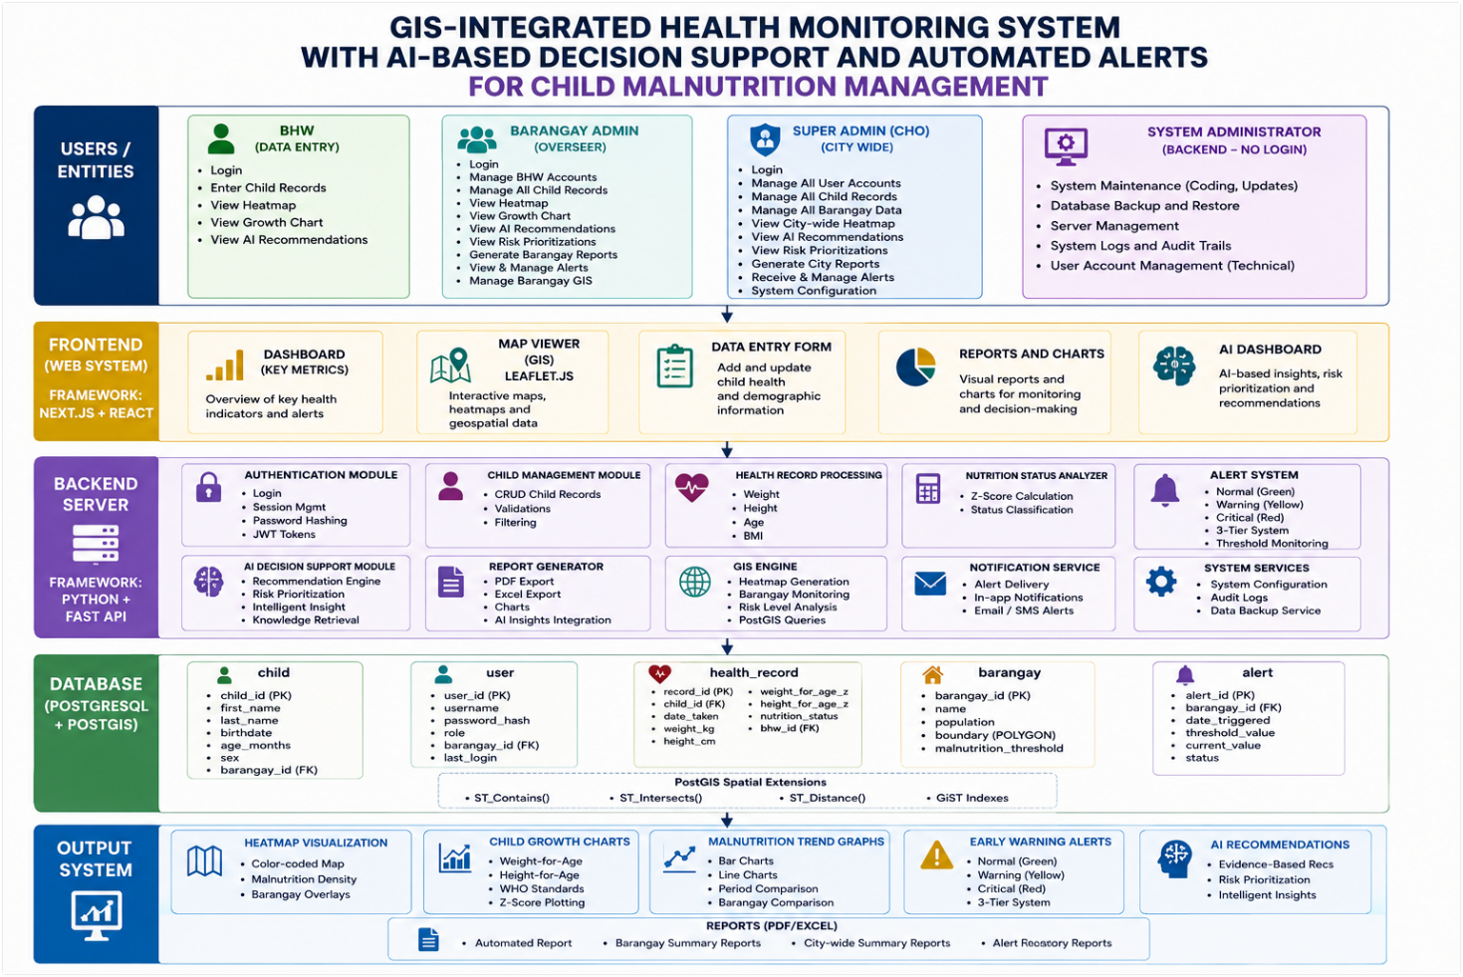
\includegraphics[width=0.95\textwidth]{system_architecture.png}
    \caption{System Architecture, GIS-Integrated Health Monitoring System with AI Based Decision Support and Automated Alert for Child Malnutrition Management}
    \label{fig:system_arch}
\end{figure}

\subsection{Algorithm Design}
\label{subsec:algorithm}
The system implements the following algorithms to ensure accurate nutritional status classification and alert generation based on NNC OPT Plus guidelines [49] and WHO standards.

\noindent \textbf{\textit{Algorithm 1: Age Calculation (Chronological Milestone Resolution)}}

The system calculates a child's age by finding the exact interval between the date of birth and the measurement date. Per NNC OPT Plus guidelines [50], any remaining days are disregarded and not considered in the computation of age in months.

NNC Age Computation Rule [50]: ``To compute the age in months, compute the child's age to the nearest month as of her birth date. For example, a child born on 01 October 2004 and measured on 21 August 2007 is 2 years, 10 months and 20 days. Disregarding the number of days, the child is 34 months old (2 years multiplied by 12, plus 10 months equals 34 months).''

\begin{equation}
    \text{Age (in months)} = \text{FLOOR}\left(\frac{\text{Measurement Date} - \text{Birth Date}}{30.4375}\right)
\end{equation}

Example: An infant aged 6 months and 28 days is mapped directly onto the Month 6 reference parameters.

\noindent \textbf{\textit{Algorithm 2: Height/Length Positional Adjustment}}

Human growth standards differentiate between recumbent length (lying down) and standing height. The system evaluates the entry using a conditional switch as specified in the NNC OPT Plus Guidelines [50]:

\vspace{0.3cm}
\begin{longtable}{p{3cm} p{5cm} p{5cm}}
    \caption{Height/Length Positional Adjustment} \label{tab:positional_adj} \\
    \toprule
    \textbf{Age Group} & \textbf{Measurement Method} & \textbf{Adjustment} \\
    \midrule
    \endfirsthead
    \multicolumn{3}{c}{{\tablename\ \thetable{} -- Continued from previous page}} \\
    \toprule
    \textbf{Age Group} & \textbf{Measurement Method} & \textbf{Adjustment} \\
    \midrule
    \endhead
    \midrule
    \multicolumn{3}{r}{{Continued on next page}} \\
    \endfoot
    \bottomrule
    \endlastfoot
    0-23 months & Standing (incorrect) & Add +0.7 cm \\
    \addlinespace
    0-23 months & Lying down (correct) & No adjustment \\
    \addlinespace
    24-71 months & Lying down (incorrect) & Subtract -0.7 cm \\
    \addlinespace
    24-71 months & Standing (correct) & No adjustment \\
\end{longtable}
\vspace{0.3cm}

NNC Measurement Protocol [49]:
\begin{itemize}
    \item ``If the child is 0-23 months old, measure the child's length lying down (recumbent). If the child is 24-71 months old, measure the child's standing height.''
    \item ``If the child is 0-23 months old will not be taken for measurement of length, the standing height may be measured. Just add 0.7 cm to convert to length from the child's height.''
    \item ``If the child is 24-71 months old who will not stand up may be measured lying down. Just subtract 0.7 cm.''
\end{itemize}

Rounding Rule [49]: Upon taking the child's height/length, round off the actual reading to the nearest 0.5 cm:
\begin{itemize}
    \item Example: 51.3 cm \(\rightarrow\) refer to 51.5 cm
    \item Example: 56.3 cm \(\rightarrow\) refer to 56.5 cm
\end{itemize}

\noindent \textbf{Algorithmic Logic:}
\begin{verbatim}
Height = ROUND(Height * 2) / 2  (Round to nearest 0.5 cm)
IF Age < 24 AND Method == "Standing" THEN
    Height = Height + 0.7
ELSE IF Age >= 24 AND Method == "Lying Down" THEN
    Height = Height - 0.7
ELSE
    Height = Height  (No adjustment)
END IF
\end{verbatim}

\noindent \textbf{\textit{Algorithm 3: Z-Score Calculation (Box-Cox Cole and Green Method)}}

The system uses the WHO Box-Cox Cole and Green (LMS) method to calculate Z-scores, as referenced in the NNC OPT Plus Guidelines [49].

\noindent \textbf{Z-Score Formula:}
\begin{align}
    \text{For } L \neq 0: \quad Z &= \frac{\left(\frac{X}{M}\right)^L - 1}{L \times S} \\
    \text{For } L = 0: \quad Z &= \frac{\ln\left(\frac{X}{M}\right)}{S}
\end{align}

\noindent \textbf{Gender-Specific Parameters:}

\vspace{0.3cm}
\begin{longtable}{p{3.5cm} p{2.5cm} p{3cm} p{3.5cm} p{3cm}}
    \caption{Gender-Specific Parameters (WAZ)} \label{tab:waz_params} \\
    \toprule
    \textbf{Milestone} & \textbf{Sex} & \textbf{L (Skewness)} & \textbf{M (Median Weight)} & \textbf{S (Variation)} \\
    \midrule
    \endfirsthead
    \multicolumn{5}{c}{{\tablename\ \thetable{} -- Continued from previous page}} \\
    \toprule
    \textbf{Milestone} & \textbf{Sex} & \textbf{L (Skewness)} & \textbf{M (Median Weight)} & \textbf{S (Variation)} \\
    \midrule
    \endhead
    \midrule
    \multicolumn{5}{r}{{Continued on next page}} \\
    \endfoot
    \bottomrule
    \endlastfoot
    Month 12 (1 Year) & Boys & -0.3521 & 9.6 kg & 0.1213 \\
    \addlinespace
    Month 12 (1 Year) & Girls & -0.3809 & 8.9 kg & 0.1281 \\
    \addlinespace
    Month 24 (2 Years) & Boys & -0.3521 & 12.2 kg & 0.1173 \\
    \addlinespace
    Month 24 (2 Years) & Girls & -0.3809 & 11.5 kg & 0.1245 \\
\end{longtable}
\vspace{0.3cm}

\noindent \textbf{Height-for-Age Parameters (L = 1.0 for both sexes):}

\vspace{0.3cm}
\begin{longtable}{p{3.5cm} p{2.5cm} p{3cm} p{3.5cm} p{3cm}}
    \caption{Height-for-Age Parameters (HAZ)} \label{tab:haz_params} \\
    \toprule
    \textbf{Milestone} & \textbf{Sex} & \textbf{L (Skewness)} & \textbf{M (Median Height)} & \textbf{S (Variation)} \\
    \midrule
    \endfirsthead
    \multicolumn{5}{c}{{\tablename\ \thetable{} -- Continued from previous page}} \\
    \toprule
    \textbf{Milestone} & \textbf{Sex} & \textbf{L (Skewness)} & \textbf{M (Median Height)} & \textbf{S (Variation)} \\
    \midrule
    \endhead
    \midrule
    \multicolumn{5}{r}{{Continued on next page}} \\
    \endfoot
    \bottomrule
    \endlastfoot
    Month 12 (1 Year) & Boys & 1.0000 & 75.7 cm & 0.0354 \\
    \addlinespace
    Month 12 (1 Year) & Girls & 1.0000 & 74.0 cm & 0.0371 \\
    \addlinespace
    Month 24 (2 Years) & Boys & 1.0000 & 87.8 cm & 0.0364 \\
    \addlinespace
    Month 24 (2 Years) & Girls & 1.0000 & 86.4 cm & 0.0382 \\
\end{longtable}
\vspace{0.3cm}

\noindent \textbf{\textit{Algorithm 4: Clinical Priority Interception (Edema Override)}}

The system integrates a triage override step. If a user flags the presence of bilateral edema during data entry, the mathematical Z-score loops are skipped as specified in the NNC OPT Plus Guidelines [50].

\noindent \textbf{Algorithmic Logic:}
\begin{verbatim}
IF Bilateral_Edema == True THEN
    SKIP Z-score calculations (WAZ, HAZ, WHZ)
    SET Nutritional_Status = "Severe Acute Malnutrition (SAM)"
    SET Priority_Level = "Immediate Emergency"
    TRIGGER Emergency Alert (Red)
    MAP Color = Solid Red
END IF
\end{verbatim}

Rationale: Fluid accumulation artificially alters a child's weight record, making WAZ and WHZ calculations medically invalid [50].

\noindent \textbf{\textit{Algorithm 5: Nutritional Status Classification (OPT Plus Standards)}}

The system classifies each child's nutritional status based on Z-scores and NNC OPT Plus cut-offs [50], enforcing overlapping edge logic (exactly -2.00 is Normal).

\noindent \textbf{Weight-for-Age (WAZ):}

\vspace{0.3cm}
\begin{longtable}{p{3cm} p{3cm} p{3cm} p{3cm}}
    \caption{Weight-for-Age (WAZ) Classification} \label{tab:waz_class} \\
    \toprule
    \textbf{Z-Score Range} & \textbf{OPT Plus Status} & \textbf{Map Color} & \textbf{Priority Level} \\
    \midrule
    \endfirsthead
    \multicolumn{4}{c}{{\tablename\ \thetable{} -- Continued from previous page}} \\
    \toprule
    \textbf{Z-Score Range} & \textbf{OPT Plus Status} & \textbf{Map Color} & \textbf{Priority Level} \\
    \midrule
    \endhead
    \midrule
    \multicolumn{4}{r}{{Continued on next page}} \\
    \endfoot
    \bottomrule
    \endlastfoot
    Z > +2.00 & Overweight & Purple/Blue & Low \\
    \addlinespace
    -2.00 \(\leq\) Z \(\leq\) +2.00 & Normal & Green & Baseline \\
    \addlinespace
    -3.00 \(\leq\) Z < -2.00 & Underweight & Orange & Moderate \\
    \addlinespace
    Z < -3.00 & Severely Underweight & Red & High \\
\end{longtable}
\vspace{0.3cm}

\noindent \textbf{Height-for-Age (HAZ):}

\vspace{0.3cm}
\begin{longtable}{p{3cm} p{3cm} p{3cm} p{3cm}}
    \caption{Height-for-Age (HAZ) Classification} \label{tab:haz_class} \\
    \toprule
    \textbf{Z-Score Range} & \textbf{OPT Plus Status} & \textbf{Map Color} & \textbf{Priority Level} \\
    \midrule
    \endfirsthead
    \multicolumn{4}{c}{{\tablename\ \thetable{} -- Continued from previous page}} \\
    \toprule
    \textbf{Z-Score Range} & \textbf{OPT Plus Status} & \textbf{Map Color} & \textbf{Priority Level} \\
    \midrule
    \endhead
    \midrule
    \multicolumn{4}{r}{{Continued on next page}} \\
    \endfoot
    \bottomrule
    \endlastfoot
    Z > +2.00 & Tall & Purple/Blue & Low \\
    \addlinespace
    -2.00 \(\leq\) Z \(\leq\) +2.00 & Normal & Green & Baseline \\
    \addlinespace
    -3.00 \(\leq\) Z < -2.00 & Stunted & Orange & Moderate \\
    \addlinespace
    Z < -3.00 & Severely Stunted & Red & Critical Chronic \\
\end{longtable}
\vspace{0.3cm}

\noindent \textbf{Weight-for-Height/Length (WHZ):}

\vspace{0.3cm}
\begin{longtable}{p{3cm} p{3cm} p{3cm} p{3cm}}
    \caption{Weight-for-Height/Length (WHZ) Classification} \label{tab:whz_class} \\
    \toprule
    \textbf{Z-Score Range} & \textbf{OPT Plus Status} & \textbf{Map Color} & \textbf{Priority Level} \\
    \midrule
    \endfirsthead
    \multicolumn{4}{c}{{\tablename\ \thetable{} -- Continued from previous page}} \\
    \toprule
    \textbf{Z-Score Range} & \textbf{OPT Plus Status} & \textbf{Map Color} & \textbf{Priority Level} \\
    \midrule
    \endhead
    \midrule
    \multicolumn{4}{r}{{Continued on next page}} \\
    \endfoot
    \bottomrule
    \endlastfoot
    Z > +3.00 & Obese & Purple/Blue & High \\
    \addlinespace
    +2.00 < Z \(\leq\) +3.00 & Overweight & Blue & Moderate \\
    \addlinespace
    -2.00 \(\leq\) Z \(\leq\) +2.00 & Normal & Green & Baseline \\
    \addlinespace
    -3.00 \(\leq\) Z < -2.00 & Wasted (Thin) & Orange & High Acute \\
    \addlinespace
    Z < -3.00 & Severely Wasted & Red & Emergency Immediate \\
\end{longtable}
\vspace{0.3cm}

\noindent \textbf{\textit{Algorithm 6: 3-Tier Alert Generation}}

The system employs a 3-tier early warning alert system based on NNC OPT Plus guidelines [49] and WHO thresholds.

\vspace{0.3cm}
\begin{longtable}{p{2.5cm} p{2cm} p{4.5cm} p{4.5cm}}
    \caption{3-Tier Alert Generation} \label{tab:alert_generation} \\
    \toprule
    \textbf{Alert Level} & \textbf{Color} & \textbf{Condition} & \textbf{Action Required} \\
    \midrule
    \endfirsthead
    \multicolumn{4}{c}{{\tablename\ \thetable{} -- Continued from previous page}} \\
    \toprule
    \textbf{Alert Level} & \textbf{Color} & \textbf{Condition} & \textbf{Action Required} \\
    \midrule
    \endhead
    \midrule
    \multicolumn{4}{r}{{Continued on next page}} \\
    \endfoot
    \bottomrule
    \endlastfoot
    Warning & Yellow & Total malnutrition prevalence \(\geq 10\%\) & \begin{tabular}[c]{@{}p{4.2cm}@{}}• Notify Barangay Health Worker\\ • Schedule follow-up assessment\end{tabular} \\
    \addlinespace
    Critical & Orange & Wasting \(\geq 5\%\) OR Any Indicator \(\geq 15\%\) & \begin{tabular}[c]{@{}p{4.2cm}@{}}• Notify Barangay Admin\\ • Conduct supplementary feeding\end{tabular} \\
    \addlinespace
    Emergency & Red & Wasting \(\geq 10\%\) OR SAM \(\geq 2\%\) & \begin{tabular}[c]{@{}p{4.2cm}@{}}• Notify City Health Office\\ • Immediate intervention\end{tabular} \\
\end{longtable}
\vspace{0.3cm}

\noindent \textbf{Alert Triggering Logic:}
\begin{verbatim}
IF Prevalence >= 10% AND < 15% THEN
    TRIGGER Warning Alert (Yellow)
ELSE IF Wasting >= 5% OR Any Indicator >= 15% OR >= 25% increase THEN
    TRIGGER Critical Alert (Orange)
ELSE IF Wasting >= 10% OR SAM >= 2% OR Any Indicator >= 20% THEN
    TRIGGER Emergency Alert (Red)
END IF
\end{verbatim}

\noindent \textbf{\textit{Algorithm 7: AI-Based Decision Support (Rule-Based Classification and Prevalence Analysis)}}

The system automatically analyzes input data and generates intelligent recommendations for child nutrition interventions using rule-based classification and prevalence analysis [9][10][50].

\noindent \textbf{Step 1: Data Analysis}
\begin{itemize}
    \item Automatically analyzes child records, Z-scores, and nutritional status from entered data.
\end{itemize}

\noindent \textbf{Step 2: Prevalence Calculation}
\begin{itemize}
    \item Computes malnutrition prevalence for each barangay and purok based on OPT Plus standards [50].
\end{itemize}

\noindent \textbf{Step 3: Risk Identification}
\begin{itemize}
    \item Identifies barangays and puroks with high cases of wasting, stunting, underweight, or SAM.
\end{itemize}

\noindent \textbf{Step 4: Automatic Decision Support}
\begin{itemize}
    \item Generates automatic recommendations based on prevalence thresholds:
    \begin{itemize}
        \item Warning (Yellow): Prevalence \(\geq 10\%\) \(\rightarrow\) Schedule follow-up assessment.
        \item Critical (Orange): Wasting \(\geq 5\%\) OR Any Indicator \(\geq 15\%\) \(\rightarrow\) Conduct supplementary feeding.
        \item Emergency (Red): Wasting \(\geq 10\%\) OR SAM \(\geq 2\%\) \(\rightarrow\) Immediate intervention required.
    \end{itemize}
\end{itemize}

\noindent \textbf{Step 5: Recommendation Output}
\begin{itemize}
    \item Displays automatic recommendations on the dashboard:
    \begin{itemize}
        \item ``Barangay X is in need of supplementary feeding program''.
        \item ``Purok Y has high wasting cases -- prioritize intervention''.
        \item ``Schedule immediate nutrition assessment for Barangay Z''.
    \end{itemize}
\end{itemize}

\noindent \textbf{Step 6: Human Oversight}
\begin{itemize}
    \item All automatic recommendations require human confirmation before action.
\end{itemize}

\section{Output and User Interface Design}
\label{sec:ui_design}

% [DINI NIMO IBUTANG ANG MGA SCREENSHOTS SA IMONG SYSTEM]
% Pananglitan:
% \begin{figure}[H]
%     \centering
%     \includegraphics[width=0.9\textwidth]{ui_dashboard.png}
%     \caption{System Dashboard}
%     \label{fig:ui_dashboard}
% \end{figure}

\section{Testing Plan}
\label{sec:testing_plan}
This section presents the results of the testing procedures conducted to evaluate the functionality, accuracy, and usability of the developed system. The testing was conducted at three levels: unit testing, integration testing, and user acceptance testing (UAT). The results demonstrate the system's compliance with the identified functional and non-functional requirements, as well as its readiness for deployment within the City Health Office.

Testing is performed at three levels:

\noindent \textbf{Unit Testing.} Each function is tested in isolation using Python's unit test framework (for backend) and Jest (for Next.js frontend). The nutritional status calculator is tested by providing sample measurements and verifying expected classifications. The alert trigger is tested by simulating threshold exceedance.

\noindent \textbf{Integration Testing.} Interactions between modules are tested. Scenarios include: health worker adding child record \(\rightarrow\) verifying data appears on map; generating PDF report \(\rightarrow\) verifying report contains correct records.

\noindent \textbf{User Acceptance Testing (UAT).} Five barangay health workers and the City Program Nutrition Officer will use the system for one week. They will complete an ISO 25010-based questionnaire evaluating functionality, usability, performance, and reliability on a 5-point scale. Acceptance criterion: average score of 4.0 (Agree/Good) or higher.

\subsection{TAM-Based User Acceptance Questionnaire}
\label{subsec:tam_uat}
In addition to the ISO 25010 evaluation, a TAM-based questionnaire will be administered to measure users' perceptions of the system. The questionnaire items are adapted from validated TAM instruments and measure the following constructs:

\vspace{0.3cm}
\begin{longtable}{p{3.5cm} p{10.5cm}}
    \caption{TAM-Based User Acceptance Questionnaire} \label{tab:tam_uat} \\
    \toprule
    \textbf{Construct} & \textbf{Sample Questionnaire Items} \\
    \midrule
    \endfirsthead
    \multicolumn{2}{c}{{\tablename\ \thetable{} -- Continued from previous page}} \\
    \toprule
    \textbf{Construct} & \textbf{Sample Questionnaire Items} \\
    \midrule
    \endhead
    \midrule
    \multicolumn{2}{r}{{Continued on next page}} \\
    \endfoot
    \bottomrule
    \endlastfoot
    Perceived Usefulness (PU) & \begin{tabular}[c]{@{}p{10.5cm}@{}}1. Using the GIS-based health monitoring system would improve my ability to monitor malnutrition cases. \\ 2. The system would help me generate reports more quickly than manual methods. \\ 3. The system would enhance my effectiveness in identifying high-risk barangays. \\ 4. The system would make it easier to track changes in children's nutritional status over time.\end{tabular} \\
    \addlinespace
    Perceived Ease of Use (PEOU) & \begin{tabular}[c]{@{}p{10.5cm}@{}}1. Learning to use the heatmap visualization feature would be easy for me. \\ 2. I would find the system's data entry forms clear and understandable. \\ 3. The system's interface would be intuitive and user-friendly. \\ 4. I would be able to generate reports without assistance.\end{tabular} \\
    \addlinespace
    Facilitating Conditions & \begin{tabular}[c]{@{}p{10.5cm}@{}}1. I have access to the necessary computer equipment to use the system. \\ 2. I have access to reliable internet connectivity for the system. \\ 3. Adequate training will be provided for system use. \\ 4. Technical support will be available when I need it.\end{tabular} \\
    \addlinespace
    Self-Efficacy & \begin{tabular}[c]{@{}p{10.5cm}@{}}1. I am confident in my ability to use the GIS-based system. \\ 2. I can navigate the system even if I have never used a similar system before. \\ 3. I can use the system with the help of the user manual. \\ 4. I can use the system even if there is no one to show me how.\end{tabular} \\
    \addlinespace
    System Quality & \begin{tabular}[c]{@{}p{10.5cm}@{}}1. The system loads quickly and responds promptly. \\ 2. The system accurately calculates Z-scores and nutritional status. \\ 3. The heatmap accurately represents malnutrition cases in each barangay. \\ 4. The system generates reliable and error-free reports.\end{tabular} \\
    \addlinespace
    Perceived Reliability of AI Recommendations & \begin{tabular}[c]{@{}p{10.5cm}@{}}1. I trust the AI-generated recommendations for nutritional interventions. \\ 2. The AI recommendations are based on reliable sources (WHO guidelines). \\ 3. The AI recommendations help me make better decisions. \\ 4. I find the AI recommendations clinically useful.\end{tabular} \\
    \addlinespace
    Perceived Usefulness of AI Features & \begin{tabular}[c]{@{}p{10.5cm}@{}}1. AI recommendations improve my ability to prioritize high-risk children. \\ 2. AI insights help me identify malnutrition patterns quickly. \\ 3. AI recommendations save me time in decision-making. \\ 4. The risk prioritization feature is valuable for my work.\end{tabular} \\
    \addlinespace
    Behavioral Intention (BI) & \begin{tabular}[c]{@{}p{10.5cm}@{}}1. I intend to use the system regularly for monitoring child malnutrition. \\ 2. I will recommend the system to other health workers. \\ 3. I plan to use the system for all my nutrition monitoring tasks. \\ 4. I will continue using the system even if it is not mandatory.\end{tabular} \\
    \addlinespace
    Actual System Use (AU) & \begin{tabular}[c]{@{}p{10.5cm}@{}}1. I use the system frequently for data entry and monitoring. \\ 2. I rely on the system for generating reports. \\ 3. I use the system to identify high-risk barangays. \\ 4. I check the system for early warning alerts regularly.\end{tabular} \\
\end{longtable}
\vspace{0.3cm}

Each item will be rated on a 5-point Likert scale:

\vspace{0.3cm}
\begin{longtable}{p{2cm} p{4cm} p{5cm}}
    \caption{Likert Scale for Questionnaire} \label{tab:likert_quest} \\
    \toprule
    \textbf{Scale} & \textbf{Rating} & \textbf{Interpretation} \\
    \midrule
    \endfirsthead
    \multicolumn{3}{c}{{\tablename\ \thetable{} -- Continued from previous page}} \\
    \toprule
    \textbf{Scale} & \textbf{Rating} & \textbf{Interpretation} \\
    \midrule
    \endhead
    \midrule
    \multicolumn{3}{r}{{Continued on next page}} \\
    \endfoot
    \bottomrule
    \endlastfoot
    5 & Strongly Agree & Excellent \\
    \addlinespace
    4 & Agree & Good \\
    \addlinespace
    3 & Neutral & Fair \\
    \addlinespace
    2 & Disagree & Poor \\
    \addlinespace
    1 & Strongly Disagree & Very Poor \\
\end{longtable}
\vspace{0.3cm}

\section{Deployment Plan}
\label{sec:deployment}
This section outlines the step-by-step procedure for deploying the system within the local network of the City Health Office. The deployment plan covers the installation of required software dependencies, configuration of the database, and the initial setup of the web server to ensure a smooth transition from development to operational use.

\noindent \textbf{Deployment steps:}
\begin{enumerate}
    \item Install PostgreSQL with PostGIS extensions, Python 3.9+, Node.js, and Apache2 on local server.
    \item Clone project repository from version control (Git).
    \item Set up Python virtual environment and install dependencies (FastAPI, WHO Anthro, ReportLab).
    \item Set up environment variables: database password, JWT secret key, API keys.
    \item Run database migrations to create tables and load initial barangay boundary data as PostGIS POLYGON geometries.
    \item Load reference data including WHO guidelines, NNC OPT Plus Guidelines [50], Philippine nutrition protocols, and intervention program data.
    \item Build Next.js frontend for production (npm run build) and configure Apache to serve it.
    \item Configure Python backend as a service using Uvicorn (for FastAPI).
    \item Restrict access to local network using IP address range (192.168.x.x) for security.
    \item Conduct a half-day hands-on training session for three barangay health workers and the City Program Nutrition Officer.
\end{enumerate}

\section{Evaluation Plan}
\label{sec:evaluation}
This section presents the evaluation metrics used to assess whether the system has successfully met its specific objectives. The evaluation plan aligns each objective with measurable success indicators, such as database capacity, system response time, user task completion rate, and AI recommendation accuracy.

\noindent \textbf{Success metrics aligned with specific objectives:}

\vspace{0.3cm}
\begin{longtable}{p{4cm} p{10cm}}
    \caption{Success Metrics Aligned with Specific Objectives} \label{tab:success_metrics} \\
    \toprule
    \textbf{Objective} & \textbf{Evaluation Metric} \\
    \midrule
    \endfirsthead
    \multicolumn{2}{c}{{\tablename\ \thetable{} -- Continued from previous page}} \\
    \toprule
    \textbf{Objective} & \textbf{Evaluation Metric} \\
    \midrule
    \endhead
    \midrule
    \multicolumn{2}{r}{{Continued on next page}} \\
    \endfoot
    \bottomrule
    \endlastfoot
    Design centralized database & Database contains at least 100 child records from 5 barangays after 1 month of use, verified through system audit. \\
    \addlinespace
    Design GIS-based module & Leaflet.js map displays correct barangay boundaries; heatmap updates within 5 seconds of data entry, verified through performance test and visual inspection. \\
    \addlinespace
    Develop interactive dashboard & 90\% task completion rate for 5 health workers and 1 city program nutrition officer completing tasks without assistance. \\
    \addlinespace
    Develop reporting module & PDF report generated in less than 10 seconds for any date range, verified through a timed test. \\
    \addlinespace
    Develop AI Decision Support module & \(\geq 85\%\) of health workers rate AI recommendations as useful and relevant; recommendations align with WHO guidelines, verified through expert review. \\
    \addlinespace
    AI Recommendation Accuracy & AI-generated recommendations align with WHO guidelines in \(\geq 90\%\) of test cases, verified through expert review. \\
    \addlinespace
    Alert System Accuracy & Alert system correctly identifies barangays with malnutrition prevalence \(\geq\) thresholds (Warning at 10\%, Critical at 5\% wasting/15\% any indicator, Emergency at 10\% wasting/2\% SAM/20\% any indicator). Verified by comparing system-generated alerts with manual verification from City Health Office records. Target: \(\geq 95\%\) accuracy. \\
    \addlinespace
    TAM-Based User Acceptance & Weighted mean for Perceived Usefulness, Perceived Ease of Use, Behavioral Intention, and Perceived Reliability of AI Recommendations \(\geq 4.0\) (Agree). \\
    \addlinespace
    TAM Hypotheses Validation & Significant positive relationships between TAM constructs, verified through correlation and regression analysis (\(p < 0.05\)). \\
\end{longtable}
\vspace{0.3cm}

\section{Project Timeline}
\label{sec:project_timeline}
This section presents the project timeline, which illustrates the sequence of development activities, sprints, and milestones from the requirements analysis phase to the final deployment and user acceptance testing.

\vspace{0.3cm}
\begin{longtable}{p{3cm} p{11cm}}
    \caption{Project Timeline} \label{tab:project_timeline} \\
    \toprule
    \textbf{Week} & \textbf{Activity} \\
    \midrule
    \endfirsthead
    \multicolumn{2}{c}{{\tablename\ \thetable{} -- Continued from previous page}} \\
    \toprule
    \textbf{Week} & \textbf{Activity} \\
    \midrule
    \endhead
    \midrule
    \multicolumn{2}{r}{{Continued on next page}} \\
    \endfoot
    \bottomrule
    \endlastfoot
    Weeks 1-2 & Requirements analysis, database design (ERD), Sprint 1 (Core data management and authentication) \\
    \addlinespace
    Weeks 3-4 & Sprint 2 (GIS mapping and heatmap development using Leaflet.js and PostGIS spatial queries) \\
    \addlinespace
    Weeks 5-6 & Sprint 3 (Analytics and early warning features with 3-tier alert system) \\
    \addlinespace
    Weeks 7-8 & Sprint 4 (AI Decision Support module development) \\
    \addlinespace
    Weeks 9-10 & Sprint 5 (Reporting, system integration, and deployment) \\
    \addlinespace
    Weeks 11-12 & User acceptance testing, final documentation, and revisions \\
\end{longtable}
\vspace{0.3cm}

% ==========================================
% CHAPTER V - CONCLUSION AND RECOMMENDATION
% ==========================================
\chapter{Conclusion and Recommendation}
\label{chap:conclusion}

\section{Conclusion}
\label{sec:conclusion}
[I-paste dinhi.]

\section{Recommendation}
\label{sec:recommendation}
[I-paste dinhi.]

\clearpage

% ==========================================
% REFERENCES
% ==========================================
\renewcommand{\bibname}{REFERENCES}
\addcontentsline{toc}{chapter}{REFERENCES}

\begin{thebibliography}{99}

\bibitem{who2021}
World Health Organization, ``Malnutrition: Key facts,'' 2021. [Online]. Available: https://www.who.int/news-room/fact-sheets/detail/malnutrition

\bibitem{casas2024}
L. D. Casas and V. G. Ulep, ``What determines the decline of wasting in the Philippines,'' \textit{Nutrition}, vol. 139, p. 112884, 2024.

\bibitem{fnri2023}
Food and Nutrition Research Institute, ``Philippine nutrition: Facts and figures 2023,'' 2023. [Online]. Available: https://fnri.dost.gov.ph/

\bibitem{mendoza2025}
D. K. Mendoza, A. B. Araza, J. R. Garcia, and C. M. Reyes, ``Environmental factors affecting the BMI of older adults in the Philippines spatially assessed using machine learning,'' \textit{Heliyon}, vol. 11, no. 1, p. e40904, 2025.

\bibitem{golloso2025}
M. J. Golloso-Gubat, C. A. D. L. Andres, A. L. E. David, P. M. G. Aquino, M. J. C. S. Sabino, and J. P. H. Labrador, ``Characterizing the food and physical activity environments of selected public schools in Region IV-A, Philippines,'' \textit{Frontiers in Public Health}, vol. 13, p. 1694267, 2025.

\bibitem{viajar2025}
R. V. Viajar, N. G. Buyco, and M. L. V. Maniego, ``Predictors of underweight and stunting among 6--59-months-old Filipino children in farm households,'' \textit{Philippine Journal of Science}, vol. 154, no. 6B, pp. 1681--1695, 2025.

\bibitem{manrique2025}
J. S. R. Manrique-de Hitta, K. L. G. dela Luna, A. P. S. Rodriguez, and M. O. Guirindola, ``Factors associated with stunting among infants and young children in the fourth district of Camarines Sur, Philippines,'' \textit{Acta Medica Philippina}, vol. 59, no. 9, pp. 62--71, 2025.

\bibitem{bustos2023}
M. Bustos, L. Lau, H. Manguerra, and W. Dodd, ``Sociodemographic factors associated with concurrent stunting and wasting among children experiencing extreme poverty in the Philippines: A cross-sectional study,'' \textit{Nutrition \& Health}, vol. 31, no. 2, pp. 585--596, 2023.

\bibitem{nguyen2025}
T. T. Nguyen, T. T. Huynh, and T. T. N. Le, ``Development of effective malnutrition level detection models,'' in \textit{Proc. IEEE Int. Conf. Data Sci. Inf. Syst. (ICDSIS)}, Chiang Mai, Thailand, Jul. 2025, pp. 1--6.

\bibitem{pareek2024}
P. K. Pareek, S. R. Nayak, and R. K. Pai, ``Performance analysis of deep learning models for detection of malnutrition in children,'' in \textit{Proc. IEEE Int. Conf. Data Sci. Netw. Secur. (ICDSNS)}, Tiptur, India, Jul. 2024, pp. 1--8.

\bibitem{zuniga2025}
P. C. Zuniga, J. J. Carpio, Q. A. Tayam, P. L. Garcia, A. Lacsina, J. Calderon, J. F. Santiago, and D. Batangan, ``Smarter and Integrated Local Health Information System (SMILHIS): Design and deployment of a Local Health Information Exchange in the Philippines,'' \textit{Frontiers in Digital Health}, vol. 7, 2025.

\bibitem{pchrd2022}
Philippine Council for Health Research and Development, ``DOST-PCHRD-supported project `eHatid' wins People's Choice Award in Gawad TECHNiCOM,'' 2022. [Online]. Available: https://www.pchrd.dost.gov.ph/

\bibitem{dhis22025}
DHIS2, ``Philippines launches DHIS2-based multisector nutrition information system,'' 2025. [Online]. Available: https://dhis2.org/

\bibitem{lemma2025}
S. Lemma \textit{et al.}, ``Feasibility of using DHIS2 to measure effective coverage of child health services in Ethiopia,'' \textit{BMJ Open}, vol. 15, no. 1, p. e098795, 2025.

\bibitem{duarte2021}
L. Duarte, A. C. Teodoro, M. Lobo, J. Viana, V. Pinheiro, and A. Freitas, ``An Open Source GIS Application for Spatial Assessment of Health Care Quality Indicators,'' \textit{ISPRS International Journal of Geo-Information}, vol. 10, no. 4, p. 264, 2021.

\bibitem{esri2025}
Esri, ``Rebuilding a public health data system on a spatial foundation,'' \textit{ArcNews}, Winter 2025.

\bibitem{harikedua2025}
V. T. Harikedua, M. E. Pascoal, and J. V. L. Sambuaga, ``Transformation of the geographic information system for the distribution and monitoring of stunting children using Epicollect5 at Nuangan Community Health Center,'' \textit{VISIKES: Jurnal Kesehatan Masyarakat}, vol. 24, no. 2, 2025.

\bibitem{nairobi2022}
University of Nairobi, ``GIS driven web reporting: A case study of nutrition and HIV program,'' 2022.

\bibitem{nnc2025}
National Nutrition Council, ``Barangay Nutrition Scholar (BNS) Program,'' 2025.

\bibitem{rahimi2018}
B. Rahimi, H. Nadri, H. Lotfnezhad Afshar, and T. Timpka, ``A systematic review of the technology acceptance model in health informatics,'' \textit{Applied Clinical Informatics}, vol. 9, no. 3, pp. 604--634, 2018.

\bibitem{nduwayezu2025}
G. Nduwayezu, A. Mansourian, J. P. Bizimana, and P. Pilesjö, ``Hybridizing spatial machine learning to explore the fine-scale heterogeneity between stunting prevalence and its associated risk determinants in Rwanda,'' \textit{Geo-spatial Information Science}, vol. 28, no. 6, pp. 2947--2967, 2025.

\bibitem{who2022}
World Health Organization, \textit{WHO guidelines on ethical issues in public health surveillance}, 2022.

\bibitem{python2024}
Python Software Foundation, ``Python programming language,'' 2024.

\bibitem{flask2024}
Pallets Projects, ``Flask web framework,'' 2024.

\bibitem{fastapi2024}
FastAPI, ``FastAPI web framework,'' 2024.

\bibitem{leaflet2024}
V. Agafonkin, ``Leaflet: An open-source JavaScript library for interactive maps,'' 2024.

\bibitem{supabase2024}
Supabase, ``PostGIS: Geo queries,'' Supabase Documentation, 2024.

\bibitem{who2006}
WHO Multicentre Growth Reference Study Group, \textit{WHO child growth standards: length/height-for-age, weight-for-age, weight-for-length, weight-for-height and body mass index-for-age: methods and development}. World Health Organization, 2006.

\bibitem{whoanthro2024}
World Health Organization, ``WHO Anthro Survey Analyser and WHO Anthro for personal computers,'' 2024.

\bibitem{nextjs2024}
Vercel Inc., ``Next.js: The React framework for production,'' 2024.

\bibitem{reportlab2024}
ReportLab, ``ReportLab PDF Library Documentation,'' 2024.

\bibitem{jspdf2024}
jsPDF, ``jsPDF: Client-side JavaScript PDF generation,'' 2024.

\bibitem{apache2024}
The Apache Software Foundation, ``Apache HTTP Server Project,'' 2024.

\bibitem{ietf2000}
Internet Engineering Task Force (IETF), ``HTTP Over TLS,'' RFC 2818, 2000.

\bibitem{provos1999}
N. Provos and D. Mazières, ``A Future-Adaptable Password Scheme,'' in \textit{Proc. USENIX Annual Technical Conference}, 1999, pp. 81--91.

\bibitem{davis1989}
F. D. Davis, ``Perceived usefulness, perceived ease of use, and user acceptance of information technology,'' \textit{MIS Quarterly}, vol. 13, no. 3, pp. 319--340, Sep. 1989.

\bibitem{tetik2024}
G. Tetik, S. Türkeli, S. Pinar, and M. Tarim, ``Health information systems with technology acceptance model approach: A systematic review,'' \textit{International Journal of Medical Informatics}, vol. 190, p. 105556, Oct. 2024.

\bibitem{garavand2016}
A. Garavand, M. Mohseni, H. Asadi, M. Etemadi, M. Moradi-Joo, and A. Moosavi, ``Factors influencing the adoption of health information technologies: A systematic review,'' \textit{Journal of Biomedical Informatics}, vol. 62, pp. 241--253, 2016.

\bibitem{ogundipe2023}
A. Ogundipe, T. F. Sim, and L. Emmerton, ``Health information communication technology evaluation frameworks for pharmacist prescribing: A systematic scoping review,'' \textit{Research in Social and Administrative Pharmacy}, vol. 19, no. 2, pp. 218--234, 2023.

\bibitem{sawalha2024}
R. Sawalha \textit{et al.}, ``Factors influencing health information system acceptance: A cross-sectional study from a low-middle-income country,'' \textit{Frontiers in Health Services}, vol. 4, 2024.

\bibitem{mwogosi2024}
A. Mwogosi and S. M. Kibusi, ``Unveiling barriers to EHR implementation for effective decision support in Tanzanian primary healthcare: Insights from practitioners,'' \textit{Health Informatics Journal}, vol. 30, no. 4, 2024.

\bibitem{demesa2024}
R. Y. H. De Mesa, C. L. T. Galingana, C. S. C. Tan-Lim, M. A. U. Javelosa, J. M. S. Panganiban, N. M. C. Fabian, Y. Calderon, M. P. Rey, N. Bernal-Sundiang, J. T. Sanchez, L. F. Dans, R. U. Casile, and A. L. Dans, ``Facing the digital frontier: Exploring user acceptance of electronic health records in an urban, rural and remote setting in the Philippines,'' \textit{BMJ Open Quality}, vol. 13, no. 2, p. e002621, 2024.

\bibitem{encarnacion2025}
P. C. Encarnacion, Y. T. Prasetyo, and J. J. G. Guerrero, ``Acceptability of an Electronic Medical Records System in a Tertiary Level Government Hospital in the Philippines: A Structural Equation Modeling Approach,'' \textit{Philippine Health Research Registry}, 2025.

\bibitem{alzahrani2024}
N. A. Alzahrani, S. N. H. S. Abdullah, N. Adnan, K. A. Zainol Ariffin, M. Mukred, I. Mohamed, and S. Wahab, ``Geographic information systems adoption model: A partial least square-structural equation modeling analysis approach,'' \textit{Heliyon}, vol. 10, no. 15, p. e35039, Aug. 2024.

\bibitem{harwanto2025}
F. Harwanto, D. K. Aerosta, and M. A. Arigo Sacı, ``Evaluation of acceptance of pre-school child nutrition surveillance application prototype using the TAM model,'' \textit{Jurnal Manajemen Kesehatan}, vol. 10, no. 2, pp. 1--10, 2025.

\bibitem{venkatesh2003}
V. Venkatesh, M. G. Morris, G. B. Davis, and F. D. Davis, ``User acceptance of information technology: Toward a unified view,'' \textit{MIS Quarterly}, vol. 27, no. 3, pp. 425--478, Sep. 2003.

\bibitem{nnc2012}
National Nutrition Council, ``Implementing Guidelines on Operation Timbang Plus (OPT+),'' Inter-agency Technical Working Group on Child Growth Standards, Republic of the Philippines, Jan. 2012.

\end{thebibliography}
\clearpage

% ==========================================
% APPENDICES
% ==========================================
\appendix

\chapter{Relevant Source Code}
\label{app:source_code}
[I-paste dinhi.]

\chapter{Gantt Chart / Financial Work Plan}
\label{app:gantt}
[I-paste dinhi.]

% ==========================================
% APPENDIX C - SURVEY QUESTIONNAIRE
% ==========================================
\chapter{Survey Questionnaire}
\label{app:questionnaire}

% I-set ang margins sa 1 inch para sa tibuok questionnaire
\newgeometry{top=1in, bottom=1in, left=1in, right=1in}

\begin{center}
    \small Republic of the Philippines \\
    \textbf{CARAGA STATE UNIVERSITY} \\
    CABADBARAN CAMPUS \\
    T. Curato St., Cabadbaran City, Agusan del Norte \\
    \textbf{COLLEGE OF ENGINEERING AND INFORMATION TECHNOLOGY}
\end{center}

\vspace{0.5cm}

\begin{center}
    \textbf{CEIT-INS-IT} \\
    \textbf{USER ACCEPTANCE SURVEY} \\
    \textbf{ISO / IEC 25010 PRODUCT QUALITY}
\end{center}

\vspace{0.3cm}

% --- PROGRAM DETAILS ---
\begin{tabular}{|p{4cm}|p{10cm}|}
\hline
\textbf{Program:} & $\square$ BSEE \quad $\square$ BSCpE \quad $\square$ BSIT \\
\hline
\textbf{Academic Year and Semester:} & \\
\hline
\textbf{Date Administered:} & \\
\hline
\textbf{Study:} & GIS-Integrated Child Nutrition Monitoring System with AI-Based Decision Support and Automated Alerts \\
\hline
\end{tabular}

\vspace{0.3cm}
\noindent This instrument measures product quality against the eight characteristics of ISO / IEC 25010. It is administered to the staff who actually use the system, after they have used it, and its results are reported in Section 4.6 of the manuscript.

\vspace{0.5cm}

\section*{PART 1: PURPOSE AND CONSENT}
We are students of the Bachelor of Science in Information Technology at Caraga State University -- Cabadbaran Campus. This survey asks how acceptable you find the system named above. There is no right or wrong answer; we are measuring the system, not you.

Your answers are used only for this academic project and are reported as totals and averages, never individually. Your name is collected only to record that the survey was administered, and is handled under Republic Act No. 10173, the Data Privacy Act of 2012.

\vspace{0.3cm}
\begin{tabular}{|p{15cm}|}
\hline
$\square$ \ I have read the statement above. I take part voluntarily, and I may stop at any time without giving a reason and without any consequence to me. \\
\hline
\end{tabular}

\vspace{1cm}
\noindent \rule{7cm}{0.5pt} \hfill \rule{5cm}{0.5pt} \\
\noindent Respondent -- signature over printed name \hfill Date

\vspace{0.5cm}

\section*{PART 2: RESPONDENT PROFILE}
\begin{tabular}{|p{6cm}|p{9cm}|}
\hline
Role or Position & \\
\hline
Length of service in this office & \\
\hline
How often you use the system & $\square$ Daily \quad $\square$ Weekly \quad $\square$ Occasionally \\
\hline
Device you use it on & $\square$ Desktop \quad $\square$ Laptop \quad $\square$ Phone \\
\hline
\end{tabular}

\vspace{0.5cm}

\section*{PART 3: HOW TO ANSWER}
Read each statement and mark the number that matches your experience of the system. 5 means you strongly agree and 1 means you strongly disagree. Answer every item.

\vspace{0.3cm}

% --- 5-POINT SCALE TABLE ---
\begin{tabular}{|p{2.5cm}|p{1cm}|p{4cm}|p{6cm}|}
\hline
\textbf{Weighted Mean} & \textbf{Scale} & \textbf{Verbal Response} & \textbf{Interpretation} \\
\hline
4.21 -- 5.00 & 5 & Strongly Agree & Highly Acceptable \\
\hline
3.41 -- 4.20 & 4 & Agree & Acceptable \\
\hline
2.61 -- 3.40 & 3 & Neutral & Moderately Acceptable \\
\hline
1.81 -- 2.60 & 2 & Disagree & Slightly Acceptable \\
\hline
1.00 -- 1.80 & 1 & Strongly Disagree & Not Acceptable \\
\hline
\end{tabular}

\vspace{0.5cm}

\section*{PART 4: THE STATEMENTS (ISO 25010)}
\subsection*{Functional Suitability}
\begin{tabular}{|p{1cm}|p{9cm}|p{0.7cm}|p{0.7cm}|p{0.7cm}|p{0.7cm}|p{0.7cm}|}
\hline
\textbf{No.} & \textbf{Statement} & \textbf{5} & \textbf{4} & \textbf{3} & \textbf{2} & \textbf{1} \\
\hline
FS1 & The system performs all the tasks my work actually requires. & & & & & \\
\hline
FS2 & The information the system produces is correct. & & & & & \\
\hline
FS3 & The system correctly classifies nutritional status and generates alerts. & & & & & \\
\hline
\end{tabular}

\vspace{0.3cm}
\subsection*{Performance Efficiency}
\begin{tabular}{|p{1cm}|p{9cm}|p{0.7cm}|p{0.7cm}|p{0.7cm}|p{0.7cm}|p{0.7cm}|}
\hline
\textbf{No.} & \textbf{Statement} & \textbf{5} & \textbf{4} & \textbf{3} & \textbf{2} & \textbf{1} \\
\hline
PE1 & The GIS heatmap and map layers load quickly. & & & & & \\
\hline
PE2 & It still works acceptably when several staff use it at the same time. & & & & & \\
\hline
PE3 & Searching for a child's record takes less time than the present way. & & & & & \\
\hline
\end{tabular}

\vspace{0.3cm}
\subsection*{Compatibility}
\begin{tabular}{|p{1cm}|p{9cm}|p{0.7cm}|p{0.7cm}|p{0.7cm}|p{0.7cm}|p{0.7cm}|}
\hline
\textbf{No.} & \textbf{Statement} & \textbf{5} & \textbf{4} & \textbf{3} & \textbf{2} & \textbf{1} \\
\hline
CO1 & The system works on the computers the office already has. & & & & & \\
\hline
CO2 & It works alongside the other software the office uses. & & & & & \\
\hline
CO3 & Records can be exported or printed in a form other offices accept. & & & & & \\
\hline
\end{tabular}

\vspace{0.3cm}
\subsection*{Usability}
\begin{tabular}{|p{1cm}|p{9cm}|p{0.7cm}|p{0.7cm}|p{0.7cm}|p{0.7cm}|p{0.7cm}|}
\hline
\textbf{No.} & \textbf{Statement} & \textbf{5} & \textbf{4} & \textbf{3} & \textbf{2} & \textbf{1} \\
\hline
US1 & I learned to use the system without lengthy training. & & & & & \\
\hline
US2 & The screens are clear and the labels mean what they say. & & & & & \\
\hline
US3 & It is easy to correct a mistake before saving. & & & & & \\
\hline
\end{tabular}

\vspace{0.3cm}
\subsection*{Reliability}
\begin{tabular}{|p{1cm}|p{9cm}|p{0.7cm}|p{0.7cm}|p{0.7cm}|p{0.7cm}|p{0.7cm}|}
\hline
\textbf{No.} & \textbf{Statement} & \textbf{5} & \textbf{4} & \textbf{3} & \textbf{2} & \textbf{1} \\
\hline
RE1 & The system works without failing during office hours. & & & & & \\
\hline
RE2 & Offline capture keeps my work when the connection drops. & & & & & \\
\hline
RE3 & Nothing I entered has been lost. & & & & & \\
\hline
\end{tabular}

\vspace{0.3cm}
\subsection*{Security}
\begin{tabular}{|p{1cm}|p{9cm}|p{0.7cm}|p{0.7cm}|p{0.7cm}|p{0.7cm}|p{0.7cm}|}
\hline
\textbf{No.} & \textbf{Statement} & \textbf{5} & \textbf{4} & \textbf{3} & \textbf{2} & \textbf{1} \\
\hline
SE1 & Only authorized staff can open the records. & & & & & \\
\hline
SE2 & Each user signs in with an account of their own. & & & & & \\
\hline
SE3 & The system keeps a trace of who issued or changed a record. & & & & & \\
\hline
\end{tabular}

\vspace{0.3cm}
\subsection*{Maintainability}
\begin{tabular}{|p{1cm}|p{9cm}|p{0.7cm}|p{0.7cm}|p{0.7cm}|p{0.7cm}|p{0.7cm}|}
\hline
\textbf{No.} & \textbf{Statement} & \textbf{5} & \textbf{4} & \textbf{3} & \textbf{2} & \textbf{1} \\
\hline
MA1 & Corrections to a record can be made without outside help. & & & & & \\
\hline
MA2 & Lists such as barangay, purok, and alert thresholds can be updated by the office. & & & & & \\
\hline
MA3 & Problems are easy to describe and report. & & & & & \\
\hline
\end{tabular}

\vspace{0.3cm}
\subsection*{Portability}
\begin{tabular}{|p{1cm}|p{9cm}|p{0.7cm}|p{0.7cm}|p{0.7cm}|p{0.7cm}|p{0.7cm}|}
\hline
\textbf{No.} & \textbf{Statement} & \textbf{5} & \textbf{4} & \textbf{3} & \textbf{2} & \textbf{1} \\
\hline
PO1 & The system can be set up on another computer in the office. & & & & & \\
\hline
PO2 & It works on the browsers already installed. & & & & & \\
\hline
PO3 & Existing records were transferred into it without loss. & & & & & \\
\hline
\end{tabular}

\vspace{0.5cm}

% --- PART 5: TAM CONSTRUCTS ---
\section*{PART 5: TECHNOLOGY ACCEPTANCE (TAM)}
\textit{Instructions: Please rate the following statements using a 5-point Likert scale (1 = Strongly Disagree to 5 = Strongly Agree). Adapted from validated TAM instruments.}

\vspace{0.3cm}
\begin{tabular}{|p{1cm}|p{9cm}|p{0.7cm}|p{0.7cm}|p{0.7cm}|p{0.7cm}|p{0.7cm}|}
\hline
\textbf{No.} & \textbf{Statement} & \textbf{5} & \textbf{4} & \textbf{3} & \textbf{2} & \textbf{1} \\
\hline
PU1 & Using the system improves my ability to monitor malnutrition cases. & & & & & \\
\hline
PU2 & The system helps me generate reports more quickly than manual methods. & & & & & \\
\hline
PEOU1 & Learning to use the heatmap and data entry forms is easy for me. & & & & & \\
\hline
PEOU2 & The system's interface is intuitive and user-friendly. & & & & & \\
\hline
BI1 & I intend to use the system regularly for monitoring child malnutrition. & & & & & \\
\hline
BI2 & I will recommend the system to other health workers. & & & & & \\
\hline
PRAI1 & I trust the AI-generated recommendations for nutritional interventions. & & & & & \\
\hline
PRAI2 & The AI recommendations are based on reliable sources (WHO guidelines). & & & & & \\
\hline
\end{tabular}

\vspace{0.5cm}

% --- PART 6: OPEN ENDED ---
\section*{PART 6: IN YOUR OWN WORDS}
\begin{tabular}{|p{15cm}|}
\hline
\textbf{What works well} \\
\vspace{1.5cm} \\
\hline
\textbf{What should be improved before the office relies on it} \\
\vspace{1.5cm} \\
\hline
\textbf{Anything the system does not do that your work needs} \\
\vspace{1.5cm} \\
\hline
\end{tabular}

\vspace{0.5cm}
\noindent Thank you for your time.

% Ibalik sa normal nga margins para sa sunod pages
\restoregeometry
\clearpage

\chapter{Evaluation Process}
\label{app:evaluation}
[I-paste dinhi.]

% ... dugangi ang uban appendices ...

\end{document}
